% vim:ts=4:sw=4
%
% Copyright (c) 2008-2009 solvethis
% Copyright (c) 2010-2015 Casper Ti. Vector
% Public domain.
%
% 使用前请先仔细阅读 pkuthss 和 biblatex-caspervector 的文档,
% 特别是其中的 FAQ 部分和用红色强调的部分。
% 两者可在终端/命令提示符中用
%   texdoc pkuthss
%   texdoc biblatex-caspervector
% 调出。

% 采用了自定义的(包括大小写不同于原文件的)字体文件名,
% 并改动 ctex.cfg 等配置文件的用户请自行加入 nofonts 选项;
% 其它用户不用加入 nofonts 选项,加入之后反而会产生错误。
\documentclass[UTF8]{pkuthss}
% 在OS X上fontset用mac而非ctexopts.cfg中指定的pkuthss,
% 编译工具用xelatex。
%\documentclass[UTF8, fontset = mac]{pkuthss}

% 采用BibTex处理参考文献。
\usepackage{cite}
\newcommand{\supercite}[1]{$^{\mbox{\scriptsize \cite{#1}}}$}
\newcommand{\wuhao}{\fontsize{10.5pt}{10.5pt}\selectfont}    % 五号, 单倍行距

% 排版表格所需的包
\usepackage{makecell}
\usepackage{multirow}
\usepackage{colortbl}
% 使用&\tabincell{c}{}&可在单元格中自动换行
\newcommand{\tabincell}[2]{\begin{tabular}{@{}#1@{}}#2\end{tabular}}

% 算法伪码所需的包
\usepackage{algorithm}
\usepackage{algorithmic}

% 设定文档的基本信息。
\pkuthssinfo{
	cthesisname = {博士研究生学位论文}, ethesisname = {Doctor Thesis},
	ctitle = {自适应视频流媒体中的关键技术研究}, etitle = {Research on Key Technologies of Adaptive Video Streaming},
	cauthor = {孟胜彬},
	eauthor = {Shengbin Meng},
	studentid = {1101111141},
	date = {2016年5月},
	school = {信息科学技术学院},
	cmajor = {计算机应用技术}, emajor = {Computer Science},
	direction = {数字视频信息处理},
	cmentor = {郭宗明\ 研究员}, ementor = {Prof.\ Zongming Guo},
	ckeywords = {视频流媒体,码流截取,码率自适应,视频直播}, ekeywords = {Video streaming, Bitstream extraction, Rate adaptation, Live streaming}
}

\begin{document}
	% 以下为正文之前的部分,默认不进行章节编号。
	\frontmatter
	% 此后到下一 \pagestyle 命令之前不排版页眉或页脚。
	\pagestyle{empty}
	% 自动生成封面。
	\maketitle
	% 封面要求单面打印,故需新开右页。
	\cleardoublepage

	% 版权声明。
	\specialchap{版权声明}

任何收存和保管本论文各种版本的单位和个人,
未经本论文作者同意,不得将本论文转借他人,
亦不得随意复制、抄录、拍照或以任何方式传播。
否则一旦引起有碍作者著作权之问题,将可能承担法律责任。

% 若需排版二维码,请将二维码图片重命名为“barcode”,
% 转为合适的图片格式,并放在当前目录下,然后去掉下面 3 行的注释。
%\vfill\noindent
%\includegraphics[height = 5em]{barcode}


	\cleardoublepage

	% 此后到下一 \pagestyle 命令之前正常排版页眉和页脚。
	\pagestyle{plain}
	% 重置页码计数器,用大写罗马数字排版此部分页码。
	\setcounter{page}{0}
	\pagenumbering{Roman}

	% 中英文摘要。
	\begin{cabstract}
近年来,计算机技术的发展使得移动设备逐渐普及,通信技术的发展使得互联网无处不在。在这样的条件下,通过网络随时随地观看视频成为可能,而且逐渐发展为视频内容消费的主要形式。这种无需先下载好全部视频数据而是一边下载一边播放的技术称为视频流媒体。视频流媒体的相关应用,如按需点播、实时直播、在线教育、视频会议等,已经成为人们生活中不可或缺的部分。在这前所未有的机遇同时,视频流媒体也面临着网络异构性和带宽波动的挑战。为应对这一挑战,视频流媒体系统需要能够根据不同的网络条件自动调整所发送的数据码率,以适应带宽的变化。本文\footnote{本研究得到国家自然科学基金(项目编号61271020)和国家科技支撑计划(项目编号2014BAK10B02) 资助。}从数据源和数据传输过程两方面入手,结合点播和直播这两种应用模式,对自适应视频流媒体中的关键技术进行了全面深入的研究。首先,本文针对可伸缩视频数据源提出了新的失真模型和码流截取方案,在支持可变码率的同时提供尽可能高的视频质量;其次,本文为视频点播系统设计了新的码率自动调整策略,用控制论的方法来解决适应带宽变化的问题;最后,本文详细分析了现在非常流行的视频直播系统的传输过程,结合直播的特点提出了数据上传时的码率自适应算法。本文主要的创新性贡献可以归纳为如下三个部分:
\begin{enumerate}
\item {采用线性误差模型的可伸缩视频码流截取方案}\\
作为码率适应带宽波动的前提条件,视频流媒体中的数据源需要能够灵活调整。可伸缩视频编码将数据划分为基本层和增强层,通过丢弃增强层的数据包来实现即时码率变化。从完整的可伸缩码流中丢弃部分数据得到一个子流的过程称为码流截取。本文以最小化特定截取码率限制下的视频失真为目标,首先提出了一个线性误差模型来估计丢弃任意数据包组合带来的失真变化,然后利用它设计了一个贪心型算法来根据每个数据包的码率和失真影响对其赋优先级,作为截取过程中丢包的顺序。相比于参考软件,这一码流截取方案能够在同样的复杂度和码率限制下取得更高的视频质量。
\item {基于PID控制思想的点播系统码率自适应算法}\\
自适应视频流媒体中的另一个关键问题是传输过程中的码率调整策略,即在可用带宽不断变化的情况下,决定何时调整码率并确定调整到多少。本文基于经典的比例-积分-微分(PID)控制思想,提出了一个综合考虑带宽的历史状况、当前状态和未来趋势的码率自适应算法,既能充分利用带宽,传输较高的视频质量,又能减小带宽波动的影响,保证视频质量的平滑性。该算法集成在了苹果公司QuickTime流媒体服务器的开源版本上,并在实际应用中取得了很好的效果。
\item {基于数据缓冲区分析的直播系统码率自适应算法}\\
在视频直播中,由于数据是实时产生的,其传输过程与视频点播有所不同。视频数据需要先上传到服务器,然后由服务器分发到观看者进行播放。本文为这个过程中的上传阶段增加了码率自适应的特性:首先通过详细分析系统整个传输过程中各个缓冲区的关系,建立了一个多缓冲区模型;然后把上述点播系统中用到的PID方法与多缓冲区模型相结合,提出0了一个有效的码率自适应算法。相比于没有自适应的上传过程,带宽的利用率得到了提升,观看者播放视频的连续性也得到了改善。
\end{enumerate}
\end{cabstract}

\begin{eabstract}
In recent years, the development of computer technology has made the mobile devices popular, and the communication technology has made the Internet accessible everywhere. Under such circumstances, watching videos at any time and any place becomes possible, and even an increasingly important way for people to consume video content. This is called video streaming, where the video can play as the data are being downloaded, before the entire file has been transmitted. Applications of video streaming, e.g., video on demand (VoD), live broadcasting, online education, and remote video conference, have become an indispensable part of people's life. Along with those opportunities, video streaming also has the big challenge brought about by the variety of networks. To cope with this challenge, the video streaming system should be able to adjust the video’s bitrate or quality according to the network condition. In other words, the video streaming system needs to be adaptive. In this paper, we investigate and solve the key problems in adaptive video streaming. First, focusing on the adaptive video streaming system based on the Scalable Video Coding (SVC) extension of the H.264/AVC video coding standard, this paper proposes a novel bitstream extraction scheme to provide highest possible video quality while supporting bitrate adjustment at the same time. Second, this paper designs a new rate adaptation algorithm for the VoD system, adjusting the bitrate to fit the current bandwidth from the control perspective. And finally, this paper analizes the transmission process of live video streaming in detail and proposes a rate adaptation algorithm for its uploading stage. The innovative contributions of this paper can be summarized as follows.
\begin{enumerate}
\item {Bitstream extraction scheme utilizing a linear error model}\\
As the prerequisite for adaptation, the data source in video streaming should be adjustable. SVC enables the flexible adjustment of bitrate by separating the video data into basic layer and enhancement layers and discarding the enhancement layer data packets as needed. The process of discarding some data from the whole SVC bitstream to obtain a substream is known as bitstream extraction. Aiming to minimize the distortion under the constraint of certain bitrate, a simple and effective linear error model is proposed and verified, which can be used to accurately estimate the distortion caused by discarding any combination of data packets from an SVC bitstream. Then utilizing this model, a greedy-like algorithm is designed to assign priority for each data packet according to its Rate-Distortion (R-D) impact, thus enabling optimized bitstream extraction. Comparing with the reference software, this extraction scheme achieves higher video quality with the same computational complexity and bitrate constraint.
\item {Rate adaptation algorithm for VoD systems based on the idea of PID control}\\
When and how to adjust the bitrate according to the bandwidth change is another important issue in adaptive video streaming. This paper proposes a rate adaptation algorithm based on the classical Proportional-Integral-Derivative (PID) controller. By monitoring and predicting past, current and future bandwidth information, the PID-based quality control algorithm is able to reduce quality fluctuation while still preserving a high quality level. The algorithm is integrated into the open source version of Apple's QuickTime streaming server and performs well in the practical applications.
\item {Rate adaptation algorithm for live streaming systems based on analysis of data buffers}\\
In live video streaming systems, the data are generated in real time; therefore, the transmission process is also different from that of VoD systems. The video data should first be uploaded to a server, then distributed to watchers by the server. This paper proposes to add adaptation to the uploading stage. A multi-buffer model is built based on analysis of the several data buffers during the transmission, and it is combined with the PID method to provide rate adaptation effectively. Compared with non-adaptive uploading, the bandwidth utilization is improved and the playback continuity is also increased.
\end{enumerate}
\end{eabstract}
	% 自动生成目录。
	\tableofcontents
	\listoffigures
	\listoftables

	% 以下为正文部分,默认要进行章节编号。
	\mainmatter
	% 各个章节
	\chapter{绪论}

\section{研究背景和意义}

进入二十一世纪以来,人们表示和传递信息的媒介从文本、声音扩展到了图像、视频。如今视频已经成为人们生产和生活中不可缺少的部分。另一方面,在计算机技术和通信技术的推动下,人们对网络的依赖和要求也越来越高。
智能手机、平板电脑等移动设备的普及,Wi-Fi、4G等无线网络的覆盖,让人们能够随时随地访问互联网。这样的环境催生并促进了一项技术的蓬勃发展,这就是视频流媒体。

视频流媒体简单来说就是通过网络在线播放视频。所谓流媒体,是指音视频等多媒体数据通过网络以连续稳定的流的形式传输到客户端的一系列技术、协议和方法的总称。在视频流媒体中,视频数据从服务器连续不断地传输到客户端,客户端可以一边接收一边播放,无需等待整个文件发送完毕。与下载方式相比,这种采用流式传输的视频播放具有显著的优点\supercite{Li2002},包括:1)启动延迟大大缩短,用户可以在等待几秒或十几秒的缓冲后就立即开始观看;2)视频数据不在客户端长时间驻留,不仅节省了用户存储空间,也一定程度上避免了内容版权保护问题;3)支持数据的实时生成和获取,大大扩展了视频应用场景的范围。正是由于其优秀的特性,视频流媒体得到了广泛的应用,逐渐成为人们消费视频内容的主要形式\supercite{Chen2013}。

视频流媒体应用按照其对实时性要求的不同可以分为点播和直播两大类。在点播应用中,内容提供商将预先制作好的视频放在服务器上,并发布内容的描述信息和链接,用户选择自己感兴趣的内容请求播放相应的视频。典型的例子是在线视频网站,如国外的YouTube\footnote{https://www.youtube.com/}、Netflix\footnote{https://www.netflix.com/},国内的优酷\footnote{http://www.youku.com/}、乐视\footnote{http://www.le.com/}等。大多在线教育网站如Coursera\footnote{https://www.coursera.org/}、网易公开课\footnote{http://open.163.com/}等也属于视频点播类应用。在直播应用中,视频数据则是通过现场录制实时生成的,上传到流媒体服务器之后再即时分发给观看者,具有很强的时效性。这类应用包括现在互联网上正兴起的秀场、游戏、生活类直播软件,以及已经很成熟的远程监控、视频会议等等。直播应用往往也会把实时事件的内容存储起来,后续以点播的形式继续提供。

网络条件的改善,采集与播放设备的普及,使得视频流媒体应用进入了一个高速增长的时期。根据Cisco的一项预测\footnote{http://www.cisco.com/c/en/us/solutions/collateral/service-provider/ip-ngn-ip-next-generation-network/white\_paper\_c11-481360.html},从2014年到2019年,视频流量在所有互联网流量中的占比将从64\%上升至80\%。路透社的一篇报道\footnote{http://www.reuters.com/article/us-internet-consumers-cisco-systems-idUSKBN0EL15E20140610}指出,在美国这一比例在2018年即将达到83\%。可见,视频流媒体正迎来一个高峰期。

在前所未有的机遇同时,视频流媒体也面临着网络异构和带宽波动所带来的严峻挑战。从网络构成来看,目前既存在几百kb/s速度的拨号或3G上网,又有几十Mb/s速度的局域网或光纤接入,而且随着移动通信网与Internet的融合,无线与有线网络的混联,网络异构性更加明显。视频流媒体的终端用户可能处于不同的网络中(例如有线网,Wi-Fi,蜂窝移动网络等),甚至有可能在观看视频的过程中从一种网络切换到到另一种网络(典型的例子是手机用户在Wi-Fi和4G网络之间的切换)。即使是在同一网络环境中,视频传输可用的带宽也会因为网络拥堵情况的变化而不断波动。

在这样的实际条件下,如果视频流媒体系统以恒定的速率传输数据,将很难或者不可能会给用户带来最好的视频观看体验。举例来说,如果设置一个较低的码率,则对应的视频质量不高,达不到带宽充足用户的满意度;而如果设置较高的码率,则对低带宽的用户或者在带宽波动较大的情况下,可能会导致视频无法流畅播放。因此,为应对这一挑战,视频流媒体系统需要能够根据不同的网络条件自动调整所发送视频的码率,以适应带宽的变化。换句话说,视频流媒体需要具备自适应性。

考虑到视频流媒体的广泛应用,通过加入自适应性来进一步改善视频流媒体服务质量,具有重要的现实意义。自适应视频流媒体的研究既受到了工业界的普遍关注,也成为了学术界的一大热点。

\section{研究框架和问题}

自适应视频流媒体的研究属于视频流媒体研究领域的一个子集。视频流媒体是视频与流媒体的结合,因此这个领域的研究也涉及包括编码和传输在内的多个方面。如图\ref{fig:research-framework}所示,视频流媒体的研究可以从系统模块的角度分为以下几个部分:

\begin{itemize}
	\item 数据源端的研究,一方面是进行高效的压缩编码,以尽可能少的数据表示尽可能高的视频质量;另一方面是提供具备灵活性的码流,支持码率的变化甚至考虑容错,等等。
	\item 传输过程的研究,即如何又快又好地将视频数据送给用户,包括改善网络状况以提高传输的吞吐量和可靠性,合理公平地利用带宽资源,根据带宽情况自适应地调整传输速率等。
	\item 客户终端的研究,即优化用户设备收到视频码流之后的播放阶段,包括如何快速解码,进行一些画质增强等后处理过程从而更好地显示,等等。
\end{itemize}

\begin{figure}[h]
	\centering
	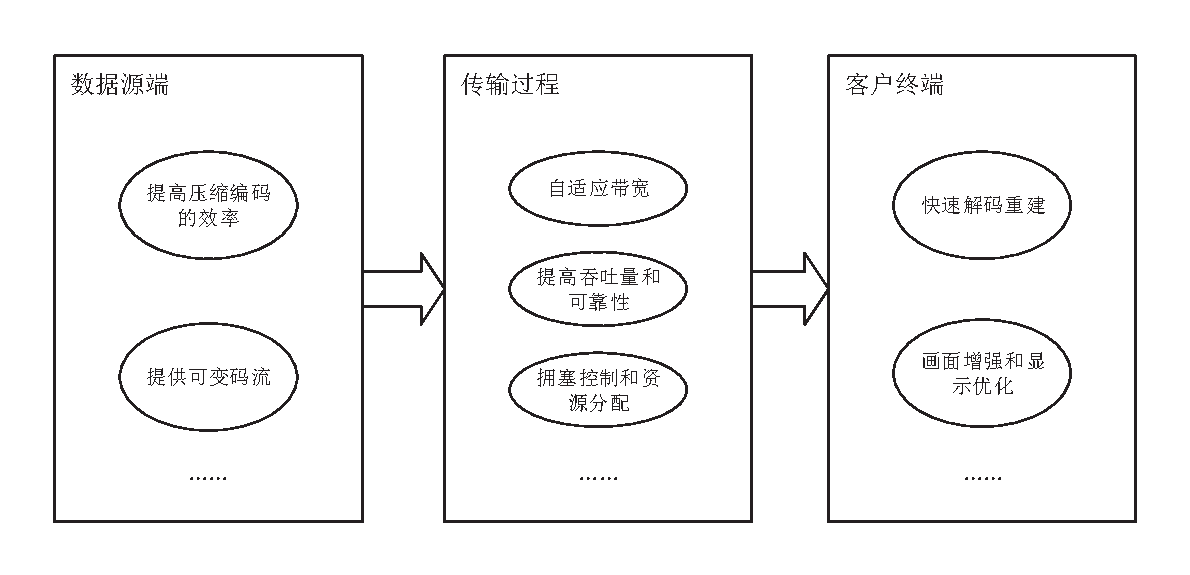
\includegraphics[width = 1.0\linewidth]{eps/research-framework}
	\caption{视频流媒体研究框架 \label{fig:research-framework}}
\end{figure}

在这一研究框架中,自适应视频流媒体主要涉及的是数据源端提供可变码率、传输过程中自动适应带宽这两个方面。虽然其他方面的研究工作,例如对编码效率的提升、对网络架构和协议的改进、在用户终端的解码优化等,也非常重要,但本文主要关注的是上述与自适性相关的两个方面(为构建高效自适应的实用视频流媒体系统所进行的客户端解码优化工作可参见本文作者已发表的其他论文)。

在视频流媒体系统中支持视频码率的可变性通常有两种选择。下面分别对其进行简单的介绍。

第一种选择是采取多码流的方法。多码流方法的原理很简单,就是预先编好不同码率的多个码流存放在服务器上,根据网络情况选取其中合适的一个进行传送。近年来兴起的HTTP动态自适应流媒体(Dynamic Adaptive Streaming over HTTP,  DASH)\supercite{Sodagar2011}就属于这类方法。如图\ref{fig:DASH}所示,DASH系统在服务器端提供不同码率的多个码流切片,客户端通过HTTP协议拉取数据,在某个时间段内可以选择性地接收这几个码流中任何一个的切片,通过在多码流之间切换来更改码率以适应带宽波动。

第二种选择是采用可伸缩视频编码\supercite{SVC-Overview}技术。作为国际视频编码标准H.264/AVC\supercite{H.264}的扩展之一,可伸缩视频编码的初衷就是在单个码流中加入伸缩性的支持,使其码率和视频质量能够根据需要改变。可伸缩视频码流中的数据被划分为基本层和增强层数据包,可以从中丢弃一部分增强层数据包而截取出一个子流,以牺牲视频质量的方式来降低码率。因此,用它来实现码率可变性正符合其设计目的。

\begin{figure}[t]
	\centering
	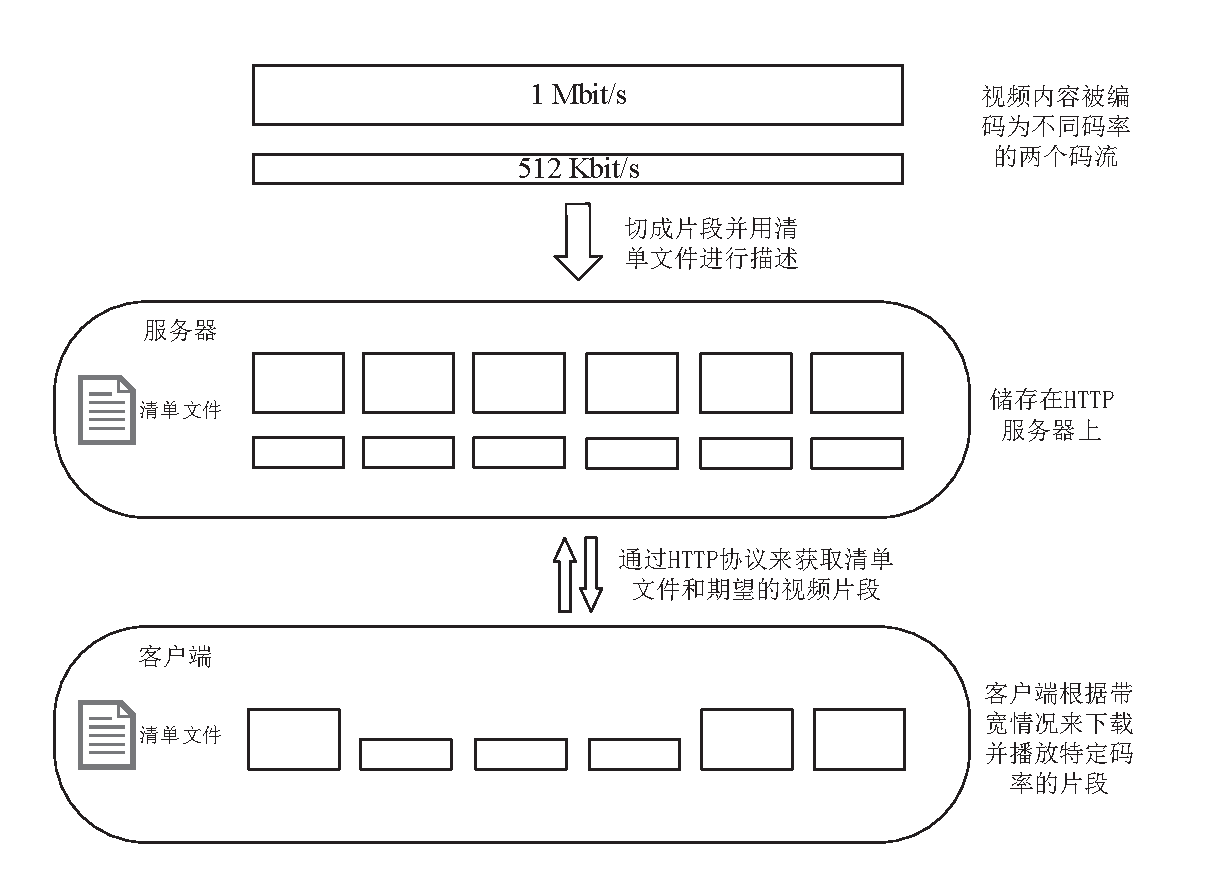
\includegraphics[width = 1.0\linewidth]{eps/DASH}
	\caption{DASH系统的工作原理示意图\label{fig:DASH}}
\end{figure}

多码流方案的优点是无需对已有的程序和系统做较大的改动,因此比较易于部署\supercite{Bouten2014}。很多商业视频网站(如YouTube、优酷等)已经用它实现了自适应功能。但是,多码流方案能提供的适应范围和粒度非常有限。例如,YouTube上的视频最多只提供144p、240p、360p、480p、720p和1080p这六个等级(参见图\ref{fig:13-1},其中右下角矩形框中显示了支持的等级),而优酷网上的视频大多只提供标清、高清、超清这三个画质(参见图\ref{fig:13}正中央的设置窗口)。此外,多个码流的编码和存储需要大量的计算资源和磁盘空间,使得时间和空间开销成倍增加。要想以合理的代价提供精细无缝的自适应性,就需要采用可伸缩视频编码的方案。可伸缩视频码流能够以非常小的数据粒度进行码率调整,而且性能分析表明可伸缩视频编码的压缩效率远高于同一内容多次编码的多码流方法\supercite{SVC-Performance}。正是因为这些优势,基于可伸缩视频编码来实现自适应视频流媒体从技术上来说是一个更好的方案,也吸引了学术界很多研究者的关注\supercite{Chuah2012, Zhu2013, Dan2013, Yang2014, Cicalo2014}。

\begin{figure}[!ht]
	\centering
	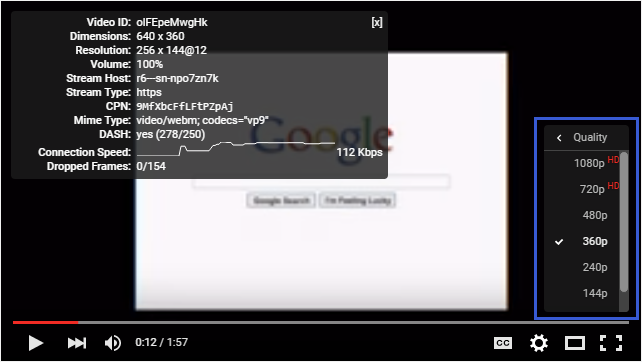
\includegraphics[width = 1.0\linewidth]{clip/13-1.png}
	\caption{YouTube视频码率自适应功能图示\label{fig:13-1}}
\end{figure}

\begin{figure}[!ht]
	\centering
	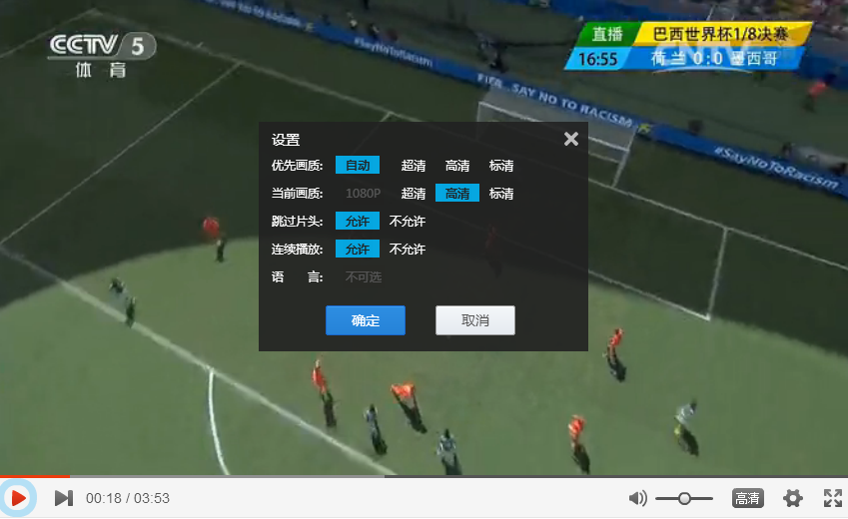
\includegraphics[width = 1.0\linewidth]{clip/13.png}
	\caption{优酷网视频码率自适应功能图示\label{fig:13}}
\end{figure}

本文的研究平台也主要是基于可伸缩视频编码的自适应流媒体系统。从图\ref{fig:research-framework}所示的研究框架中可以看出,采用可伸缩视频编码或是采用DASH之类的多码流方案,其区别只在于数据源端提供可变码率的方式不同。当可伸缩视频作为数据源时,在给定码率下选择丢弃哪些数据包,即如何最优地从整个码流中截取出一个子流用于发送是需要研究的问题之一。多码流作为数据源时则不存在这个问题。而对于在传输过程中如何自动调整码率以适应带宽的变化,却是二者共有的问题。这些问题的解决,是提高视频流媒体服务质量和用户体验的关键。

\section{本文研究内容和主要贡献}

本文结合视频流媒体所面临的挑战,对自适应视频流媒体中的关键技术进行研究,以更好地解决上面所提到的问题。首先,本文针对可伸缩视频数据源提出了新的失真模型和码流截取方案,在支持可变码率的同时提供尽可能高的视频质量;其次,本文为基于可伸缩视频编码的视频点播系统设计了新的码率自动调整策略,用控制论的方法来解决适应带宽变化的问题;最后,本文详细分析了现在非常流行的视频直播系统的传输过程,结合直播的特点提出了数据上传时的码率自适应算法。本文主要的创新性贡献可以归纳为如下三个部分:
\begin{enumerate}
\item {采用线性误差模型的可伸缩视频码流截取方案}\\
作为码率适应带宽波动的前提条件,视频流媒体中的数据源需要能够灵活调整。可伸缩视频编码技术通过将数据划分为基本层和增强层并丢弃增强层的数据包来实现即时码率变化。从完整的可伸缩码流中丢弃部分数据得到一个子流的过程称为码流截取。本文以最小化特定截取码率限制下的视频失真为目标,首先提出了一个线性误差模型来估计丢弃任意数据包组合带来的失真变化,然后利用它设计了一个贪心型算法来根据每个数据包的码率和失真影响对其赋优先级,作为截取过程中丢包的顺序。相比于参考软件,这一码流截取方案能够在同样的复杂度和码率限制下取得更高的视频质量。
\item {基于PID控制思想的点播系统码率自适应算法}\\
自适应视频流媒体中的另一个关键问题是传输过程中的码率调整策略,即在可用带宽不断变化的情况下,决定何时调整码率并确定调整到多少。本文基于经典的比例-积分-微分(Proportional-Integral-Derivative,PID)控制思想,提出了一个综合考虑带宽的历史状况、当前状态和未来趋势的码率自适应算法,既能充分利用带宽,传输较高的视频质量,又能减小带宽波动的影响,保证视频质量的平滑性。该算法集成在了苹果公司QuickTime流媒体服务器的开源版本上,并在实际应用中取得了很好的效果。
\item {基于缓冲区分析的直播系统码率自适应算法}\\
在视频直播中,由于数据是实时产生的,其传输过程与视频点播有所不同。视频数据需要先上传到服务器,然后由服务器分发到观看者进行播放。本文为这个过程中的上传阶段增加了码率自适应的特性:首先通过详细分析系统整个传输过程中各个缓冲区的关系,建立了一个多缓冲区模型;然后把上述点播系统中用到的PID方法与多缓冲区模型相结合,提出了一个有效的码率自适应算法。相比于没有自适应的上传过程,带宽的利用率得到了提升,视频播放的连续性也得到了改善。
\end{enumerate}

\section{本文的结构安排}

本文共分为六章,后续章节具体内容安排如下。

第二章概述视频流媒体领域的研究基础和相关工作。首先对视频编码和流式传输的基础知识进行简要介绍,为后文内容做准备;然后对本文所要研究的可伸缩视频码流截取、传输中的码率自适应这两个问题进行具体描述,并分析已有的相关工作。

第三章讨论采用线性误差模型的码流截取方案。首先针对可伸缩视频推导并验证线性误差模型,然后介绍采用该模型的失真估计方法和以码率失真影响为度量标准的优先级赋值算法。最后展现并分析所提出的码流截取方案的实验结果。

第四章讨论基于PID控制思想的点播系统码率自适应算法。首先对PID控制器做简单的介绍,然后将PID模型运用到视频传输中的码率调整策略,提出了一个新颖的码率自适应算法。该算法被集成在了苹果公司QuickTime流媒体服务器的开源版本中,其有效性通过对比实验得到了验证。

第五章讨论针对直播系统的码率自适应算法。首先详细分析了直播系统的传输过程,提出了一个多缓冲区模型;然后将其与PID方法相结合,选取合适的系统变量实现了上传过程的码率自适应算法,改善了带宽利用率和观看者的播放连续性。

第六章总结全文内容并对未来工作和应用前景进行展望。
	\chapter{研究基础和相关工作}

本章首先对视频编码和传输领域的一些基础知识进行概述,作为本文后续内容的铺垫;然后结合本文所涉及的研究内容,对要解决的问题进行详细描述,并对国内外研究现状和已有工作进行分析。

\section{视频的压缩编码}

原始视频信号数据量过于庞大,必须经过压缩才能有效进行存储和传输。视频信号之所以能被压缩是因为其中存在大量冗余信息,包括空间冗余、时间冗余、统计冗余等\supercite{Gao-book-2010}。以仙农信息论\supercite{Shannon-1948}和率失真理论\supercite{Berger-book-1984}为基础,通过预测(如时间预测和空间预测)\footnote{在空域或时域寻找相似信号,用与相似信号的残差来重建当前信号的一种压缩手段。}、变换(如离散余弦变换\supercite{Rao-1990}、哈达玛变换\supercite{Pratt-1969})、量化\supercite{Gray-TIT1997}、熵编码(如变长编码\supercite{Huffman-1952} 、算术编码\supercite{Rissanen-1979})等技术手段,可以去除这些冗余,以一定的失真为代价获得很高的数据压缩比。数字视频压缩编码技术经过了半个多世纪的发展,形成了一系列的国际标准。

最早的视频编码标准通常被认为是由国际电信联盟于1990年制定的H.261\supercite{H.261}。同一时期,由国际标准化组织和国际电工委联合成立的运动图像专家组(Moving Pictures Expert Group,MPEG)也开始了视频相关标准的制定工作,并于1992年推出了MPEG-1\supercite{MPEG1}。此后,以MPEG-2\supercite{MPEG2}、H.263\supercite{H.263}为代表的标准不断演进,大大推动了数字视频产业的发展。时至今日,国际电信联盟与国际标准化组织已经在标准制定方面互相合作,二者共同打造的H.264/AVC视频编码标准在蓝光光碟、高清数字视频光盘(Digital Video Disk,DVD)、数字电视广播、互联网视频共享和在线观看等各个领域都占据了主流地位,普及度极高。虽然意在取代H.264/AVC的新一代视频编码标准HEVC已经于2013年发布,但因为其编解码复杂度高且大多设备和系统尚未支持,所以还处于推广阶段。我国也制定了自己的视频编码标准AVS (Audio Video coding Standard) \supercite{AVS},但影响力远不及国际标准。考虑到上述情况,本文的研究大部分都是基于H.264/AVC及其扩展的;针对新一代视频编码标准HEVC的解码器优化也正是为了促进其推广应用。需要指出的是,随着视频编码技术的逐步成熟和定型,各种编码标准有很多共同点,因此本文的部分研究方法和结果适用于多种标准。

下面依次对H.264/AVC视频编码标准、HEVC视频编码标准、可伸缩视频编码进行介绍,作为后文研究工作的基础。

\subsection{H.264/AVC视频编码标准}

H.264/AVC的设计目标有两方面,一是显著提高编码效率,二是在网络化的趋势下满足对灵活性和可定制性的要求。为此,这一标准相对于之前的标准提出了两个新概念:视频编码层(Video Coding Layer,VCL)和网络抽象层(Network Abstract Layer,NAL)。视频编码层着重于高效地压缩和表示视频内容,而网络抽象层则用于封装视频编码层的数据并提供额外的头信息,使之适用于多样化的传输层测和存储介质(参见图\ref{fig:02}\supercite{H.264-Overview})。

\begin{figure}[h]
	\centering
	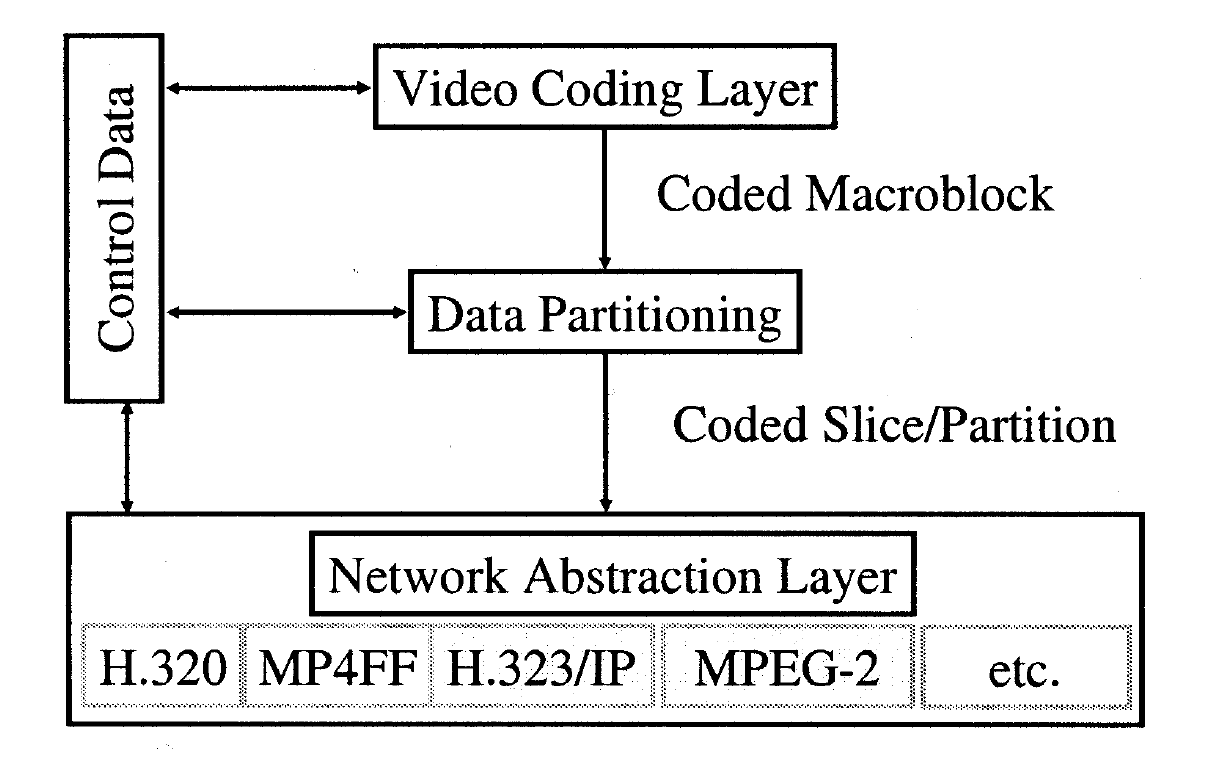
\includegraphics[width = 0.6\linewidth]{clip/02.png}
	\caption{H.264/AVC编码标准的结构\label{fig:02}}
\end{figure}

图\ref{fig:02}中,H.320是国际电信联盟制定的关于在综合数字交换网上进行视频会议的标准,H.323则是其在IP电话方面的标准,MPEG-2规定了音视频文件存储格式。可见,经过NAL层的抽象,H.264/AVC编码得到的码流可以灵活适应各种应用。下面,分别对VCL和NAL进行介绍。

VCL层的目标是高效率地表示视频内容。与其他视频编码标准一样,H.264/AVC的VCL层采用了基于块的混合视频编码框架,如图\ref{fig:03}\supercite{H.264-Overview}所示。

\begin{figure}[h]
	\centering
	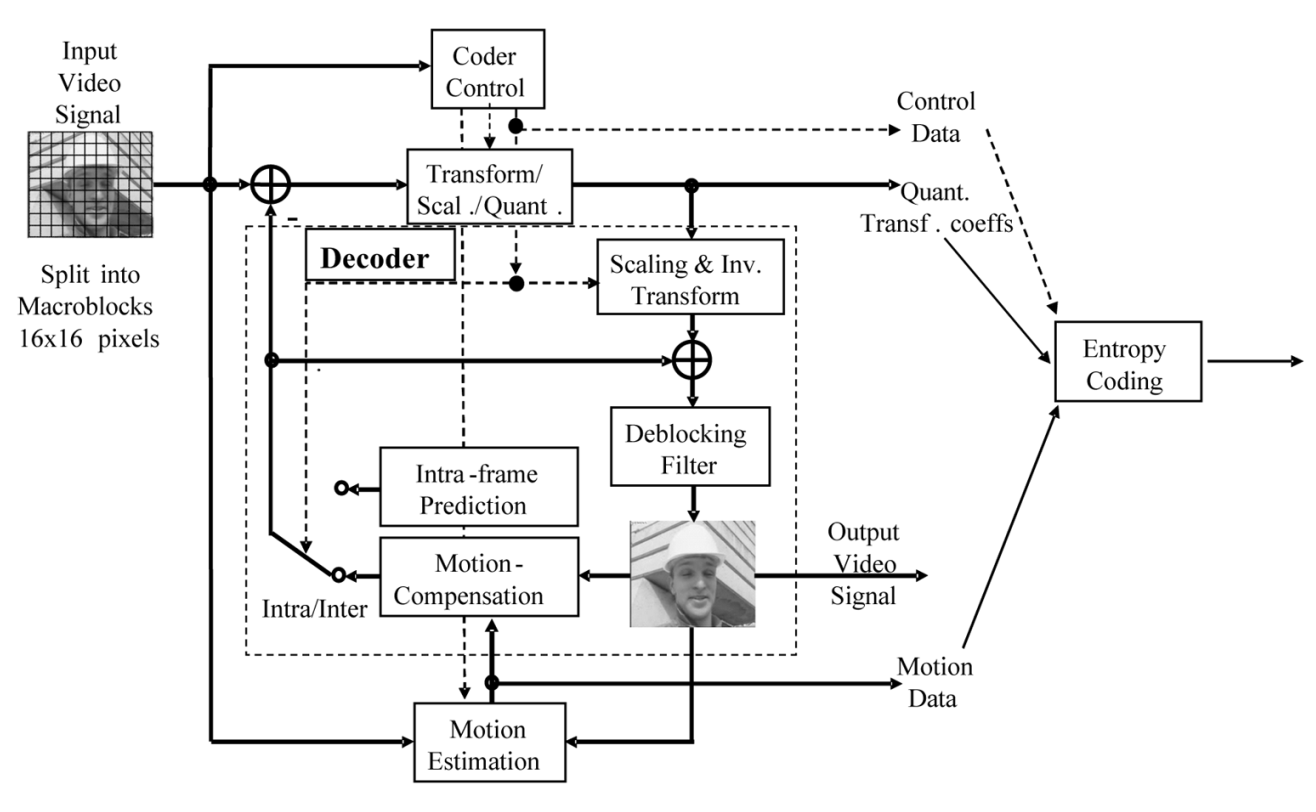
\includegraphics[width = 1.0\linewidth]{clip/03.png}
	\caption{H.264/AVC的VCL层编码框架\label{fig:03}}
\end{figure}

所谓“基于块”,是指将原始图像数据分成16x16大小的宏块(Macro Block,MB),接下来的编码过程将以宏块为基本单位。对每一个宏块,先进行时间或空间预测;预测得到的残差数据进行类似于离散余弦变换(Discrete Cosine Transform,DCT)的整数变换,然后对变换系数进行量化、重排、熵编码,最终形成比特流。

虽然这样的编码流程与之前的编码标准并无二致,但由于H.264/AVC对各个阶段进行了精心设计,并将灵活性和适应性贯穿于整个编码过程,使得其编码效率大大提高。以下仅着重分析H.264/AVC相对于之前标准的改进之处。

预测分为帧内预测和帧间预测,目的分别是去除空间和时间冗余。在H.264/AVC中,预测时可将一个宏块进一步分为小的子块进行,最小可以分成4x4的小块。标准还提供了多达9种的预测模式,从而能够更精细地利用局域特性。而对帧间预测,H.264/AVC除支持单向和双向预测之外,每个方向还允许选用多个参考帧。在运动向量的准确度上,新的标准允许精确到1/4像素,而且还允许跨越边界的值(采用外推插值技术)。

对预测残差进行变换可以进一步去除空间相关性。考虑到精细的预测模式已经很好的去除了相关性,H.264/AVC一改之前标准以宏块为单位的DCT变换,采用了更小的变换块(4x4)。而且对于相对平滑的色度值(YCbCr/YUV中的U、V),还对每个宏块中的4个4x4子块变换后的直流系数又做了一次哈达玛变换。小尺寸块的变换大大减小了计算复杂性。当然,H.264/AVC也支持将变换块扩展成16x16大小。

H.264/AVC提供了两种熵编码方法CAVLC(Context Adaptive Variable Length Coding)和CABAC(Context-based Adaptive Binary Arithmetic Coding)来去除量化后系数(以及其他一些参数)的统计冗余。它们都是上下文自适应的,前者为可变长编码,后者为二进制算术编码,后者计算较复杂但压缩率高,前者反之,可根据应用场景配置不同的算法。

以上只选取VCL的部分特性进行了简述。除了所提到的方面,H.264/AVC还包含更多可由编码器选择的配置。这样不仅能够更有针对性地去除冗余、提高编码效率,而且也增加了该标准的普适性、灵活性和可定制性。正因为如此,能够在其基础上方便地进行扩展。

VCL编码得到的比特流送去NAL层进行封装。NAL的设计目标是提供网络友好性,使得VCL数据在不同系统中的使用可以简单而高效地定制。我们后面将看到,在H.264/AVC基础上扩展得到的码流能与普通的H.264/AVC码流无缝兼容,很大程度上得益于这种网络抽象层机制。

网络抽象层的基本概念和语法结构是NAL 单元(NAL Unit,NALU)。这是一种由整数个字节组成的数据包。一个NALU以1字节的头信息起始,之后是不定长度的载荷。参见表\ref{tab:nal}。

\begin{table}[h]
\centering
\caption{H.264/AVC中的NAL单元结构}
\label{tab:nal}
\begin{tabular}{|*{11}{p{1.2cm}<{\centering}|}{p{1.2cm}<{\centering}}}
	\hline
	\multicolumn{8}{|c|}{NALU头字节} & \multicolumn{4}{c|}{NALU载荷} \\ \hline
	F & \multicolumn{2}{c|}{NRI} & \multicolumn{5}{c|}{TYPE} & \multicolumn{4}{c|}{......} \\ \hline
\end{tabular}
\end{table}

NALU字节头包含禁止位 (F,1bit) 、重要性指示位 (NRI,2bit) 、NALU类型 (TYPE,5bit) 三方面信息。其中禁止位规定为0,重要性指示位在一定意义上表示该NALU的重要程度,而NALU类型则表明该NALU中携带的是什么样的载荷。

在H.264标准中,NALU类型的0~12已被规定了用途,13~23被保留用于以后可能的标准扩展,24~31不做规定,可根据应用场景定制。按照NAL单元中载荷的不同,将其划分为两类:VCL单元和non-VCL单元。前者主要包含来自VCL的图像样本值编码数据,后者主要含有图像或序列参数集、补充增强信息(Supplemental Enhancement Information,SEI)等解码多个VCL单元所共用的一些重要数据。这种机制不仅能节省开销,也便于将重要数据通过更可靠的信道传输。对如何使用SEI来存储和传输额外的信息,后文在码流截取部分会有涉及。

\subsection{可伸缩视频编码}

可伸缩视频编码(Scalable Video Coding,SVC),简言之,就是在视频编码时生成一个包含不同层次信息的码流。从这个单一码流中,我们能够方便地丢弃一些数据,得到不同码率的多个码流,从而解码出在空间大小、帧率、画面质量等方面可伸缩的视频。虽然之前的标准也考虑了对可伸缩性的支持,但目前提到可伸缩视频编码,大多指的是H.264/AVC的可伸缩扩展。

SVC在传统编码的基础上引入了“分层编码”的概念。即对数据源一次编码得到的码流中,含有一个或多个的“层”。其中最低分辨率、最低帧率和最差图像质量的部分称为基本层,除此之外为增强层。增强层对应着更高的分辨率、帧率和图像质量。这样的码流能够提供在空间、时间、质量(或信噪比)等方面的伸缩性。当终端没有能力播放增强层或者网络无法承担高码率时,可伸缩码流的增强层部分会从比特流中移除,只有基本层数据被传送到终端解码器。
SVC编码标准得益于H.264/AVC灵活的编码逻辑结构,也继承了H.264/AVC中许多良好设计的编码工具。SVC不仅在编码效率和复杂性上与单层编码增加不多\supercite{SVC-Performance},并且完全兼容H.264/AVC。以下结合传统编码框架,在H.264/AVC的基础上,对SVC可伸缩性的实现原理进行概述。

具备时间可伸缩的码流能够根据需要动态改变视频帧率。在H.264标准中,把用于解码一帧的多个NAL单元称为一个AU(Access Unit)。SVC就是通过丢弃AU来降低帧率。时间可伸缩的实现不需要对H.264做任何增加,只需采用一种称为“层次化预测结构”的技术。

\begin{figure}[h]
	\centering
	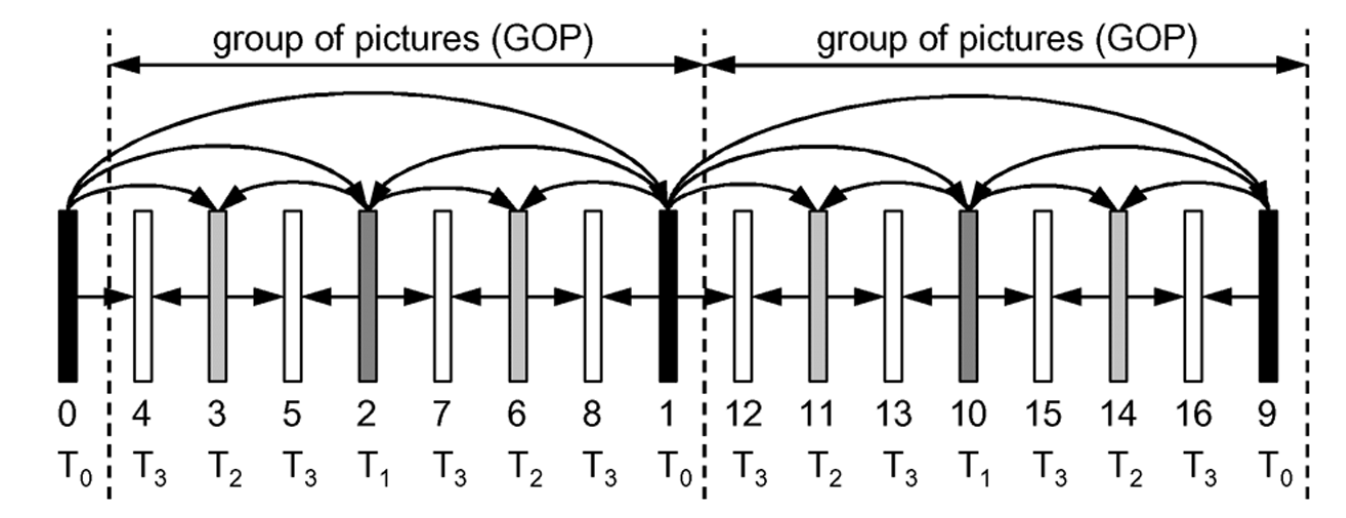
\includegraphics[width = 1.0\linewidth]{clip/04.png}
	\caption{H.264/SVC中通过层次化预测实现时间可伸缩\label{fig:04}}
\end{figure}

图\ref{fig:04}\supercite{SVC-Overview}说明了通过层次化预测来实现时间可伸缩的原理。图中一个AU下面的数字表示其编码顺序,数字下面的符号$T_i$表示其属于第$i$时间层。增强层($i>0$)的帧被编码为B帧(即参考其前后的帧进行双向预测),而且只参考较低层的帧。这样的结构下,低层的AU可以不依赖于高层,即任一较高层及其以上各层的AU可以被丢弃而不影响解码,以此实现帧率的伸缩性。需要说明的是,此例中这种“层次化B帧”的结构会带来编解码时延,且仅限于1:2伸缩比,这些不足均可通过仔细设计层次化预测结构而改善。

空间可伸缩是指视频大小的改变。空间可伸缩的实现比较复杂,需要在H.264中引入分层编码。每个分辨率都对应一个H.264编解码层,称之为“dependency layer”,由DID(Dependency ID)标记。每个层都需要不同尺寸的输入图像,这一般由最高分辨率的图像下采样得到。每层的运动补偿和帧间预测都和单层H.264编码一样,然而由于表示的是同一图像,各层之间必然有很强的相关性。SVC规定了各层之间的预测机制,称之为“层间预测”,以此来提高编码效率。

质量可伸缩顾名思义就是视频各帧的图像质量可变。这是通过丢弃一个AU中的一些质量精细化NAL单元来实现的。具体操作时,给一个AU内的每个NAL单元打上质量层标记QID(Quality ID),可以将QID高于某个值的所有NAL单元丢弃,剩下的即可组成较低质量的码流。

以上分析的主要是在VCL层实现可伸缩编码的原理,可以看到多处涉及对特定NAL单元的取舍。这就需要对H.264的NAL层进行扩展从而能够在码流中标记和传送特定的可伸缩性信息与数据。

在前面介绍H.264/AVC时曾提到,NALU头字节中的NAL类型(nal\_type)在13~23的取值留作扩展;SVC就增加了一些扩展的NAL类型。nal\_type=20的单元为新增的VCL单元,包含的是SVC中增强层的编码数据;nal\_type=14为新增的SVC前缀单元,它可能是VCL的也可能是的non-VCL的,取决于紧接着它到来的NALU。nal\_type=15的NALU用来传送SVC特有的图像参数集。对于这些新增类型的具体分析可以参见相关文档\supercite{SVC-Interface}。

普通H264解码器遇到nal\_type大于12的单元会忽略之,但能成功解码基本层,因此SVC可与之兼容。而支持SVC的解码器将对类型为14、20的NALU进行利用,实现可伸缩性。与普通H.264的NALU不同,类型为14、20的NALU并非只有1个头字节,而是扩展为4字节的头。如图\ref{fig:05}\supercite{SVC-Interface}所示。

\begin{figure}[h]
	\centering
	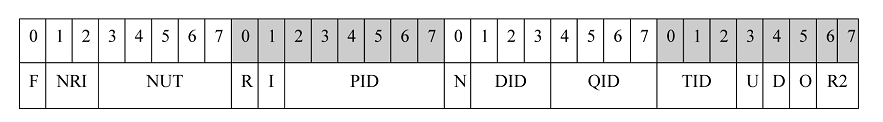
\includegraphics[width = 1.0\linewidth]{clip/05.png}
	\caption{4字节的SVC NAL单元头结构\label{fig:05}}
\end{figure}

可以看出,其中除了与普通NALU一致的第一字节,还包含了空间、时间和质量层的标志(DID、TID、QID)以及其他一些用于提供可伸缩性的信息。

根据以上分析,可在标准H.264编解码器的基础上扩展得到SVC编解码器。无论H.264还是SVC,在标准文档中都只对码流的语法语义和解码过程做了规定,换句话说:对编码的过程不做限制,只要得到符合标准的码流即可。因此编码器的程序实现可以多种多样,而解码必须与标准一致。
 
SVC标准由国际电信联盟与国际标准化组织的专家组成的联合视频小组制定。该组织在标准形成过程中还开发了一个官方的参考软件,称为JSVM(Joint Scalable Video Model)\supercite{JSVM}。该软件完整实现了SVC的编解码过程。虽然该软件未做优化很难实用,但由于其囊括了SVC标准中的几乎所有特性且清晰逻辑、配置简单,比较适合学习参考,以及作为研究性的实验平台。因此,几乎所有的学术工作都是基于JSVM参考软件,在其上实现自己的算法并与内置的算法进行对比,体现其效率的提升。本文的研究中也采用了JSVM作为比较对象。

\subsection{新一代视频编码标准HEVC}

作为新一代国际视频编码标准,HEVC的目标是相比H.264/AVC提升一倍的编码效率。HEVC仍然沿用了传统的基于块的混合编码框架(如图\ref{fig:17}\supercite{HEVC-Overview}所示),但提出了新的视频内容表示单元并引入了更加复杂的编码工具。这些新的工具目的在于提高编码效率,尤其是针对日益增多的大分辨率视频。最终发布的HEVC标准在客观和主观测试方面都已经达到了预期的目标。

\begin{figure}[h]
	\centering
	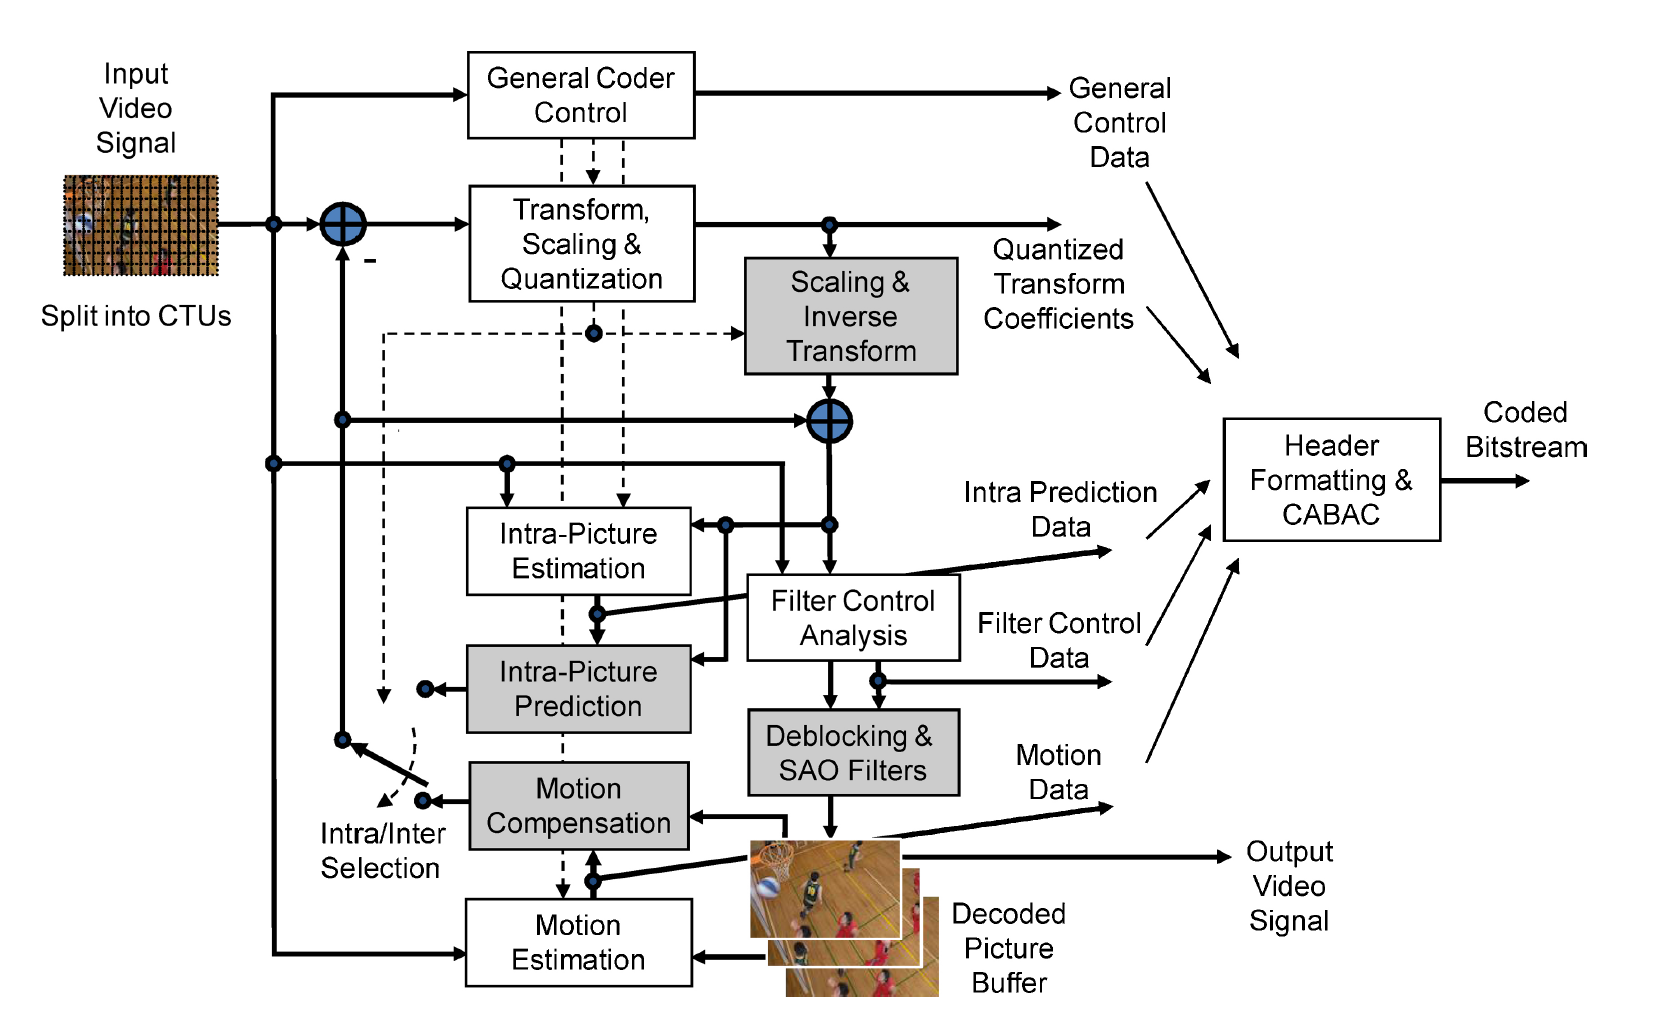
\includegraphics[width = 1.0\linewidth]{clip/17.png}
	\caption{典型的HEVC编码器结构\label{fig:17}}
\end{figure}

在H.264中,编码的基本单位是宏块(Macro Block,MB),一个宏块可以分为子宏块和块(Block)。HEVC对这种区域层次划分结构作了扩展,支持从128x128到8x8五级大小的编码单元。HEVC中的操作单元有三种,分别是编码单元(Coding Unit,CU),预测单元(Prediction Unit,PU)和变换单元(Transform Unit,TU),对应了编码的不同阶段。CU是对视频内容进行四叉树形式的划分。对一个序列在序列参数集中指定一个最大CU。最大CU可对称划分为4个子CU,最多可划分5层,可能形成128x128(最大CU)、64x64、32x32、16x16、8x8五种大小的编码单位。最终的子节点的CU进行帧内或帧间预测时被作为一个PU,所有预测相关的信息(包括预测模式、帧内预测方向、帧间预测的参考索引等)都是以PU的形式组织和传送的。根据不同的预测模式,PU内部可以进一步划分,而且这种划分可以不是对称的,这就为选择最好的预测方案提供了可能。在对残差进行变换和量化时,HEVC提出了TU的概念。一个变换单元可以与它所属的CU大小一致,也可以更精细,从而为率失真优化过程提供了更多选择。值得注意的是,TU可以包含多个预测区域,也就是说变换可以针对不同预测得到的残差进行,这对某些复杂纹理特征可以取得更好的压缩效果。

由于新的表示单元把预测、变换这些阶段独立开来,使得整个编码过程增加了更多灵活性。此外,上述单元定义使得语法元素的设计可以不受块大小的影响,采用一致的方案(在H.264中,一些语法元素的设计对于不同的块大小是不一样的),这可以简化编码规范和解码时的分析过程。

除了表示单元的变化,HEVC对H.264/AVC中的编码工具进行了扩展,或引入了一些新的技术来提高性能。以下对其中一些新特性分类作介绍。

帧间预测:运动估计的精度在原来1/4像素的基础上增加了1/12像素的精细化选项,以得到更准确的运动向量;运动校正时的插值过程改用基于DCT的插值滤波器,任意精度和任意大小范围的插值滤波参数都可以根据公式方便求得,而且非整数位置的像素值均直接由整数位置像素值计算出来;采用了更先进的运动向量预测,即预测参考可以从多个候选者中择优,不像H.264是特定的。

帧内预测:帧内预测方向扩展为任意的,不再局限于H.264的9个特定方向,以适应大分辨率视频的特点;对每一个PU,预测得到的值可以进行平滑处理从而更利于接下来的残差变换;新标准的预测机制还考虑了不同颜色分量之间的相关性、像素模板匹配、预测结果与原像素值的加权组合等多种因素,共同提高帧内预测的效果。

空间变换:仍然采用类DCT的整数变换,但考虑到新的优化算法的出现以及对编码大分辨率视频的需求,变换块的大小增加至16x16、32x32甚至64x64;而且在整数变换之后,还可以增加一个旋转变换来更好压缩某些强对角分量的残差。

环内滤波:为消除块效应、降低重建图像和原图的误差,需要对重建图像做去块滤。新标准的去块滤波在H.264的基础上增加了随CU的适应性,即可对不同单元选择打开或关闭这一滤波过程。此外,为进一步消除误差,还引入了其他纠正措施作为后处理过程。

熵编码:主要还是H.264中的CABAC编码,但一方面增加了对不同语法元素的适应性,另一方面对编码前的系数扫描过程也提供了多种模式(Zig-Zag,横向,竖向)供择优选取。

采样自适应偏移(Sample Adaptive Offset,SAO):增加到了环内去块滤波之后,旨在进一步改善重建图像质量。

从最早的H.261到现在的H.264/AVC、SVC,再到最新的HEVC,一系列视频编码标准的制定和推广过程不仅促进了产业发展,还在以下两个方面催生了大量的学术研究成果。一是对信源编码理论及应用的研究,包括对图像视频中不同信源的概率分布建模\supercite{Birney-TIP1995, Lam-TIP2000, Sharifi-TCSVT1995, Kamaci-TCSVT2005},对特定信源分布下率失真函数和量化器性能的分析\supercite{He-TCSVT2001, Gary-TIT1996, Gary-VCIP2005},基于率失真分析和估计来改进编码中的率失真优化和码率控制过程\supercite{Gary-SPM1998, Lin-TCSVT1998, Sun-TCSVT2006, Lee-TCSVT2014},等等;这些研究旨在不断提高压缩效率和编码器性能,是视频产业链上后续相关环节的基础。二是视频编码与网络传输相结合的研究\supercite{Sun-book-2001},包括在Internet上传输视频\supercite{Wu-TCSVT2001, Conklin-TCSVT2001},采用可伸缩视频编码以应对网络异构和拥塞导致的带宽波动\supercite{Wu-IEEE2001, Ohm-IEEE2005},等等。这方面的研究则直接推动了视频流媒体应用不断改善和蓬勃发展。本文的工作主要偏向于上述第二方面。下面对视频流媒体相关知识进行介绍。

\section{视频文件的流式传输}

流媒体系统之所以能够在不必下载完整音视频文件的情况下进行播放,主要是因为采用了流式传输。流式传输的对象是存放在服务器上的流式文件。生成流式文件是流媒体系统的起点。流式文件经过了特殊编码,使其适合在网络上边下载边播放。对于编码压缩好的视频文件,需要将数据分成适当大小的分组并考虑差错恢复功能,此外一般还要加入特定的时间戳和索引(hint或index)信息,用于提供如快进、后退和随机访问等控制功能。上述过程称为媒体文件的流化。流化得到的流式文件存放在服务器上等待传输。

流式传输是流媒体系统的关键。通常流式传输可以分为两种:顺序流式传输和实时流式传输。顺序流式传输虽然也能边下边播,但用户只能观看已下载的部分,不能跳到未下载的前面部分。这种流式传输方式通过HTTP即可实现,不需其他特殊协议,但其功能和特性也不够灵活。与之相对应的是实时流式传输。这种方式允许用户对媒体流的发送进行更多的控制,可随机访问前后内容。相应地,这种传输方式也需要特定的服务器和特殊的协议。图\ref{fig:10}给出了典型的流媒体视频点播系统的基本框架。

\begin{figure}[h]
	\centering
	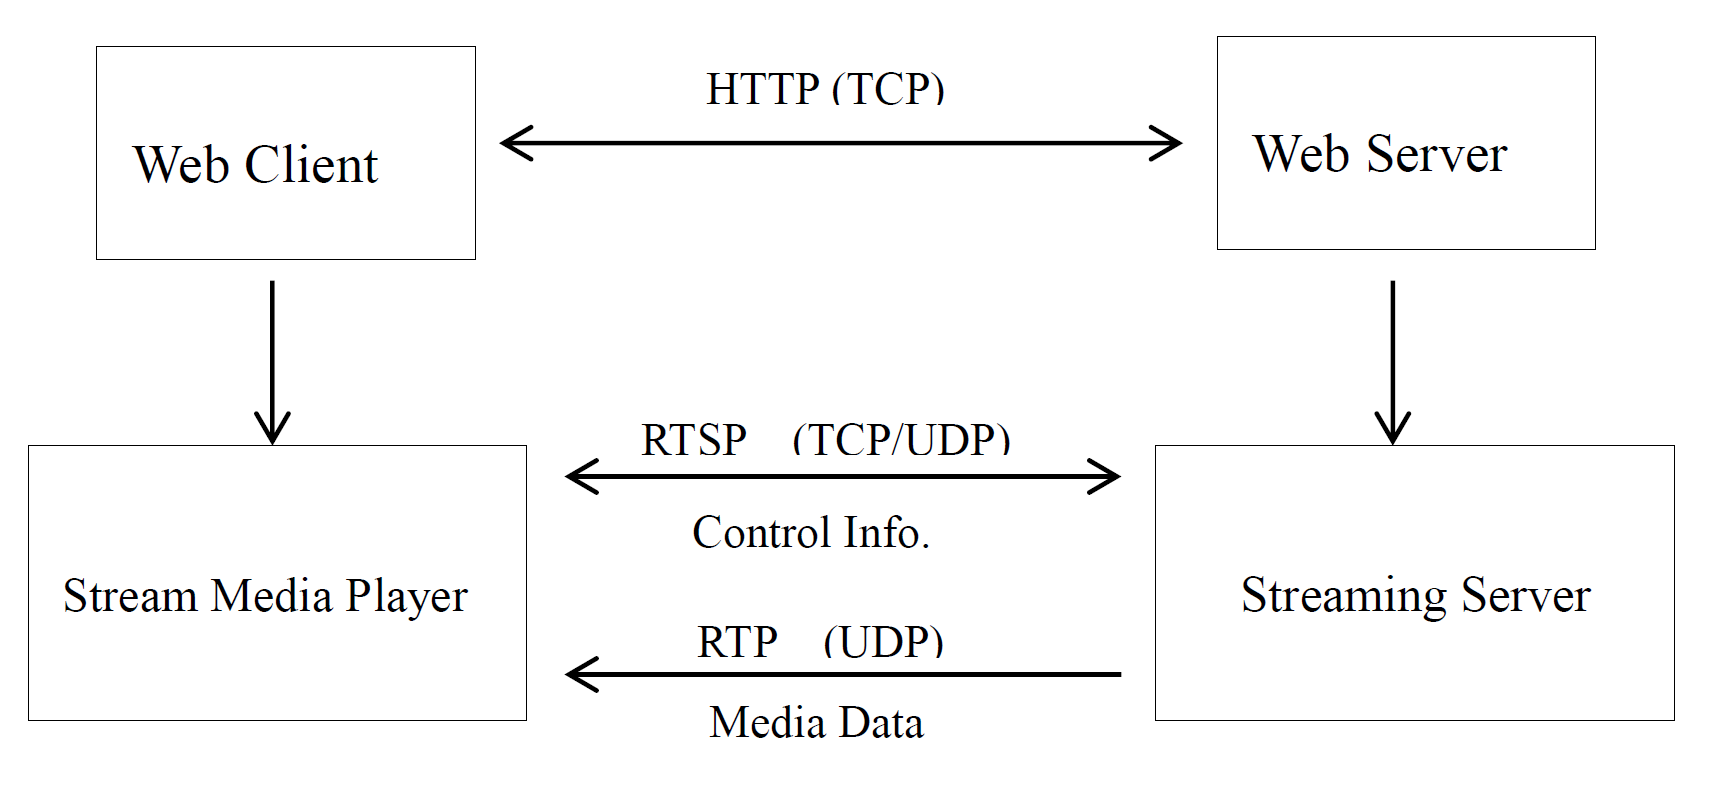
\includegraphics[width = 1.0\linewidth]{clip/10.png}
	\caption{典型的流媒体应用框架\label{fig:10}}
\end{figure}

图\ref{fig:10}可见,通过流式传输播放在线视频的一般过程如下:
\begin{enumerate}
\item 用户根据观看意愿检索和选择视频;在Web浏览器与Web服务器之间通过HTTP/TCP进行通信。
\item Web浏览器利用从服务器得到的参数对客户端的流媒体播放起进行初始化;这些参数包括流媒体服务器地址、目录和媒体文件信息等。
\item 播放器与流服务器之间运行实时流控制协议(Real-Time Streaming Protocol,RTSP),进行A/V 数据传输的控制,如准备、开始、暂停、后退等。
\item 流服务器使用实时传输协议(Real-time Transport Protocol,RTP)将媒体数据传送给客户端,数据抵达时即可解码播放。
\end{enumerate}

流媒体是面向网络的应用,既需要终端软件,也需要传输和控制协议。本节剩余部分中,首先介绍流媒体传输用到的几个典型协议,然后介绍代表性的流媒体服务器。

\subsection{典型的传输协议}
\label{subsec:protocols}

实时流协议RTSP是一种应用层协议,其目的是为了在IP网络中有效传输流媒体数据。RTSP本身并不发送媒体数据内容,它主要起到建立流和控制流的作用。RTSP类似于HTTP,在客户端和服务器之间发送请求和回应。一般会有以下交互:
\begin{itemize}
\item OPTIONS: 客户端询问服务器有哪些操作,服务器进行回应,列出可用的方法。
\item DISCRIBE:客户端向服务器请求描述信息,服务器以会话描述协议(Session Describe Protocol,SDP)的形式返回该信息,包括音视频的编码类型、参数,控制通道等等。
\item SETUP:客户端在得到媒体信息后建立流;对音频、视频需要分别建立。
\item PLAY(类似的有PAUSE、SCALE等):开始播放媒体(或进行控制)。服务器在收到PLAY后会开始以RTP协议发送媒体数据包。
\item TEARDOWN:客户端请求关闭流。
\end{itemize}

可见,RTSP只在播放流媒体之前和结束时发挥作用。实际传输数据采用的是实时传输协议RTP。

实时传输协议负责传输媒体数据。它是单向的,将流媒体内容以包的形式从服务器发送至客户端。RTP包由头信息和载荷组成\supercite{RTP}。包头中提供了版本号、有效载荷类型、时间戳、序列号等信息,并且允许扩展。包的载荷则是实际的音视频编码数据。接收端解码时必须知道RTP载荷中数据的编码方式,包头中的有效载荷类型即标识了这一信息。有效载荷类型域共7bit,可表示多达128种载荷。除了标准中指定的类型外,还可以进行扩展。

可以用指定有效载荷类型的RTP包来表示所传送数据的编码方式为H.264。此时,RTP载荷(payload)将呈现为H.264定制的结构\supercite{RTP-H.264}。H.264的一个NAL单元大小不定,有时会超过一个RTP包的容量(受限于RTP下层协议的包大小,如UDP);有时又较小,可将多个NAL单元封装在一个RTP包中。为此,针对H.264的RTP载荷将第一个字节作为头字节来标记上述的分拆和组合。事实上,H.264的RTP载荷的第一字节采用的结构与NAL单元的头字节相同,并且各个比特的意义也一致。其中后5bit表示该RTP包中的NAL单元的类型,若为0~23则表示H.264标准的一个完整NAL单元,大于24的被用来表示拆分或组合NAL单元。

RTP为包括H.264在内的不同标准流媒体数据提供了有效的传输支持。但它却是不可靠的,它本身没有任何错误检测或拥塞控制机制,因此无法提供QoS(服务质量)保证。RTP底层可以使用UDP也可以使用TCP,但大多采用的是UDP。而且RTP一般与下面介绍的实时传输控制协议(Real-time Transport Control Protocol,RTCP)配合使用。

实时传输控制协议RTCP被设计用来监测流媒体传输质量并在RTP会话参与者之间传递信息。RTCP包可携带不同类型的信息,其中最典型的是接收者报告。这种RTCP包由接收者向服务器发送,报告其收到的RTP包数目、丢包数、包的抖动、延时情况等。这相当于提供一种反馈信息,发送端应用程序可以利用这些信息做出调整,如改变发送速率等。一般流媒体软件都会利用RTCP来控制和保证传输质量。

\subsection{流媒体服务器}

实用的流媒体系统离不开服务器端软件和客户端播放软件。客户端软件主要是支持播放流媒体,为此除了普通媒体播放功能,还需要实现RTSP、RTP等网络协议,但总体来说比较简单。下面着重对流媒体服务器端程序进行介绍。

在流媒体服务器上运行的程序负责响应连接请求,从存储系统中取出音视频数据并以流式传输的方式发送给客户端。完整的流媒体服务器平台需提供会话服务、内容服务、流服务、媒体数据存储管理等(参见图\ref{fig:11})。目前市场上应用较多的流媒体技术和平台主要有三种:RealNetworks公司的RealSystem,微软公司的Windows Media,以及苹果公司的QuickTime。它们分别有各自的流媒体服务器和播放器。前两家的产品都只有闭源的商业版,而苹果公司的流媒体服务器除了商业版本外,还同时提供开源的版本,称为达尔文流媒体服务器(Darwin Streaming Server,DSS)\footnote{http://dss.macosforge.org/}。该服务器经常被用来做相关的研究测试\supercite{Huang2004},本文在视频点播方面的码率自适应研究就是基于它进行的。

\begin{figure}[h]
	\centering
	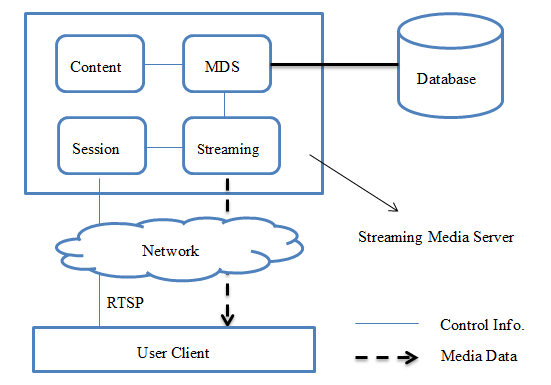
\includegraphics[width = 0.9\linewidth]{clip/11.png}
	\caption{流媒体服务器的组件及其与外界的交互\label{fig:11}}
\end{figure}

原本的达尔文流媒体服务器是不支持SVC的,为了本文的研究和实际的应用,可以在其源代码上修改使其增加对SVC的支持。达尔文流媒体服务器包含多个工程,其中负责流发数据的主要集中在StreamingServer工程中。在这里,由RTSP协议与客户端建立连接会话,并在客户端的SETUP命令下建立多个音频和视频的流,然后由RTP协议向客户端发送数据。每个会话对应一个RTPSession类,每个流对应一个RTPStream类,RTPStream类的Write函数起到实际的发送数据功能。实现对SVC的支持主要是在此类中改变向流中写数据的逻辑。当然,前提是数据的来源必须是SVC的。

达尔文服务器处理的媒体数据来源于特定的MP4文件。正如前文提到的,与本地播放的普通MP4文件不同,用于流式传输的MP4必须经过hint处理(即流化)。流化后的MP4文件不仅包括对应音、视频的audio track和video track,还包括一个hint track,其中信息用于流式传输。SVC的MP4文件区别于非SVC的地方就是在hint track中有SVC伸缩层的数目信息,因此要采用特定的SVCCreator工具来打hint。SVCCreator在打hint时会将SVC视频流所支持的空间、时间、质量层数目写入hint track。这样流化得到的MP4文件就是支持SVC的,可送给达尔文服务器。达尔文服务器在接受到客户端的DESCRIBE命令(以RTSP发送)后,会解析MP4文件中的相应媒体信息,以SDP的形式发给客户端。SDP中包含了音视频的参数,其中可以任意添加参数项。我们在描述视频的参数中加入svclayercount这一项,把从hint track读到的空间、时间、质量层数目告诉客户端。这就使得客户端可以主动设置想要接收的层。这只是提供一种支持,客户端也可以完全不主动设置,服务器会根据网络状况自动调整发送的增强层数据。具体如何调整,就是本文所要研究的码率自适应问题。

\section{可伸缩视频码流截取}

\subsection{问题描述}

可伸缩视频码流截取使视频码率可以动态调整,是基于可伸缩视频编码进行自适应流媒体传输的基础。所谓码流截取,是指从一个完整的码流中抽取所有数据包的一个子集,得到一个更低码率的子流的过程。图\ref{fig:Bitstream-Extraction}展示了一个可伸缩视频码流的结构,以及从中截取子流的一种可能的方式。
可以看到,该码流中的数据包被分为了不同的层。时间层(T0~T3)反映了各帧之间的参考或依赖关系。图形上方的箭头从被参考帧指向参考它(也就是依赖于它)的帧。质量层(Q0~Q2)反映了一帧之内的视频质量伸缩性。处于高层(也就是Q1和Q2层)的数据包可以被部分丢弃从而实现码流截取。图中的虚线表示了一个截取的例子。虚线上方的数据包全部被丢弃,只有虚线下方的数据包保留在截取出来的子流中。

\begin{figure}[h]
\centering
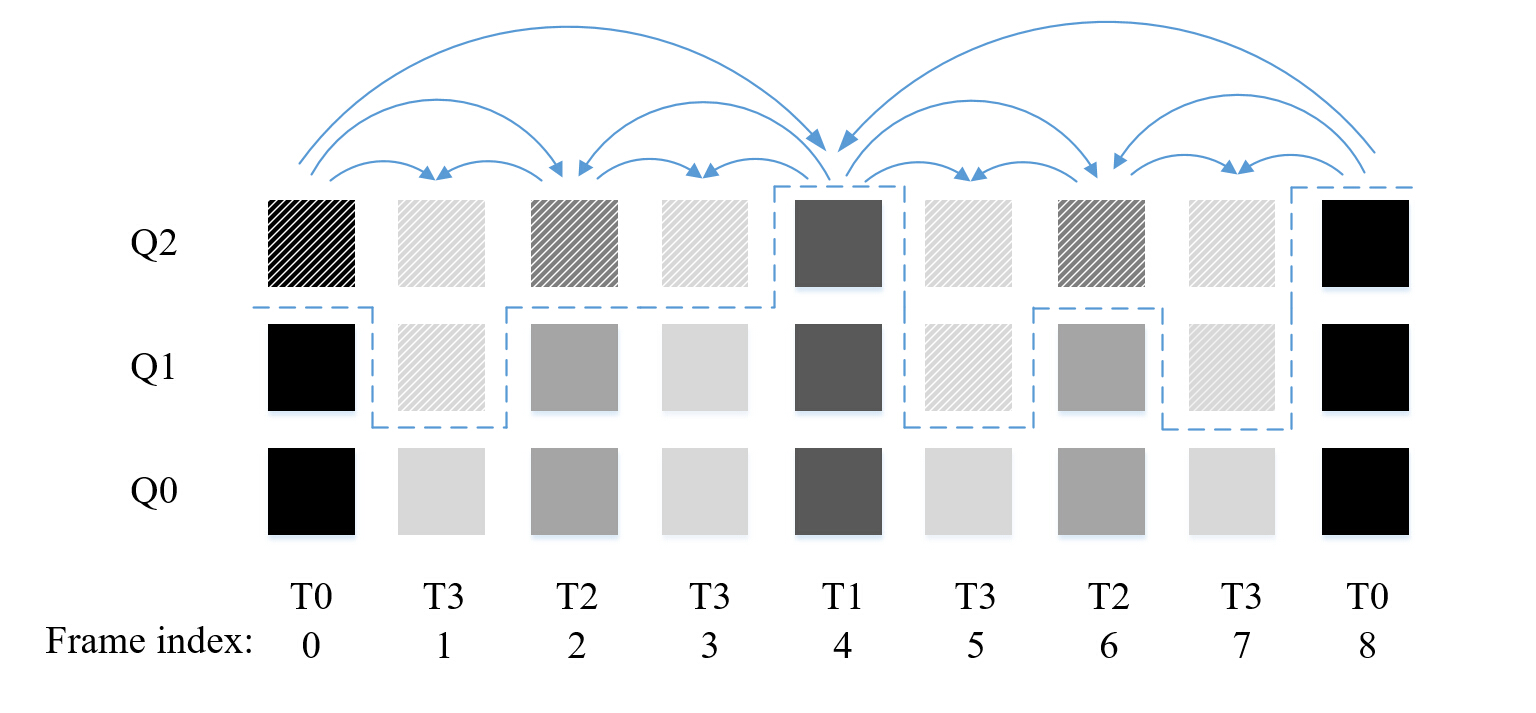
\includegraphics[width = 0.9\linewidth]{./figures/Bitstream-Extraction.jpg}
\caption{可伸缩视频码流截取示意图\label{fig:Bitstream-Extraction}}
\end{figure}

容易发现,可伸缩视频码流截取从本质上来看其实是一个组合优化问题。在所有的数据包中,我们希望在给定的码率限制下,选出一个最优的数据包组合,使得它们构成的子流具有最大的视频质量。如果用$R_T$表示码率限制,$\theta$表示某种截取方案,那么码流截取问题可以用下面的式子表示:
\begin{equation}
{\theta}^* = \mathrm{arg} \min \limits_{\theta \in \Theta} D(\theta), \quad  \mathrm{s.t. } \quad R(\theta) \le R_T.
\end{equation}

其中$D(\theta)$和$R(\theta)$分别表示这种截取方案下对于的失真和码率。

更准确地说,这个问题与大家所熟知的“0-1背包问题”\footnote{http://en.wikipedia.org/wiki/Knapsack\_problem}在形式上是一致的。每个数据包可以看作是一个具有特定重量和价值的物品。这里的重量就是数据包的大小,价值就是它对重建视频质量的贡献。码流截取的过程就是决定每个数据包是否包含在最终的子流里。用“0-1背包问题”中的术语来说,就是选择将哪些物品放入背包中。

对于典型的“0-1背包问题”而言,其最优解可以用动态规划的方法得到。然而对于码流截取问题来说,这个方法是不可行的。主要原因在于数据包之间的依赖关系。首先,截取的数据包子集不能任意挑选,因为如果一个包被包含进了子流中,那么这个包所依赖的数据包也必须被包含进去,否则将无法正确解码。例如,在图\ref{fig:Bitstream-Extraction}中,我们不能只选择一帧中的Q2层数据包而丢弃同一帧的Q1层。其次,不同于“0-1背包问题”中定义良好的物品价值,码流截取问题中一个数据包对最终视频质量的贡献并不是明显且确定的。这是因为,数据包所在的帧在解码中是互相参考的,它们对视频质量的影响会互相干扰,对于不同的截取方案,每个数据包的实际贡献可能有所不同。事实上,除非实际进行一遍截取、解码、计算的操作,我们甚至无法准确地得到所截取出的子流的真实视频质量。这就使得可伸缩视频码流截取问题成为了一个复杂得多的问题。

\subsection{相关工作简介}

就我们所知,学术界没有人提出过一种确定能找到码流截取最优解的方法。当然可以用暴力穷举的方法来解决这个问题,但其复杂度显然是无法接受的。相关的工作都是尽可能用较低的计算量获得较好的次优解。下面对可伸缩视频码流截取的相关工作做简要的介绍。

\begin{figure}[h]
	\centering
	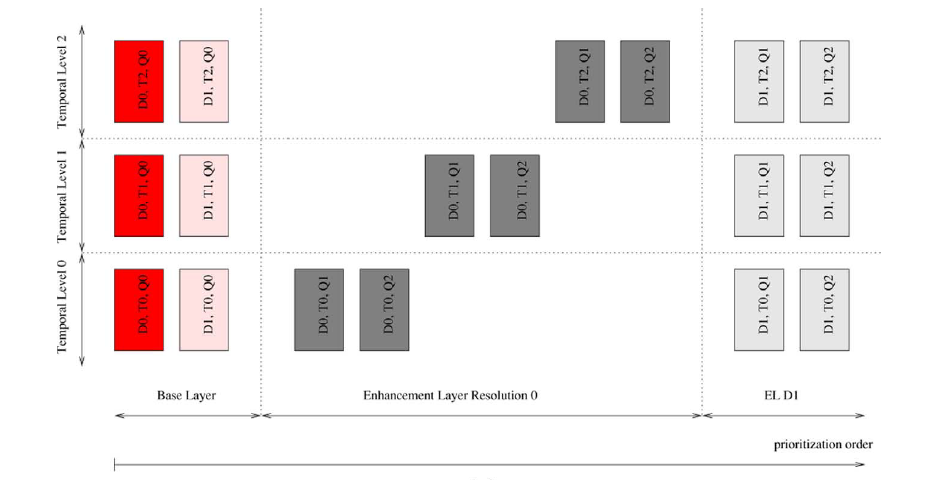
\includegraphics[width = 1.0\linewidth]{clip/06.png}
	\caption{JSVM基本截取器的算法图示\label{fig:06}}
\end{figure}

最初的参考软件JSVM提供了一个非常简单的基本截取器。该截取器并没有考虑任何优化,只是实现了一个从完整码流中丢弃一些层的包来使码率低于给定值的程序。如图\ref{fig:06}所示,该程序按照SVC中的层的概念将所有NAL数据包分成了几组,在截取丢包的时候,高层的包先丢,如果整个高层都丢弃之后仍然不能满足码率要求,再考虑丢低层的数据包。这种方法符合直观理解,因为一般来说低层的数据作为被参考对象,影响的范围更广,重要性更大一些,所以应该优先保留;反之,高层的数据可以先丢。但编码过程中形成的数据包之间的关系并没有这么简单,有可能某个高层的包比某个低层的包更重要,基本截取器并没有考虑这一点。因此,基本截取器的效果离最优还有很大的差距。此外,对于同一个层的数据包,基本截取是按某个固定的顺序依次丢弃,也并没有对这些同一层数据包的重要性做区分。这也是基本截取器效率低下的另一个原因。接下来介绍对基本截取器的改进工作。

Amonou等人\supercite{Amonou2007}提出了一个基于“Quality Layers”的码流截取方案。这一方案被SVC参考软件JSVM所采用,而且取得了比JSVM中的基本截取器更好的性能。在Amonou等人的方案中计算了一个“Quality Layers”(简称QL)值,它反映了一个数据包(NALU)的码率失真影响,据此进行截取能得到率失真优化过的结果。对于计算出来的QL值,可以用两种方法将其存储在码流中:

\begin{itemize}
\item 占用NALU头信息中的priority\_id字段来存储这个NALU的QL值。这个字段有6比特,只能存储64个不同值;
\item 用专门的补充增强信息(SEI)数据包来存储所有NALU的QL值。
\end{itemize}

在计算QL值的时候,对数据包失真影响的估计是一个计算量非常大的过程,而且估计的准确性也有提高的空间。因此,后续工作提出的失真模型一方面是降低复杂度,另一方面是进一步提高准确度。Sun等人\supercite{Sun2009}和Maani等人\supercite{Maani2009}所构造的模型都是基于帧间的误差漂移来计算失真。Sun等人的模型在性能方面几乎与JSVM相当,但计算复杂度却大大减少。而Maani等人的模型取得了比JSVM更高的估计准确度(由图\ref{fig:15}\supercite{Maani2009}可见,其估计的失真与实际失真基本相同),但是由于其是基于训练的,为了得到更鲁棒的模型参数,需要更大的计算量。

\begin{figure}[h]
	\centering
	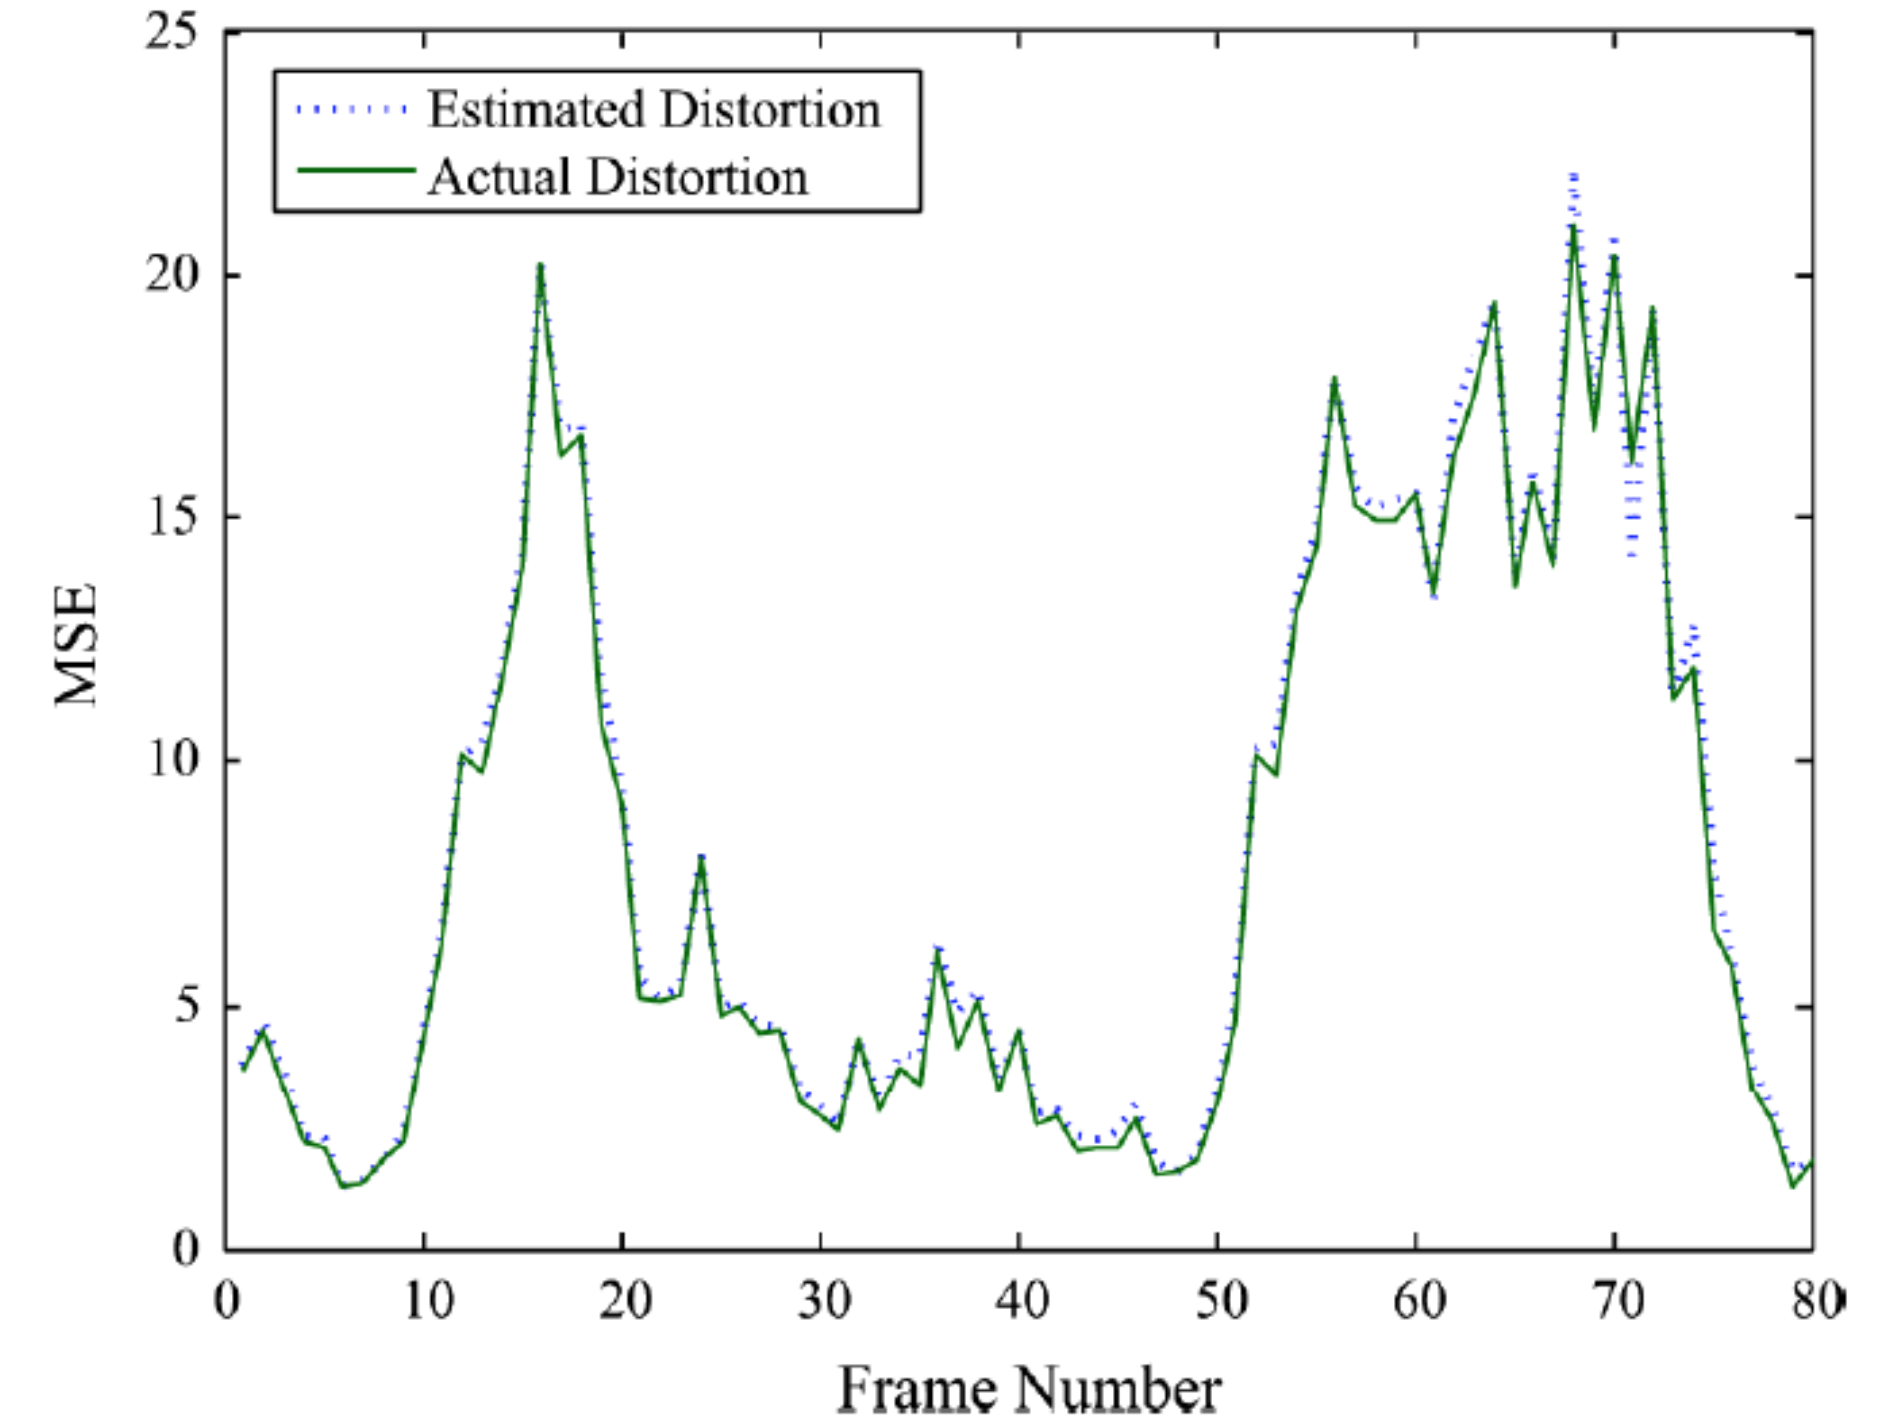
\includegraphics[width = 0.8\linewidth]{clip/16.png}
	\caption{基于训练的模型所取得的失真估计准确度图示\label{fig:16}}
\end{figure}

此外,Ramanathan等人\supercite{Ramanathan2012}提出了一个“Quality Metadata”的概念来用于码流截取,这与上面所说的“Quality Layers”是同样的思想,只是计算方法有所差别;Yang等人\supercite{Yang2013}提出了一个基于模拟退火的方法来解决码流截取问题,他们简单地用丢弃较低增强层数据带来的失真来估计丢弃较高增强层数据带来的失真。因为码流截取从另一个角度看是丢弃数据包的过程,丢弃的先后顺序可以认为是这些数据包的优先级。于是一些研究者从赋优先级的角度来提出相应的算法。例如,Lim等人\supercite{Lim2006}把可伸缩视频码流视为树形结构并据此来为每个数据包赋予优先级,而Zhu等人\supercite{Zhu2011}则采用拉格朗日乘子方法计算优先级值。在这些已有的工作中,失真估计的准确性都显著地影响最终结果。因此,提出简单有效的误差或失真模型对于码流截取的研究至关重要。本文的研究工作正是在此处着力并取得了创新性成果。


\section{传输中的码率自适应}

\subsection{问题描述}

在数据源具备码率可变的前提条件之后,实际传输时就可以根据带宽来调整发送的速率。改变码率去适应带宽的变化,这就是所谓的码率自适应问题。对于一个码率自适应算法,有三个最基本的目标。这三个目标可以用来衡量自适应算法的效果,也是设计算法时需要考虑的方面。下面分别进行描述。

对于一个流媒体系统,最首要的目标应该是保证视频播放能够连续不断。一旦视频开始播放,每个数据包都有了自己的显示时间。这个时间也决定了传输的截止时间。如果这个数据包没有在截止时间前达到客户端,那么客户端播放器就会因缺少数据而暂停。这就是用户所遇到的卡顿现象,应该努力避免。避免卡顿一般要依赖于传输中的缓冲机制。如果检测到带宽下降、当前码率确实过高,应及时下调质量,以防止数据不能按时传送而导致播放卡顿。

其次是要保持视频质量的平滑性。网络条件变化可能比较剧烈,但视频质量应该尽可能维持在一个比较稳定的水平。因为频繁的质量调整会给用户带来反感。举例来说,当用户适应了较低的质量后,突然调高质量并在短时间内又调低,给用户的体验还不如不调整。因此,在保证播放连续的前提下,应尽可能减少质量调整次数,充分利用缓冲区的作用,避免因为临时或短暂的带宽变化就调整质量。

最后,还要提供给用户尽可能好的视频质量。假设我们一直发送较低码率的视频流,那么既能保证播放的连续性又不存在平滑性的问题,上述两个目标可以轻而易举达到。但是这样的话用户看到的视频质量将一直处于较低的水平,显然不是令人满意的选择,所以不可取。码率自适应算法应该能够充分利用可用带宽,在带宽足够的情况下提高发送质量,给用户最好的观看体验。

综上所述,在视频流媒体的码率自适应研究中,保证播放流畅是最基本的要求,同时视频的高质量和平滑性也是所追求的指标。

\subsection{相关工作简介}

码率自适应的研究主要集中于如何选择和调度视频数据包。Gao等人\supercite{Gao2006}提出的调度策略首先确保重要性较高的数据优先发送,而对于重要性相同的数据包,播放时间最早的首先发送。Schier等人的工作\supercite{Schierl2010}也与此类似,把视频数据放在具有不同优先级的缓冲区中(参见图\ref{fig:15}\supercite{Schierl2010}),通过调整优先级来确保数据及时发送。在达尔文流媒体服务器中内置有一个被称为包延迟反馈的调度算法。当一个包要发送时,服务器会检测它的延时(即这个数据包应播放的时间和当前时间的差),并根据这个延时来判断当前发送顺畅还是阻塞,以此来推测带宽情况,并相应调整发送码率和质量。具体判断方法是将这个延时作为反馈,与预先设定的阈值进行比较。例如,预先决定当前带宽下发送某个数据包之后T时间内应该播放,那么理想延时应该保持为T。如果发现延时小于T了,说明发送受阻,可能是带宽减小了;反之,如果T变大了,说明发送顺畅,可以考虑增加质量。这种算法能够在一定程度上检测带宽的变化并作相应调整。但是它的调整策略是保守的,在它检测到延时变小时,很可能客户端已经因为缺少数据而停止了。而且该算法对带宽的变化趋势也不能提前预测,很可能导致质量波动,这也是需要改善的一个问题。

\begin{figure}[t]
	\centering
	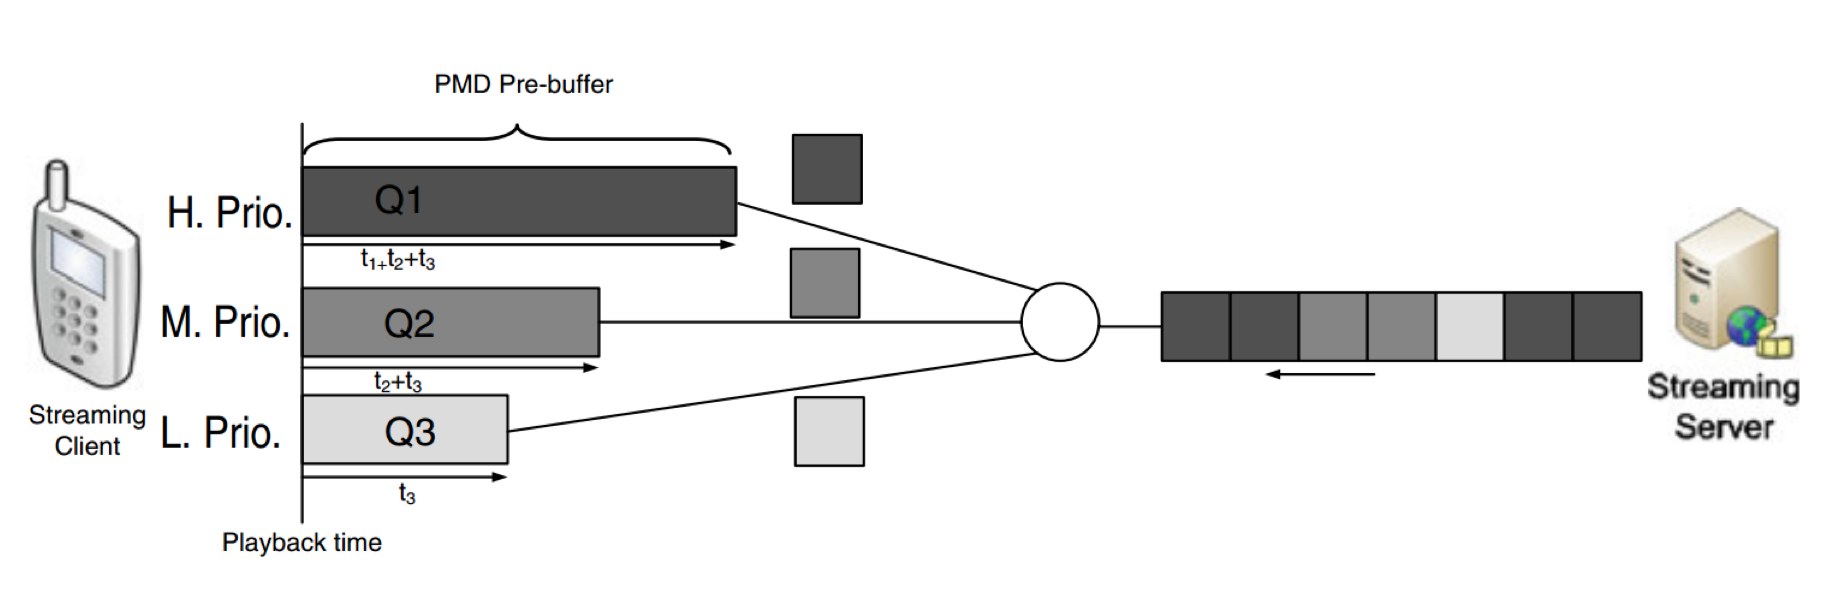
\includegraphics[width = 1.0\linewidth]{clip/15.png}
	\caption{基于不同优先级缓冲区的码率自适应算法\label{fig:15}}
\end{figure}

上面的工作都是针对可伸缩视频流媒体系统或是RTSP传输协议进行的。对于HTTP动态自适应流媒体(DASH),国内外也已经有了不少研究。例如,Akhshabi等人\supercite{Akhshabi2012}分析了来自商业公司和开源社区的多个DASH客户端播放器的自适应行为,比较了他们之间性能的优缺点。张辉帅等人\supercite{Zhang2013}提出了一种基于拉模式的码率自适应算法,利用滑动窗口分析最近若干分片的下载时间,基于此来选择最合适的码流。Huang等人\supercite{Huang2015}结合了缓冲区的状态和对带宽容量的估计这两个判据来做如何调整码率的决策。Juluri\supercite{Juluri2015}等人考虑到每个分片数据量大小不同可能导致下载时间的差异,因此提出了一种提前查看分片信息的码率自适应算法。

这些已有的研究工作在一定程度上提高了传输效果,但大都是针对点播模式,没有考虑到直播模式下的特殊问题。目前实时性直播的应用越来越广,从某种程度上来说是一个更重要的模式。直播由于其数据是实时产生的,无法提前加载,因此与点播有所不同,需要进行针对性的研究,设计新的码率自适应算法。本文的工作不仅适用于点播系统,也能很容易扩展应用到直播系统中。

\section{视频解码优化}

视频解码器优化的工作总是紧密结合视频编码标准而进行。本文主要关注最新的国际视频编码标准HEVC的相关工作。自HEVC推出以来,不少论文都针对其解码器实现和优化进行了研究。大部分已公开的研究工作都是在标准化组织所提供的参考软件HM\supercite{HM}的基础上进行的。在HM之外,我们所能查到的在正式发表文献中提出的独立解码器实现只有少数几个\supercite{Bossen-TCSVT2012,JCTVC-G988,JCTVC-H0693}。除了外在的性能报告和复杂度分析,这些文献中既没有给出任何技术细节或者源代码,也没有提供可以公开测试的演示程序。因此它们对HEVC的实际应用贡献并不大。Chavarrias等人\supercite{Chavarrias-TCE2013}提出了一个新的基于数字信号处理器(DSP)的HEVC解码器。但由于不是针对通用处理器平台,其应用局限性也比较大。本文研究的是在x86和ARM架构的通用处理器上的解码优化。下面分数据级和任务级两个方面对相关的工作进行介绍。

\subsection{数据级优化工作}

数据级解码器优化主要是采用单指令多数据(Single Instruction Multiple Data,SIMD)的处理器指令集扩展来对解码过程中的特定计算模块进行加速。SIMD所适用的主要是运动校正、整数变换、去块滤波这些计算密集而规整的模块。不同编解码标准对这些模块的定义并不完全相同。就HEVC而言,它在运动校正时采用了8抽头的基于DCT的插值\supercite{JCTVC-F537},而且在去块滤波之后加入了一个称为采样自适应偏移(Sample Adaptive Offset,SAO)的新操作\supercite{Fu-TCSVT2012}。由于SIMD算法的设计与这些模块的操作密切相关,因此针对以前标准设计的数据级解码优化算法\supercite{Casalino-ICMCS1999,Lappalainen-TCSVT2003,Malvar-TCSVT2003,Chen-JVCIR2006,Pescador-TCE2009}都不再适用于HEVC。Yan等人\supercite{Yan-VCIP2012}在HM 4.0的基础上,采用SIMD技术对一些解码模块进行了加速。但随着标准文档和参考文件的更新,最终版本的HEVC相对于HM 4.0有些模块发生了变化,例如上述工作中所加速的自适应滤波\supercite{JCTVC-F303}最终被从标准中移除。因此,针对最新的标准需要重新设计和实现数据级的优化算法。

\subsection{任务级优化工作}

任务级解码器优化主要是通过多线程来并行执行解码任务,以充分利用多核CPU的并行特性。HEVC标准在设计的时候考虑了对任务级并行的支持,引入了分片(tiles)\supercite{JCTVC-E408}和波阵面并行处理(Wavefront Parallel Processing,WPP)\supercite{JCTVC-E196}这两种技术。它们能够将解码分成互相独立的任务来同时执行,一定程度上可以提高整体解码速度。Chi等人\supercite{Chi-TCSVT2012}还基于WPP提出了一个称为“overlapped wavefront”的任务级并行优化技术,对于用WPP编码的视频码流取得了期望的解码加速比。然而需要指出的是,分片和WPP都是HEVC标准中的可选配置,如果视频码流在编码的时候没有开启这些选项,那么解码器就无法利用这两个新特性。从实用的角度来看,采用不依赖于这些特殊配置的帧级并行解码结构才具有更广泛的意义。这也正是本文工作所选择的方向。

\section{本章小结}

本章首先对视频的压缩编码和流式传输做了介绍,其中包含了本文研究工作的知识基础;然后结合本文的研究内容对码流截取、码率自适应、解码器优化这几个方面的问题和已有工作进行了概述。后续章节将对这几个问题依次进行研究,提出相应的方案和算法,并展示实验结果。
	\chapter{采用线性误差模型的可伸缩视频码流截取方案}

能够调整数据源的码率是流媒体系统码率自适应的前提条件。对于SVC视频而言,这意味着从整个码流中截取出一部分数据包来得到不同的低码率子流。如何在给定的码率限制下使得截取的失真最小,是码流截取问题的关键。在本章中,我们提出一个线性误差模型和一个基于贪心思想的优先级赋值算法来解决这个问题。

\section{线性误差模型}

\subsection{模型推导}

在H.264/AVC中,解码过程具有线性性质\supercite{Winken2008}。在不考虑舍入、截断和去块滤波的情况下,解码的主要步骤,如预测、变换、量化等,都可以近似认为是线性操作。在这种近似下,一个图像组(Group Of Pictures,GOP)的重建像素可以看作如下这三部分的线性组合:该图像组的已重建像素、残差、静态预测子。假设这个图像组中有$K$帧,每一帧的宽度和高度分别为$W$和$H$,则这个图像组的解码重建过程可以用矩阵的形式描述如下:

\begin{equation}
\label{eq:linear}
s = {\rm\bf M} \cdot s + {\rm\bf T} \cdot c + p \: .
\end{equation}

令$N = K \times W \times H$,则在公式(\ref{eq:linear})中,$s$是$N \times 1$维列向量,指代重建像素;$c$是$N \times 1$维列向量,指代变换系数;$p$是$N \times 1$维列向量,指代静态预测值;$\rm\bf M$和$\rm\bf T$都是$N \times N$维的方阵,从而使得${\rm\bf M} \cdot s$得到的结果是运动校正预测信号,${\rm\bf T} \cdot c$得到的结果是残差。$\rm\bf M$的实际值由所选择N的宏块类型、参考帧索引和运动向量决定,而$\rm\bf T$的实际值取决于所选的量化参数(Quantization Parameter,QP)。

将上述解码过程的线性模型运用到SVC的质量可伸缩中,可以得到一个线性误差模型(Linear Error Model,LEM)。根据公式(\ref{eq:linear}),对于一个只包含基本层的码流,有:
\begin{equation}
\vspace{10pt}
\label{eq:base0}
s_{B} = {\rm\bf M} \cdot s_{B} + {\rm\bf T}_{B} \cdot c_{B} + p \: ,
\end{equation}
其中带下标$B$的表示是基本层变量。在质量可伸缩中,增强层主要是变换系数的精细化。因此,若一个增强层的数据包集合记为$I_1$,则含有该增强层的码流解码时重建关系可表示为:
\begin{equation}
\vspace{10pt}
\label{eq:subset1}
s_{I_1} = {\rm\bf M} \cdot s_{I_1} + {\rm\bf T}_{B} \cdot c_{B} + \Big( \sum_{i \in I_1}{\rm\bf T}_i \cdot c_i \Big) + p \: ,
\end{equation}
其中$i$表示集合$I_1$中的一个增强数据包;$c_i$是一个向量,含有增强层数据包$i$中的变换系数;${\rm\bf T}_i$是由$i$的QP值所决定的变换矩阵,而${\rm\bf T}_i \cdot c_i$得到的就是从$i$解码出来的残差值。

同样的,对于一个含有增强层数据包集合$I_2$的码流,有:
\begin{equation}
\vspace{10pt}
\label{eq:subset2}
s_{I_2} = {\rm\bf M} \cdot s_{I_2} + {\rm\bf T}_{B} \cdot c_{B} + \Big( \sum_{i \in I_2}{\rm\bf T}_i \cdot c_i \Big) + p \: .
\end{equation}

\begin{figure}[t]
	\centering
	\vspace{10pt}
	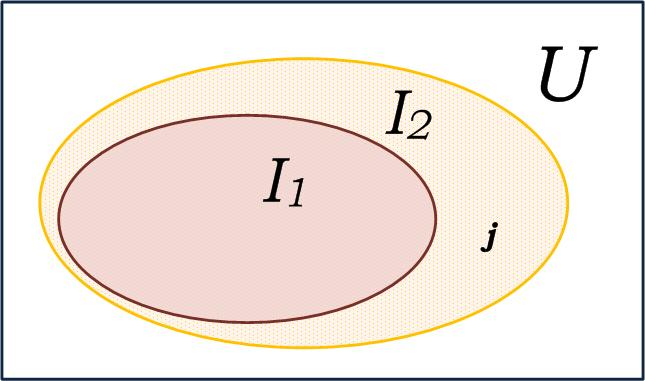
\includegraphics[width = 0.5\linewidth]{figures/subset.jpg}
	\vspace{10pt}
	\caption{增强层数据包集合关系示例 \label{fig:subset}}
\end{figure}

如果$I_1$是$I_2$的子集,那么二者的重建误差就可以由公式(\ref{eq:subset2})与(\ref{eq:subset1})相减得到:
\begin{equation}
\vspace{10pt}
\label{eq:minus1}
(s_{I_2} - s_{I_1}) = {\rm\bf M} \cdot (s_{I_2} - s_{I_1}) + \Big( \sum_{i \in I_2}{\rm\bf T}_i \cdot c_i - \sum_{i \in I_1}{\rm\bf T}_i \cdot c_i \Big) \: ,
\end{equation}
\begin{equation}
\vspace{10pt}
\label{eq:minus2}
\Rightarrow e = s_{I_2} - s_{I_1} = ({\rm\bf I - M})^{-1} \cdot \Big( \sum_{i \in I_2}{\rm\bf T}_i \cdot c_i - \sum_{i \in I_1}{\rm\bf T}_i \cdot c_i \Big) \: .
\end{equation}

特别地,如果$I_2$和$I_1$的差别只有一个增强层数据包$j$,也就是说$I_2 \setminus I_1 = \{j\}$(如图\ref{fig:subset}所示),那么根据公式(\ref{eq:minus2}),这两个重建序列的差为:
\begin{equation}
\vspace{10pt}
\label{eq:error_j}
e_j = ({\rm\bf I - M})^{-1} \cdot {\rm\bf T}_j \cdot c_j \: .
\end{equation}

可以看到,$e_j$只由数据包$j$决定,与其他的增强层数据包无关。这个值$e_j$被定义为数据包$j$的“误差向量”,表示丢弃数据包$j$后所带来的像素值误差。我们可以通过如下的方式得到任何一个数据包$j$的误差向量:选取两个只差$j$的数据包子集,将它们解码得到的视频序列相减即可。

一旦获取了所有增强层数据包对应的误差向量,那么丢弃任意一个增强层数据包子集所导致的失真就可以用这个子集中的数据包的误差向量之和来估计。举例来说,如果增强层数据包$x$, $y$, $z$从一个码流中被丢弃,那么丢弃前后的重建序列之差应该为:
\begin{equation}
\vspace{10pt}
e = e_x + e_y + e_z.
\end{equation}
这个简单的相加之所以合理有两方面的原因。第一,不像MSE或PSNR,误差向量仅仅是像素的差值,并不涉及二次方运算。第二,每个增强层数据包在重建中会各自对像素进行精细化,其效果是叠加的(参见前面的推导过程)。

应该指出,上述第二点原因的成立是有条件的。在公式(\ref{eq:base0})到(\ref{eq:subset2})中,${\rm\bf M}$和$p$的值都相同是因为,在质量可伸缩的情况下,增强层数据包仅仅是通过操作变换系数得到的,并不涉及运动校正和静态预测过程。然而这对于其他维度的可伸缩(例如视频分辨率改变的空间可伸缩)并不正确。因此,此处推导的线性误差模型并不适用于任意配置的可伸缩视频编码。在本文的研究中,只用到了质量可伸缩;其他伸缩维度将作为未来工作中的探索对象。

\subsection{误差向量获取}

如果按照上一小节中所说,每次计算一个数据包的误差向量,那么所需的解码次数将是所有数据包的个数。这么做的计算量太大。在本小节中,我们给出一个高效获取所有误差向量的方法。

\begin{figure}[h]
\centering
\vspace{10pt}
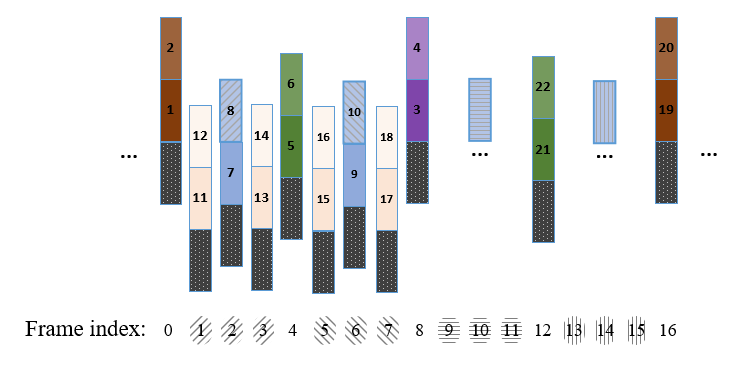
\includegraphics[width = 1.0\linewidth]{figures/GOP-structure.png}
\caption{SVC码流中的图像组(GOP)结构示例 \label{fig:GOP-structure}}
\end{figure}

为了减少解码次数,我们将所有的增强层数据包分成若干组,使得每一组中的多个误差向量能在一次解码中同时获取。考虑如图\ref{fig:GOP-structure}所示具有8帧图像组结构的一个视频码流。在该图中,基本层数据包是黑色的,增强层数据包按照颜色分为了几个组(相同颜色的属于同一组)。在每一组中,增强层数据包的误差向量可以同时计算,因为这些数据包所影响的像素是互不干扰的。例如,丢弃8号数据包只会在帧1、2、3中带来像素误差,而丢弃10号数据包只会在帧5、6、7中带来像素误差(帧的编号从0开始)。因此,我们可以只通过一次相减来同时得到8号和10号数据包的误差向量$e_{8}$和$e_{10}$,以及所有其他GOP中的相同位置数据包(用相同颜色表示它们属于同一组)的误差向量。应该指出,这些误差向量是非常稀疏的,因为丢弃单个数据包带来的失真影响非常有限。

为了获取所有的误差向量,所需的解码次数大约等于增强层的层数$(L_Q - 1)$乘以时间层的层数$L_T$。对于图\ref{fig:GOP-structure}中的例子而言,$L_Q = 3$,$L_T = 4$,所以所需的解码次数照此计算将会是$(3 - 1) \times 4 = 8$。然而,我们还需要额外的$L_Q - 1 = 2$次解码,来分离“关键帧”\supercite{H.264-Overview}(图\ref{fig:GOP-structure}中的帧0、8、16)中数据包的失真影响。关键帧中增强层数据包的丢弃将会给它两边相邻的两个GOP都带来失真。例如,丢弃4号数据包带来的失真影响范围将会从帧1直到帧15,从而与帧0和帧16中的数据包的失真影响互相交叠。因此,关键帧同一位置的增强层数据包(2、4、20号数据包)应该被分为两个组:一组包含偶数GOP的关键帧数据包(2和20号包),另一组包含奇数GOP的(4号包)。于是,误差向量获取真正所需要的解码次数应为:
\begin{equation}
\vspace{10pt}
N = (L_Q - 1) \cdot (L_T + 1).
\end{equation}
这与JSVM中Quality Layer信息的获取所需的解码次数大致相当。

\subsection{失真估计与模型验证}
\vspace{10pt}
\label{subsec:distortion-estimation}

基于线性误差模型,我们可以估计丢弃任意增强层数据包组合带来的失真,只需把所丢弃的每一个数据包对应的误差向量加起来即可。

例如,对于一个通过丢弃数据包集合$I_x$而得到的子流来说,它解码出来的视频序列与原始序列间的差值可以估计为:
\begin{equation}
\vspace{10pt}
\label{eq:subset_error}
e(I_x) = e_{full} + \sum_{i \in {I_x}} e_i \: .
\end{equation}
这个公式中$e_{full}$表示全部增强层数据包都参与解码得到的视频序列与原始序列之间的差值。这是编解码过程固有的失真,在一个数据包都不丢弃的时候也是存在的。

在采用基于线性误差模型的失真估计之前,我们先做实验验证一下其准确性。该实验中的码流都是用JSVM编码器压缩得到的,编码采用了如图\ref{fig:GOP-structure}所示的GOP结构,熵编码过程配置的是CABAC。每个码流基本层和增强层的QP分别为33和27。增强层通过配置Medium Grain Scalability (MGS)向量进一步划分为了2个MGS层,分别包含4个和12个变换系数。我们从码流中随机丢弃一组数据包,将得到的子流解码,然后比较实际的失真与通过线性误差模型估计的失真。解码用的是JSVM解码器,其他计算都通过MATLAB进行。

对于序列{\em Bus}、{\em Foreman}、{\em Soccer},图\ref{fig:model-verification}分别给出了其中一个比较结果(为简单起见,只采用了前33帧)。图中的横轴代表帧序号,纵轴表示以MSE度量的失真。实线代表真实计算的失真,虚线代表用所提出的线性误差模型估计的失真。可以看到虚线和实线非常接近,验证了用提出的模型做失真估计的准确性。我们对所有8个SVC标准序列都进行了实验,定量计算了估计误差,如表\ref{tab:estimation-error}所示。可以看到,平均估计误差只有5\%,进一步说明了模型的准确性。


\begin{figure}[!ht]
	\centering
	\subfloat[{\em Bus}]{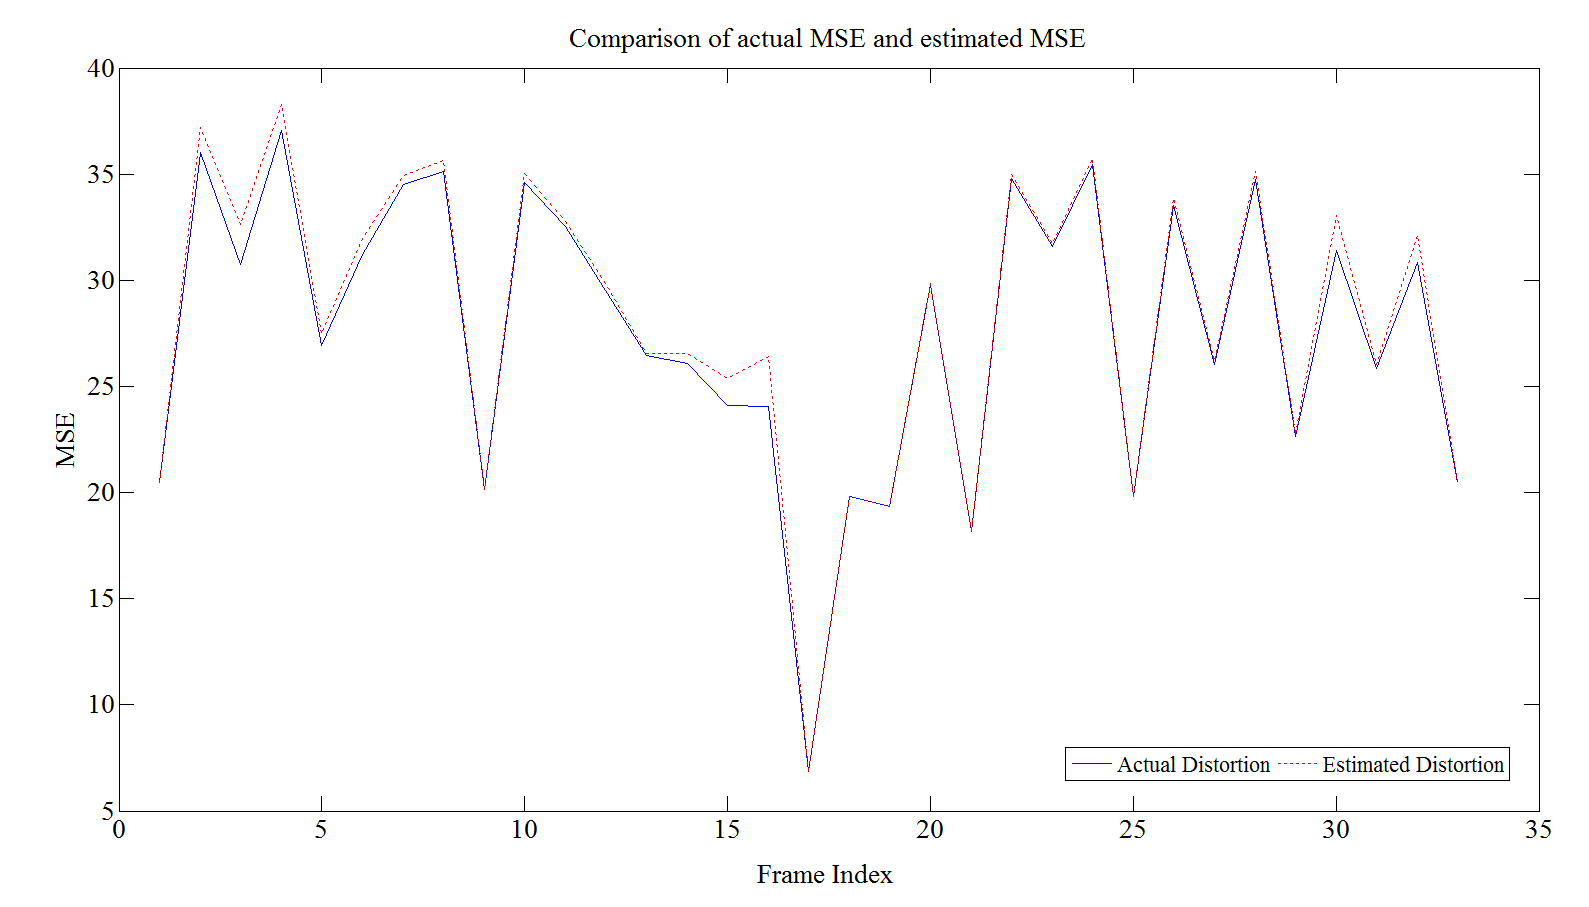
\includegraphics[width=0.7\textwidth]{figures/model-verify-Bus.png}} \\
	\subfloat[{\em Foreman}]{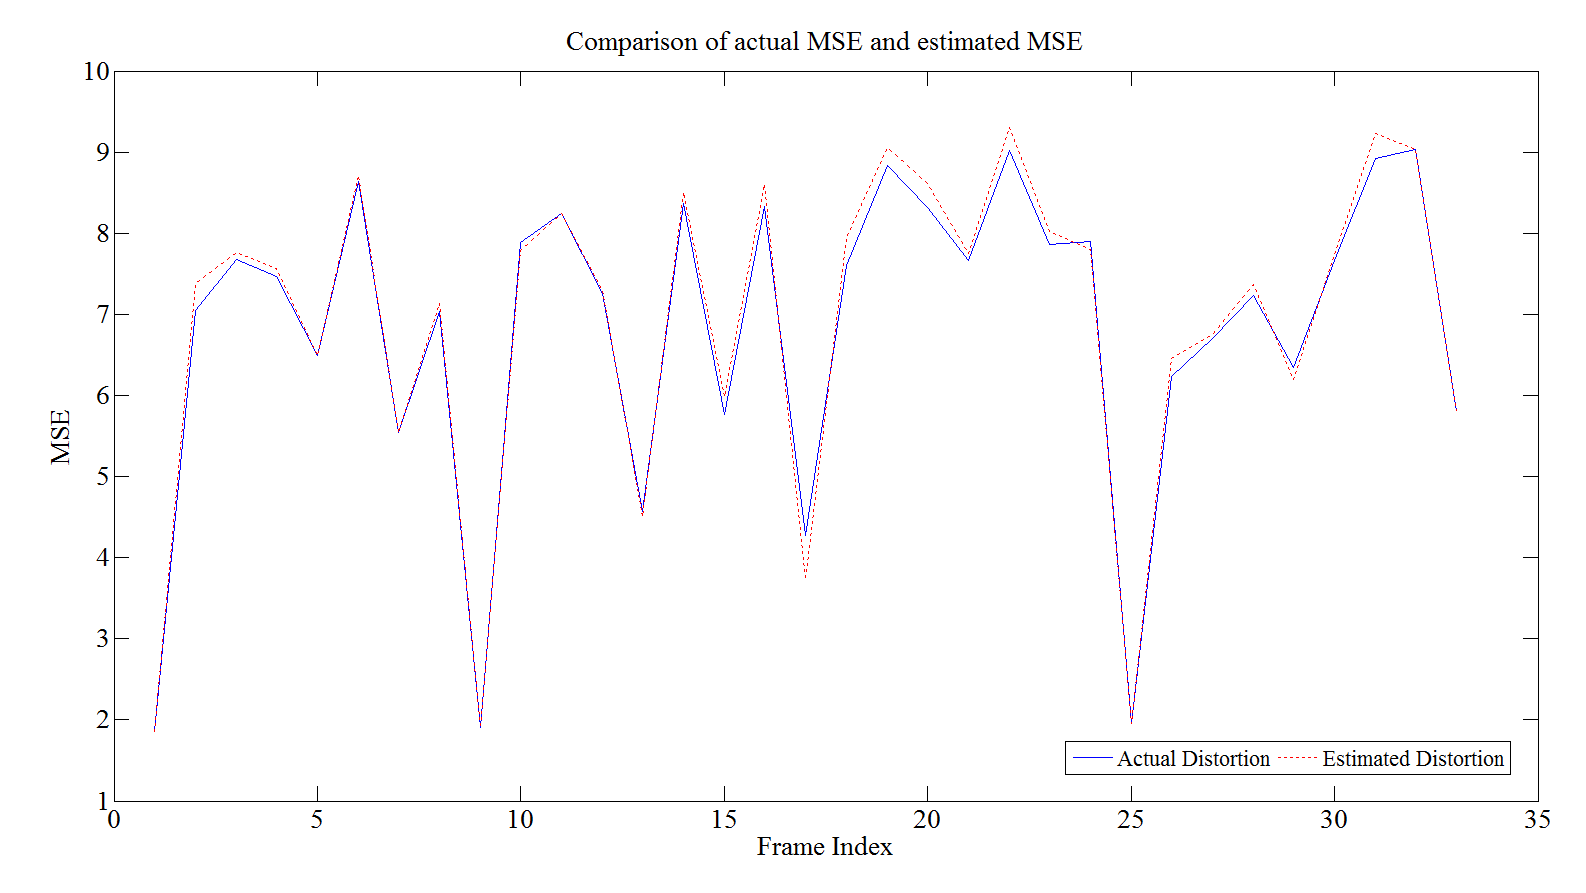
\includegraphics[width=0.7\textwidth]{figures/model-verify-Foreman.png}} \\
	\subfloat[{\em Soccer}]{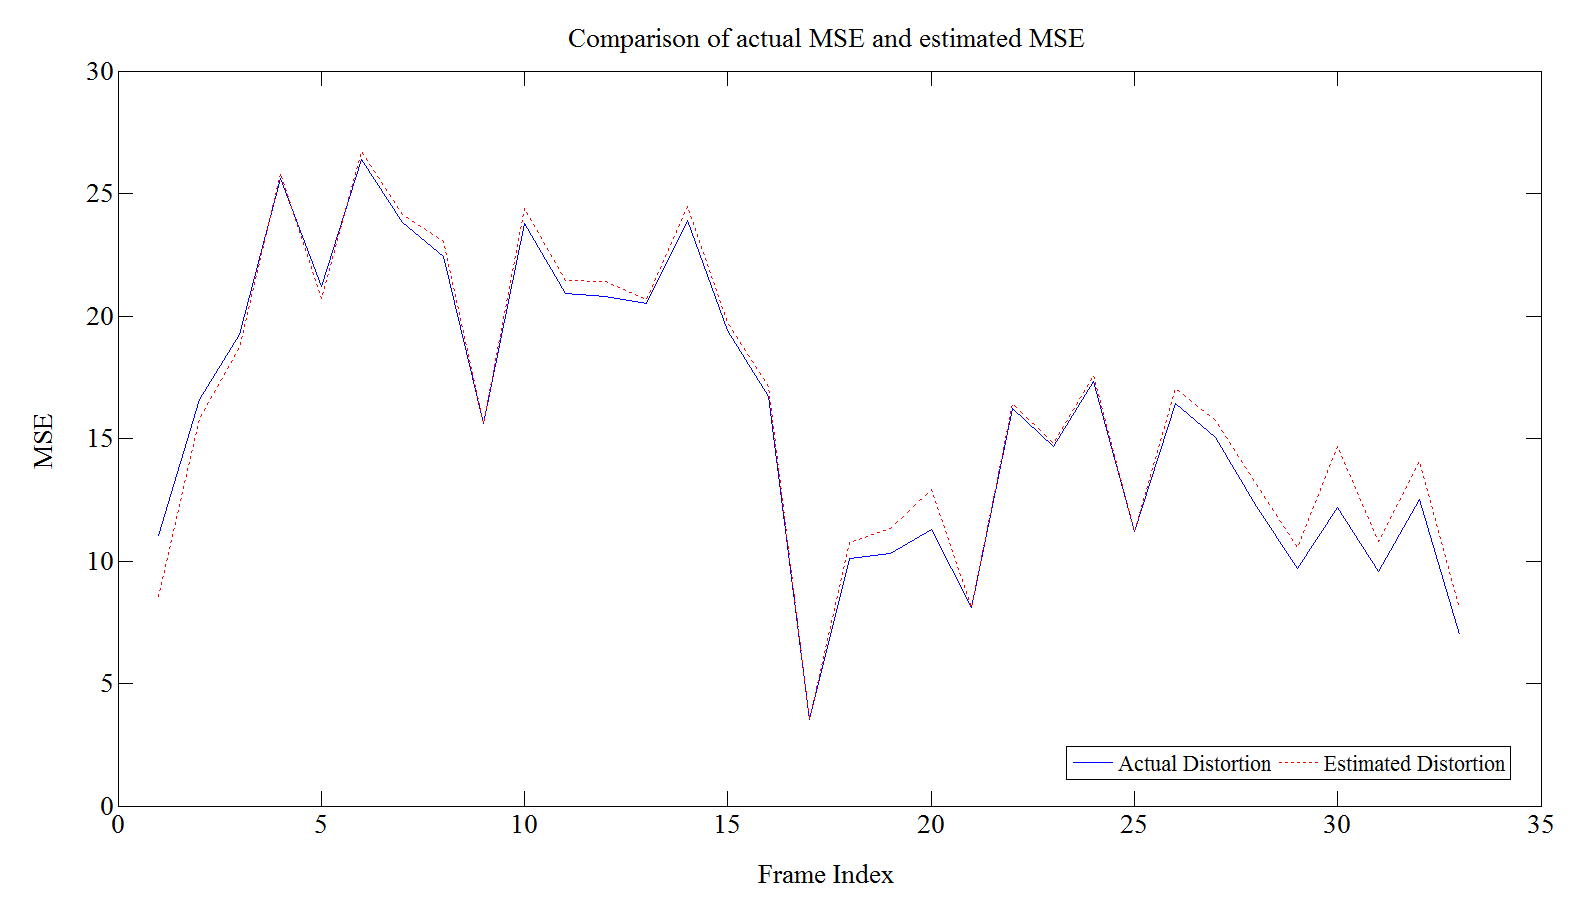
\includegraphics[width=0.7\textwidth]{figures/model-verify-Soccer.png}} \\
	\caption{不同序列估计失真与实际失真的比较 \label{fig:model-verification}}
\end{figure}

\begin{table}[h]
	\centering
	\vspace{10pt}
	\caption{采用线性误差模型进行不同序列失真估计的估计误差}
	\label{tab:estimation-error}
	\begin{tabular}{*{8}{p{1.35cm}<{\centering}|}{p{1.3cm}<{\centering}}}
		\hline\hline
		{\em Bus} & {\em City} & {\em Crew} & {\em Football} & {\em Foreman} & {\em Harbour} & {\em Mobile} & {\em Soccer} & \textbf{Average} \\ \hline
		2.83\% & 2.39\% & 10.36\% & 7.08\% & 4.95\% & 2.63\% & 5.77\% & 5.26\% & \textbf{5.16\%} \\ \hline
	\end{tabular}
\end{table}

\section{码流截取方案}
\label{extraction}

在这一节中,我们采用上面提出的线性误差模型来进行码流截取。因为找到码流截取问题的最优解不太现实,我们的方案采用贪心法\footnote{https://en.wikipedia.org/wiki/Greedy\_algorithm}来获得一个次优解。与“0-1背包问题”的贪心解法类似,每次当一个数据包需要被丢弃时,我们选择具有最小的码率失真影响的包。一个包的码率失真影响可以被认为决定它是否重要的优先级度量标准。下面我们首先对所采用的这个度量标准做简单的介绍,然后具体给出优先级赋值的算法。

\subsection{数据包优先级度量}

对于一个数据包,我们采用如下的码率失真影响来度量它的优先级:
\begin{equation}
\vspace{10pt}
\label{eq:rd_impact}
\Phi = \dfrac{\partial D}{\partial R} \: ,
\end{equation}
其中$\partial D$表示丢弃这个数据包所带来的失真的变化,而$\partial R$是相应的码率的变化。$\partial R$显然只与该数据包本身的大小有关,很容易得到。但$\partial D$的真实值需要通过分别计算丢包前后的失真来求取,在码流截取中只能估计。

这一度量标准具有直观上的意义。如果丢弃了一个数据包之后所带来的码率变化很小($\partial R$小),而丢掉它产生的失真变化却很大($\partial D$大),那意味着这个数据包非常重要,其优先级高($\Phi$大),在码流截取中应该尽量予以保留。这样的数据包本身没有很多数据,但它所处的帧被较多的其他帧所参考,丢弃之后具有较大的失真影响。采用公式(\ref{eq:rd_impact})所示的度量标准能够全面考虑到这种情形。

\subsection{优先级赋值的贪心算法}
\label{subsec:priority-assign}

我们将模拟依次从一个码流中丢掉所有增强层数据包的过程,丢包顺序就按照上面所说的贪心策略。这个顺序就作为数据包的优先级值被记录下来。这些优先级值可以被存储在码流中(NALU头信息的优先级ID字段或者补充增强信息SEI中),用于实际的码流截取。本节详细介绍优先级赋值的算法。

对于很长的视频序列,往往将其分为一个个优化窗口进行操作。每个窗口含有一定数量的帧,优先级赋值和码流截取都在每个窗口中独立地进行。假设优化窗口的长度为$K$,也就是说每次处理$K$帧;再假设每一帧包含的质量伸缩层个数为$L_Q$,也就是一个基本层加$L_Q-1$个增强层。这样的话所有能够被丢弃的增强层数据包的个数将是$K \cdot (L_Q-1)$。在每一次贪心选择的步骤中,当前可以被丢弃的数据包只能是每一帧最上层的数据包(因为下层的包被上层所依赖),也就是最多有$K$个。在这样的优化窗口中进行优先级赋值的过程具体描述如下:

\begin{description}
	\vspace{10pt}
	\item[1)] 初始状态下,把整个序列的误差向量$e_{seq}$设为$e_{full}$(所有增强层数据包都在时解码出的序列与原始序列的差值,参见公式(\ref{eq:subset_error})的说明)。
	\vspace{10pt}
	\item[2)] 在所有当前可以丢弃的数据包中,找到对序列具有最小码率失真影响的数据包$m$,即寻找$m$,使得:
	\begin{equation}
	\vspace{10pt}
	\label{eq:R-D_impact_m}
	\Phi_m = \min_{i \in I_{top}} \Phi_i \: ,
	\end{equation}
	其中$I_{top}$代表当前处于每一帧最上层的数据包,现在只有它们是可以丢弃的。一个包的失真影响基于公式(\ref{eq:rd_impact})计算如下: 
	\vspace{10pt}
	\begin{equation}
	\vspace{10pt}
	\label{eq:R-D_impact_i}
	\Phi_i = \dfrac{\partial D}{\partial R} = \dfrac{PSNR(e_{seq}) - PSNR(e_{seq} + e_i)}{SIZE(i)} \: ,
	\end{equation}
	其中$SIZE(i)$是数据包$i$的大小,$PSNR(*)$是由误差向量求取PSNR的函数。PSNR是由MSE定义的,而MSE就是误差向量的元素平方后的均值。
	\vspace{10pt}
	\item[3)]将数据包$m$从码流中移除,并把它的误差向量加到序列误差向量中:
	\begin{equation}
	\label{eq:error_update}
	e_{seq} = e_{seq} + e_m \: .
	\end{equation}
	\item[4)]重复2)到3)的步骤,直到所有的增强层数据包全部被移除,且每个包都根据它被移除的次序被赋予了优先级值。
	\vspace{10pt}
\end{description}

上面描述的过程用算法伪码表示可参见Algorithm\ref{algo:greedy}。

\begin{algorithm}
	\caption{优先级赋值的贪心算法}
	\label{algo:greedy}
	\begin{algorithmic}
		\STATE 初始化$e_{seq}$为$e_{full}$, 初始化$q$为0;
		\WHILE{$q < K \cdot (L_Q - 1)$}
		\FOR{(最多)$K$个处于每帧最上层的数据包}
		\STATE 找到具有最小失真影响$\Phi_m$的数据包$m$;
		\ENDFOR
		\STATE 设置$m$的优先级为$q$;
		\STATE 将$m$从码流中移除;
		\STATE 将$e_{seq}$更新为$e_{seq} + e_m$,并将$q$更新为$q+1$;
		\ENDWHILE
	\end{algorithmic}
\end{algorithm}

从伪码很容易看出优先级赋值算法的时间复杂度为$O(K^2)$。需要指出的是,在优先级赋值过程中的这些计算量相比于误差向量获取过程中解码的计算量来说是微不足道的。通过增加优化窗口大小$K$,可以每次比较更多的数据包来确定优先级,因此有望得到更优的截取结果。然而,这样做不仅增加计算量,更重要的是会使存储误差向量所需的内存有显著的增加。此外,如果优先级值采用NALU头信息中的字段存储的话,因为该字段只有6个比特,所支持的范围是0~63,这也限制了$K$的大小。

\subsection{无参考源的情况}
\label{subsec:noref}

在某些场合,优先级赋值和码流截取需要在没有原始视频序列的情况下进行。这将增加问题的难度,因为当原始序列未知的时候更难以获取实际失真。这种无参考的情形在实际中甚至比有参考的情形更常见。因为通常来说,流媒体服务提供商拿到的都是压缩后的码流,很少能拿到原始视频序列。在这一小节中,我们对所提出的算法稍作修改以适应这种没有参考源的特殊情况。

在缺少原始序列的情况下,我们无法计算上面提到的$e_{full}$。一个简单直接的想法是把$e_{full}$置为0,也就是所有失真都是基于整个码流完全重建的像素来计算,而不是基于原始序列。但我们发现这样做效果并不好,算法过程中的PSNR值太大,无法很好的反映实际失真。这是因为丢弃一些数据包后,与完全重建像素比较起来并不能带来很大的误差,据此计算PSNR是不合适的。为了解决这个问题,我们改为直接用所有像素的均方差(MSE)作为失真的度量标准,不再计算PSNR。即,公式(\ref{eq:R-D_impact_i})应修改为:
\vspace{10pt}
\begin{equation}
\vspace{10pt}
\label{eq:R-D_impact_i_noref}
\Phi_i = \dfrac{\partial D}{\partial R} = \dfrac{MSE(e_{seq}) - MSE(e_{seq} + e_i)}{SIZE(i)} \: ,
\end{equation}
其中,$MSE(*)$表示直接由误差向量得到MSE。这样做使得无参考情况下的截取效果有所提升,被证明是一个合理有效的改进(参见下一节中的相应实验结果)。

\subsection{优先级值的实际使用}

上面所述的算法为可伸缩视频码流中的每个增强层数据包赋予了一个优先级值,这些优先级值将用于实际的码流截取。本小结具体介绍在实际系统中如何使用优先级值来进行码流截取。

首先,系统应该提前确定每个优先级值与码率的对应关系,这只需要进行一次性的统计操作。有了这个对应关系之后,在给定的截取码率下,就知道了应保留的数据包优先级下限。假设这个下限为P,则在传输时,所有增强层数据包优先级低于P的都应该丢弃。在发送一个数据包前,传输程序首先检查它是基本层数据包还是增强层数据包。如果是前者,则发送;如果是后者,则读取其优先级值与P比较。如果大于等于P,则发送;如果小于P,则将其丢弃。

在我们所实现的支持可伸缩视频的达尔文流媒体服务器中,传输时每次发送的是一个RTP包,而一个RTP包中可能包含多个或者不到一个SVC数据包,即NALU(参见\ref{subsec:protocols}小节)。考虑到这一点,服务器程序应该按照如图\ref{fig:extraction-flow}所示的流程来实现发送前的码流截取。

\begin{figure}[!ht]
	\centering
	\vspace{10pt}
	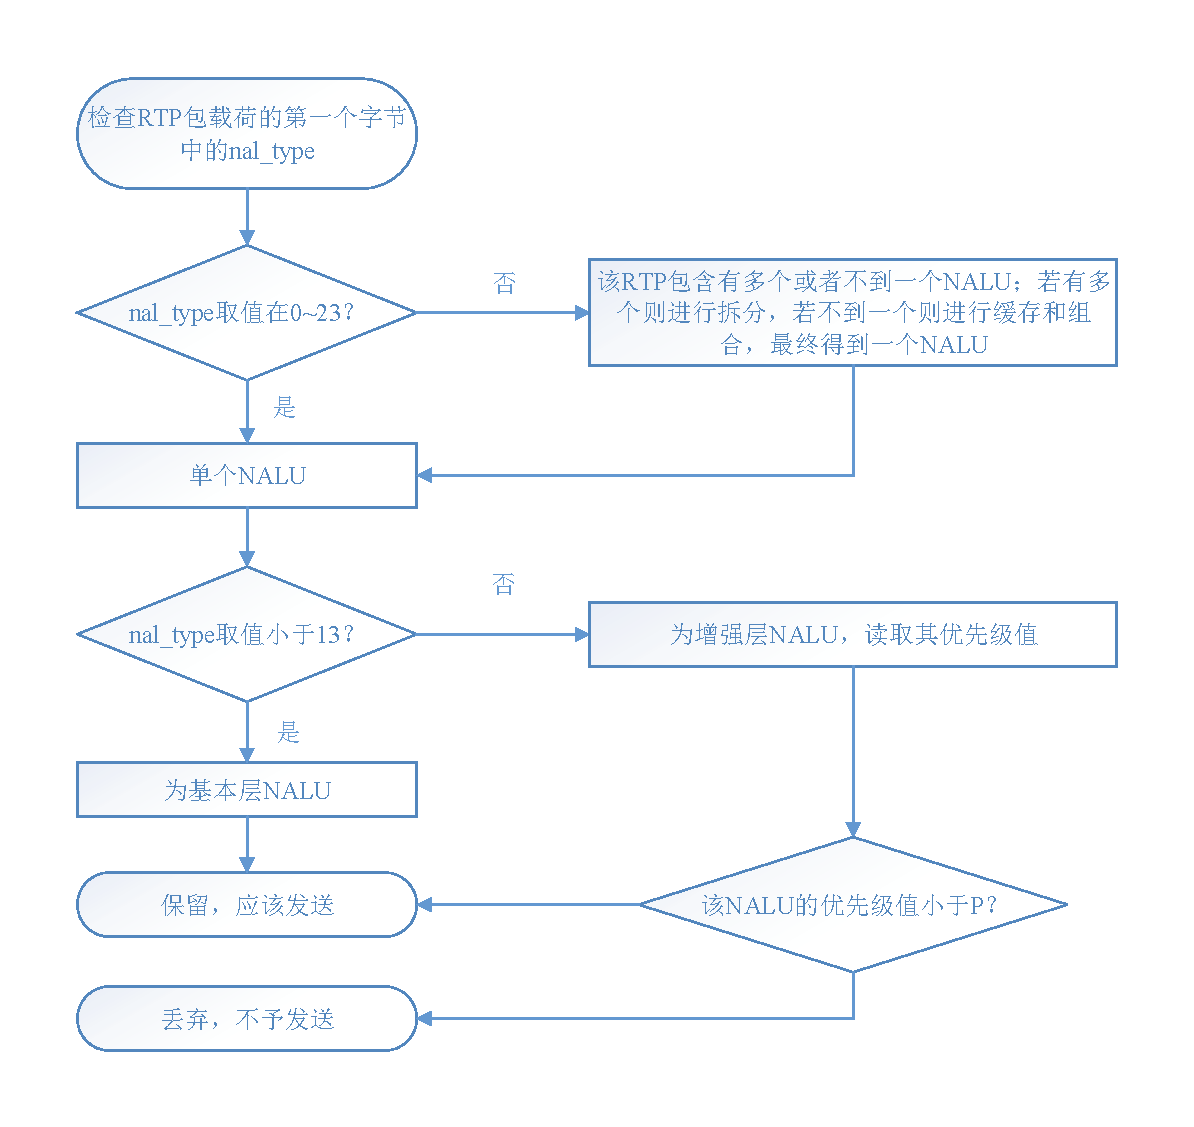
\includegraphics[width = 1.0\linewidth]{eps/extraction-flow}
	\caption{使用优先级值进行实际码流截取的程序流程图\label{fig:extraction-flow}}
	\vspace{10pt}
\end{figure}

\section{实验结果}

本节通过与参考软件JSVM(9.16版本)的对比来展示所提出的码流截取方案的实验结果。

\subsection{实验配置}

所有的测试码流都是按照\ref{subsec:distortion-estimation}中模型验证时所述的配置编码得到的。对于每个码流,我们选取十个截取点:一个是包含所有增强层数据包的完整码流,一个是只含有基本层数据包的最低码率码流,二者之间又等距离地选取了8个码率点。对每个码率点,我们用三种方法进行截取:JSVM中的基本截取器(用JSVM Basic指代),JSVM中采用了Quality Layers的截取器(用JSVM QL指代),以及本文提出的截取器。在本文提出的截取方案中,优先级赋值算法里的优化窗口大小是32帧,也就是4个GOP(GOP大小是8)。所有CIF大小的SVC标准测试序列都进行了测试,码率计算时采用了30FPS的帧率。

\subsection{结果分析}

\begin{figure*}[!ht]
	\centering
	\subfloat[Bus]{
		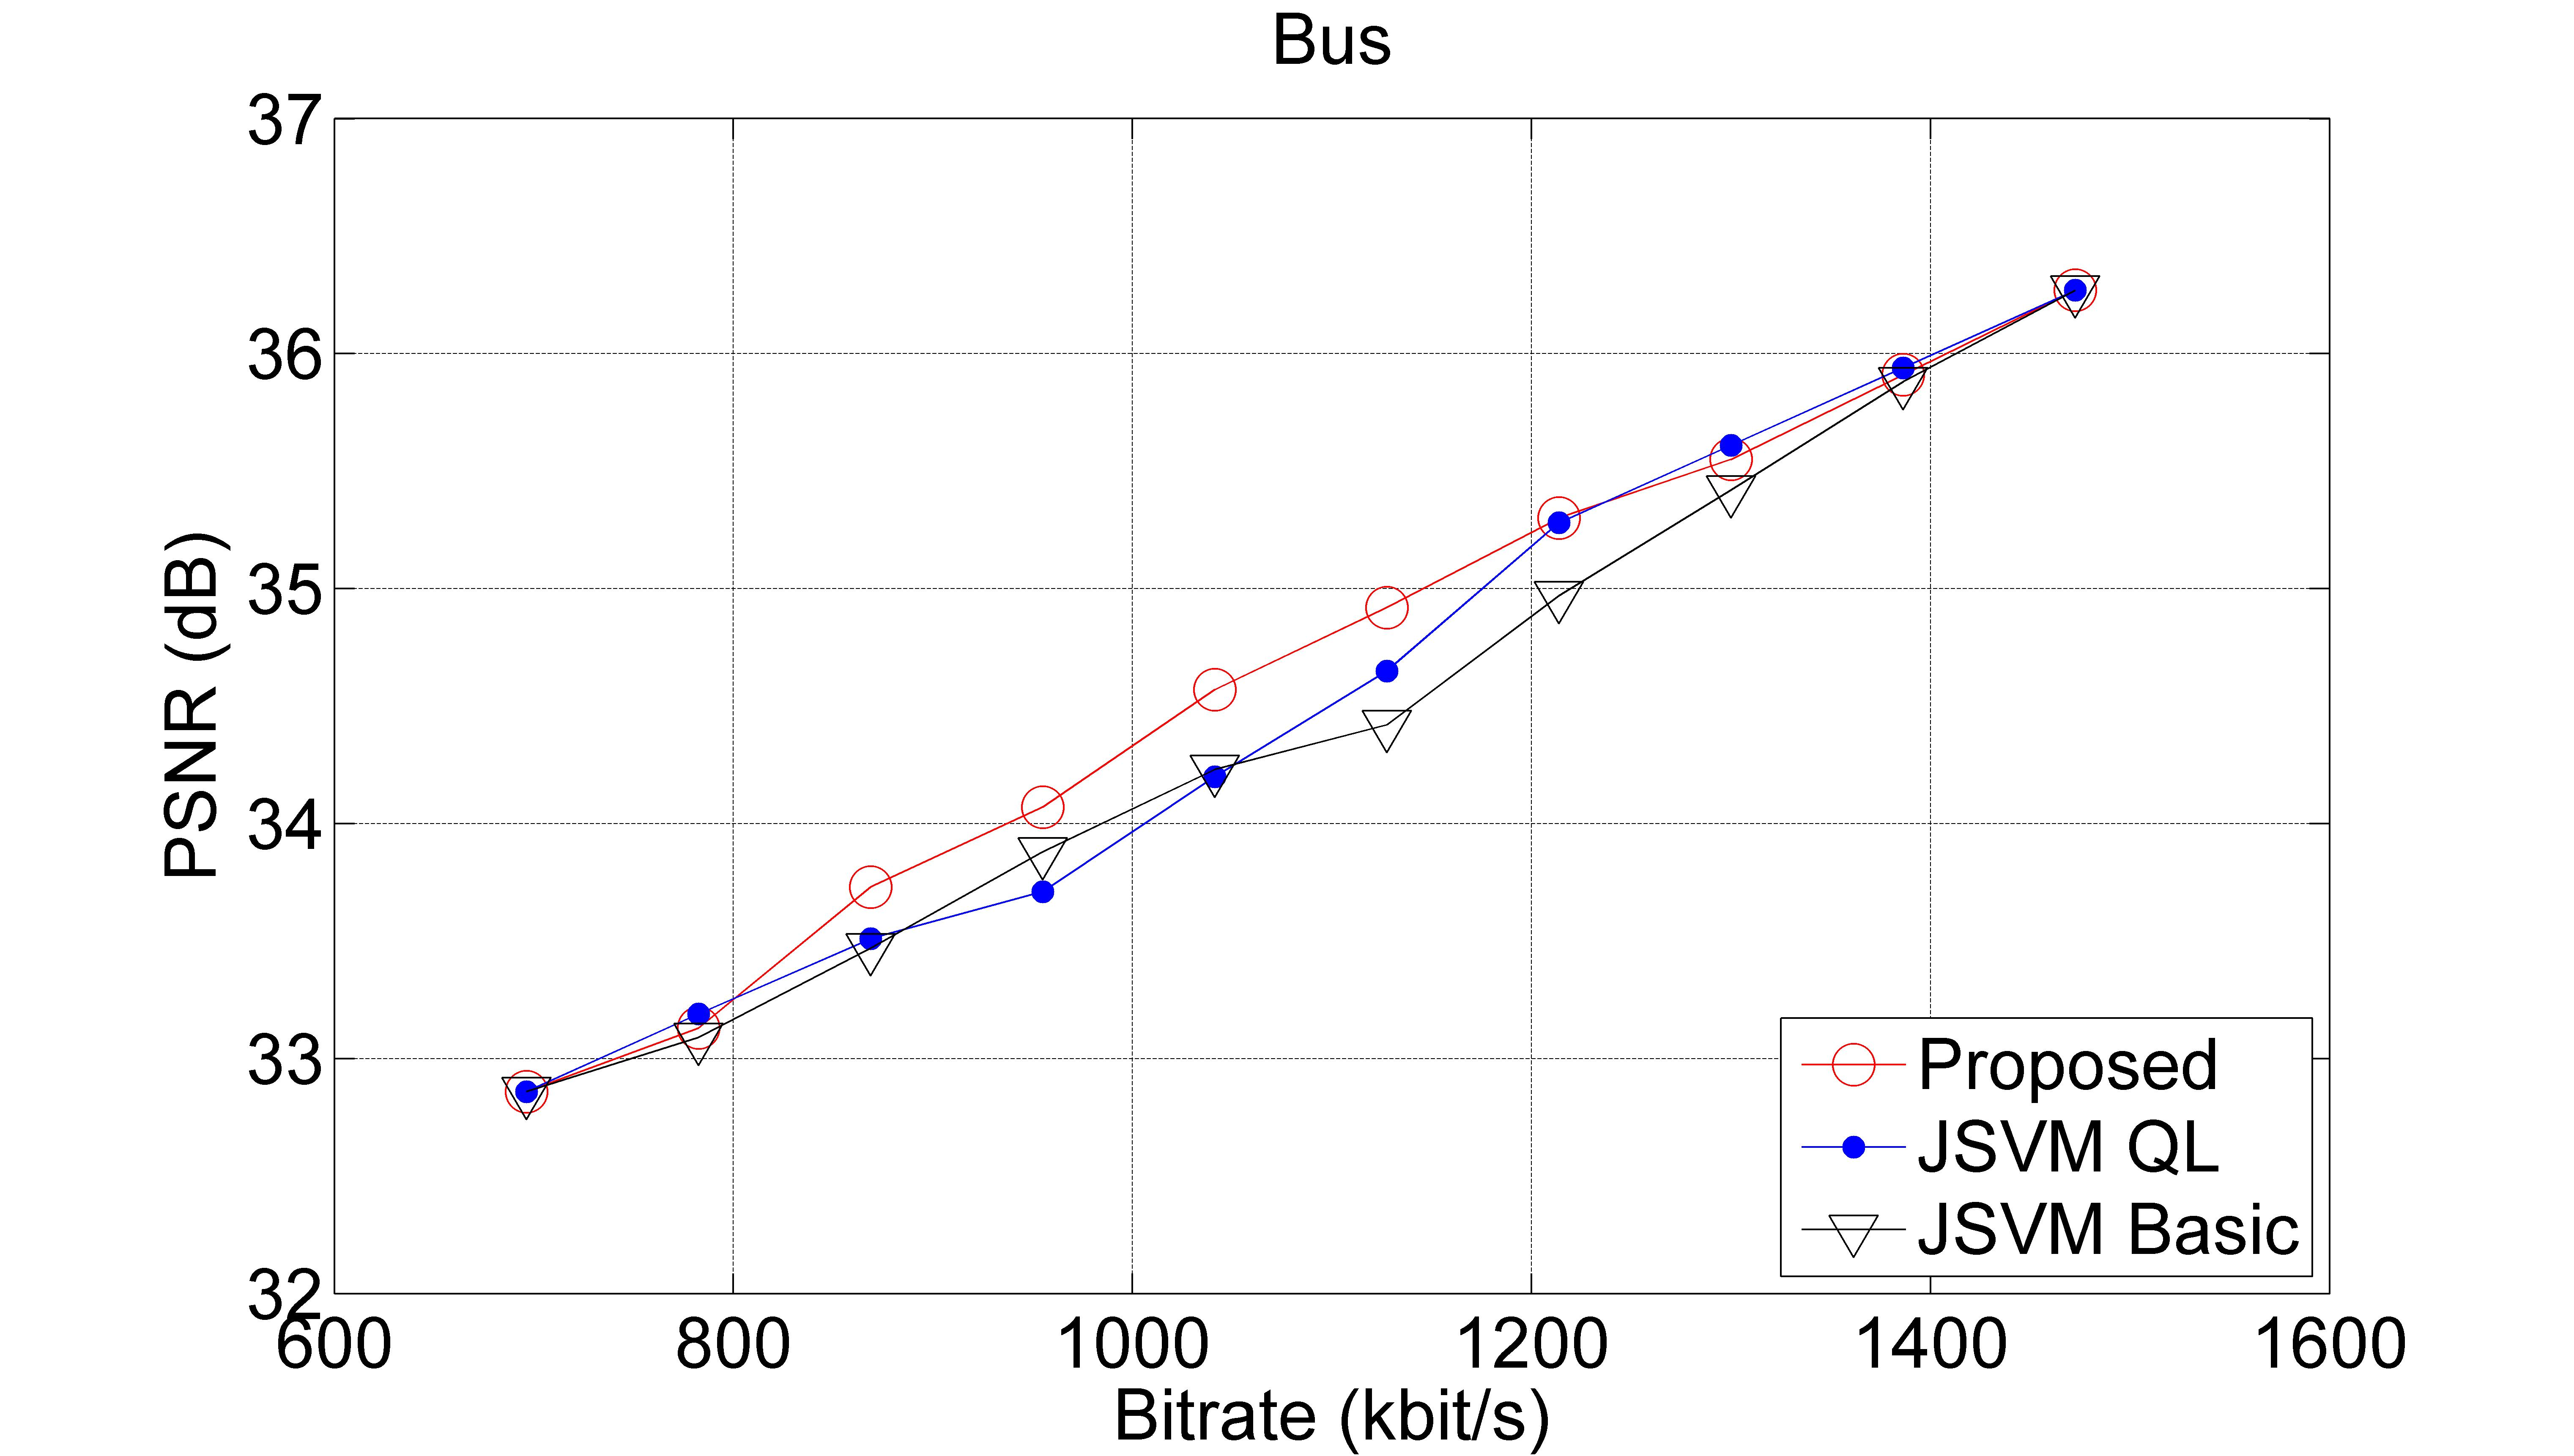
\includegraphics[width=0.5\textwidth]{figures/Bus.jpg}
		\label{fig:Bus}}
	\subfloat[City]{
		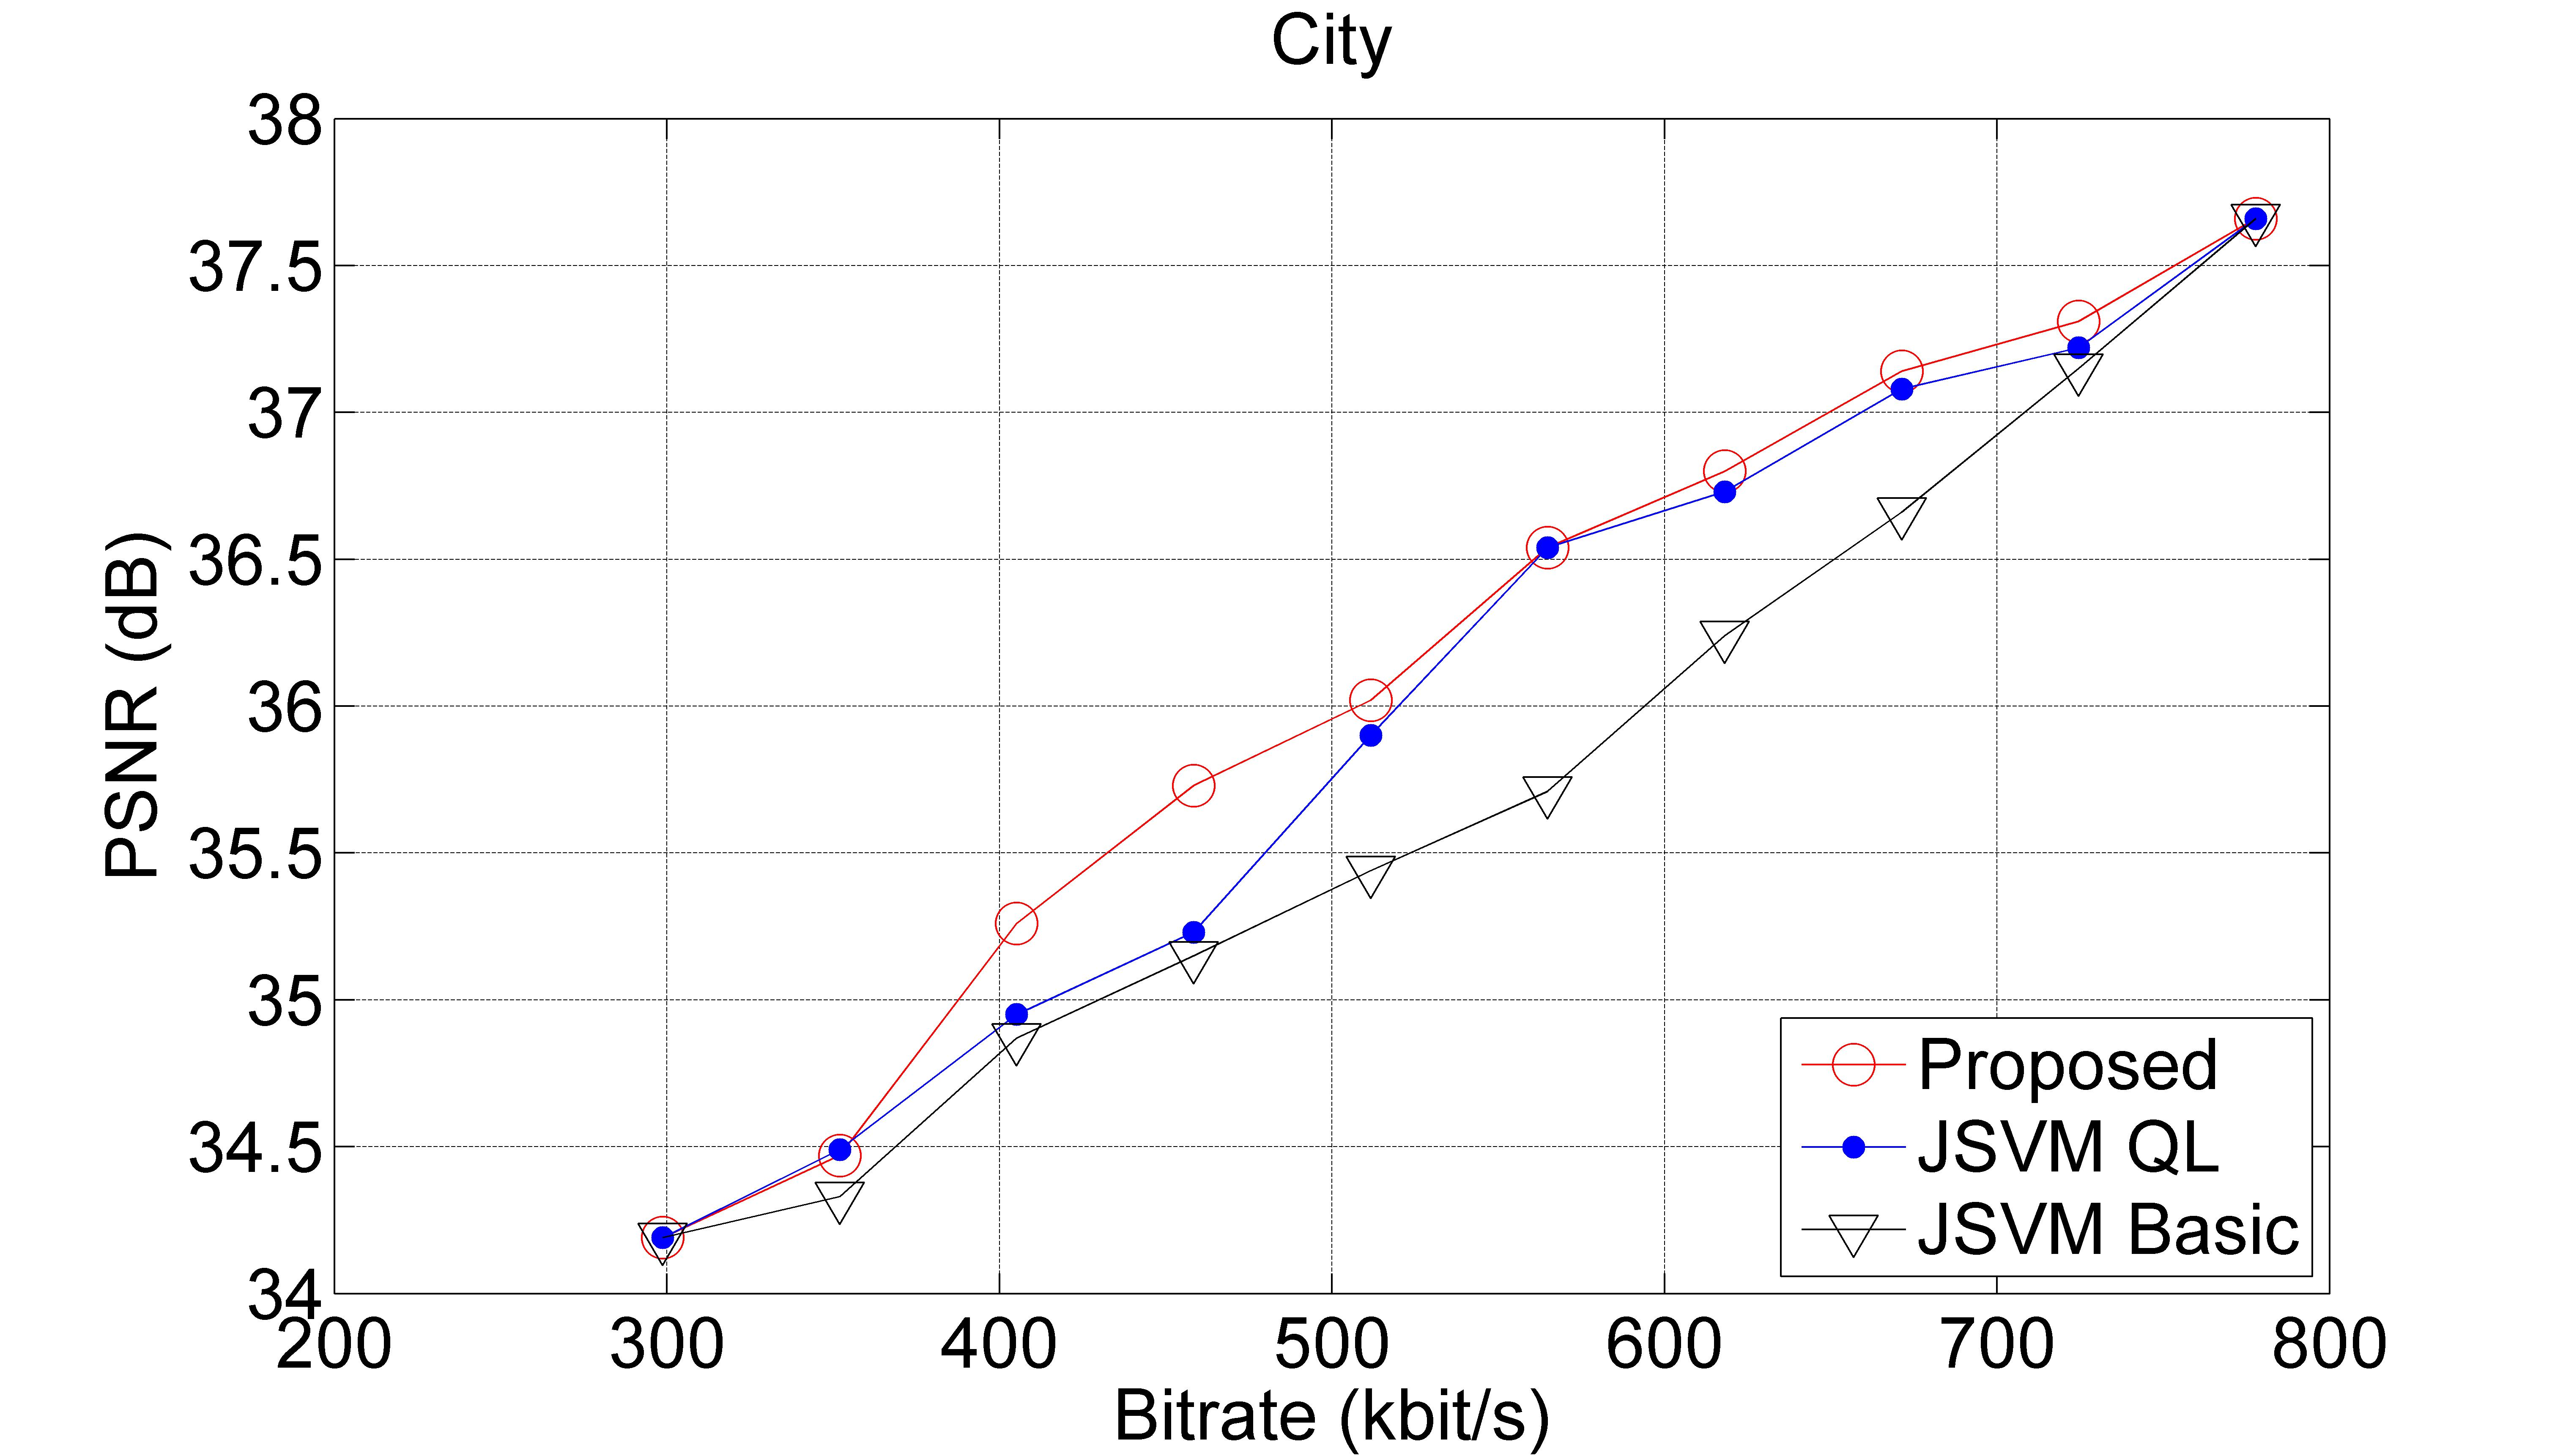
\includegraphics[width=0.5\textwidth]{figures/City.jpg}
		\label{fig:City}}
	\qquad
	\subfloat[Crew]{
		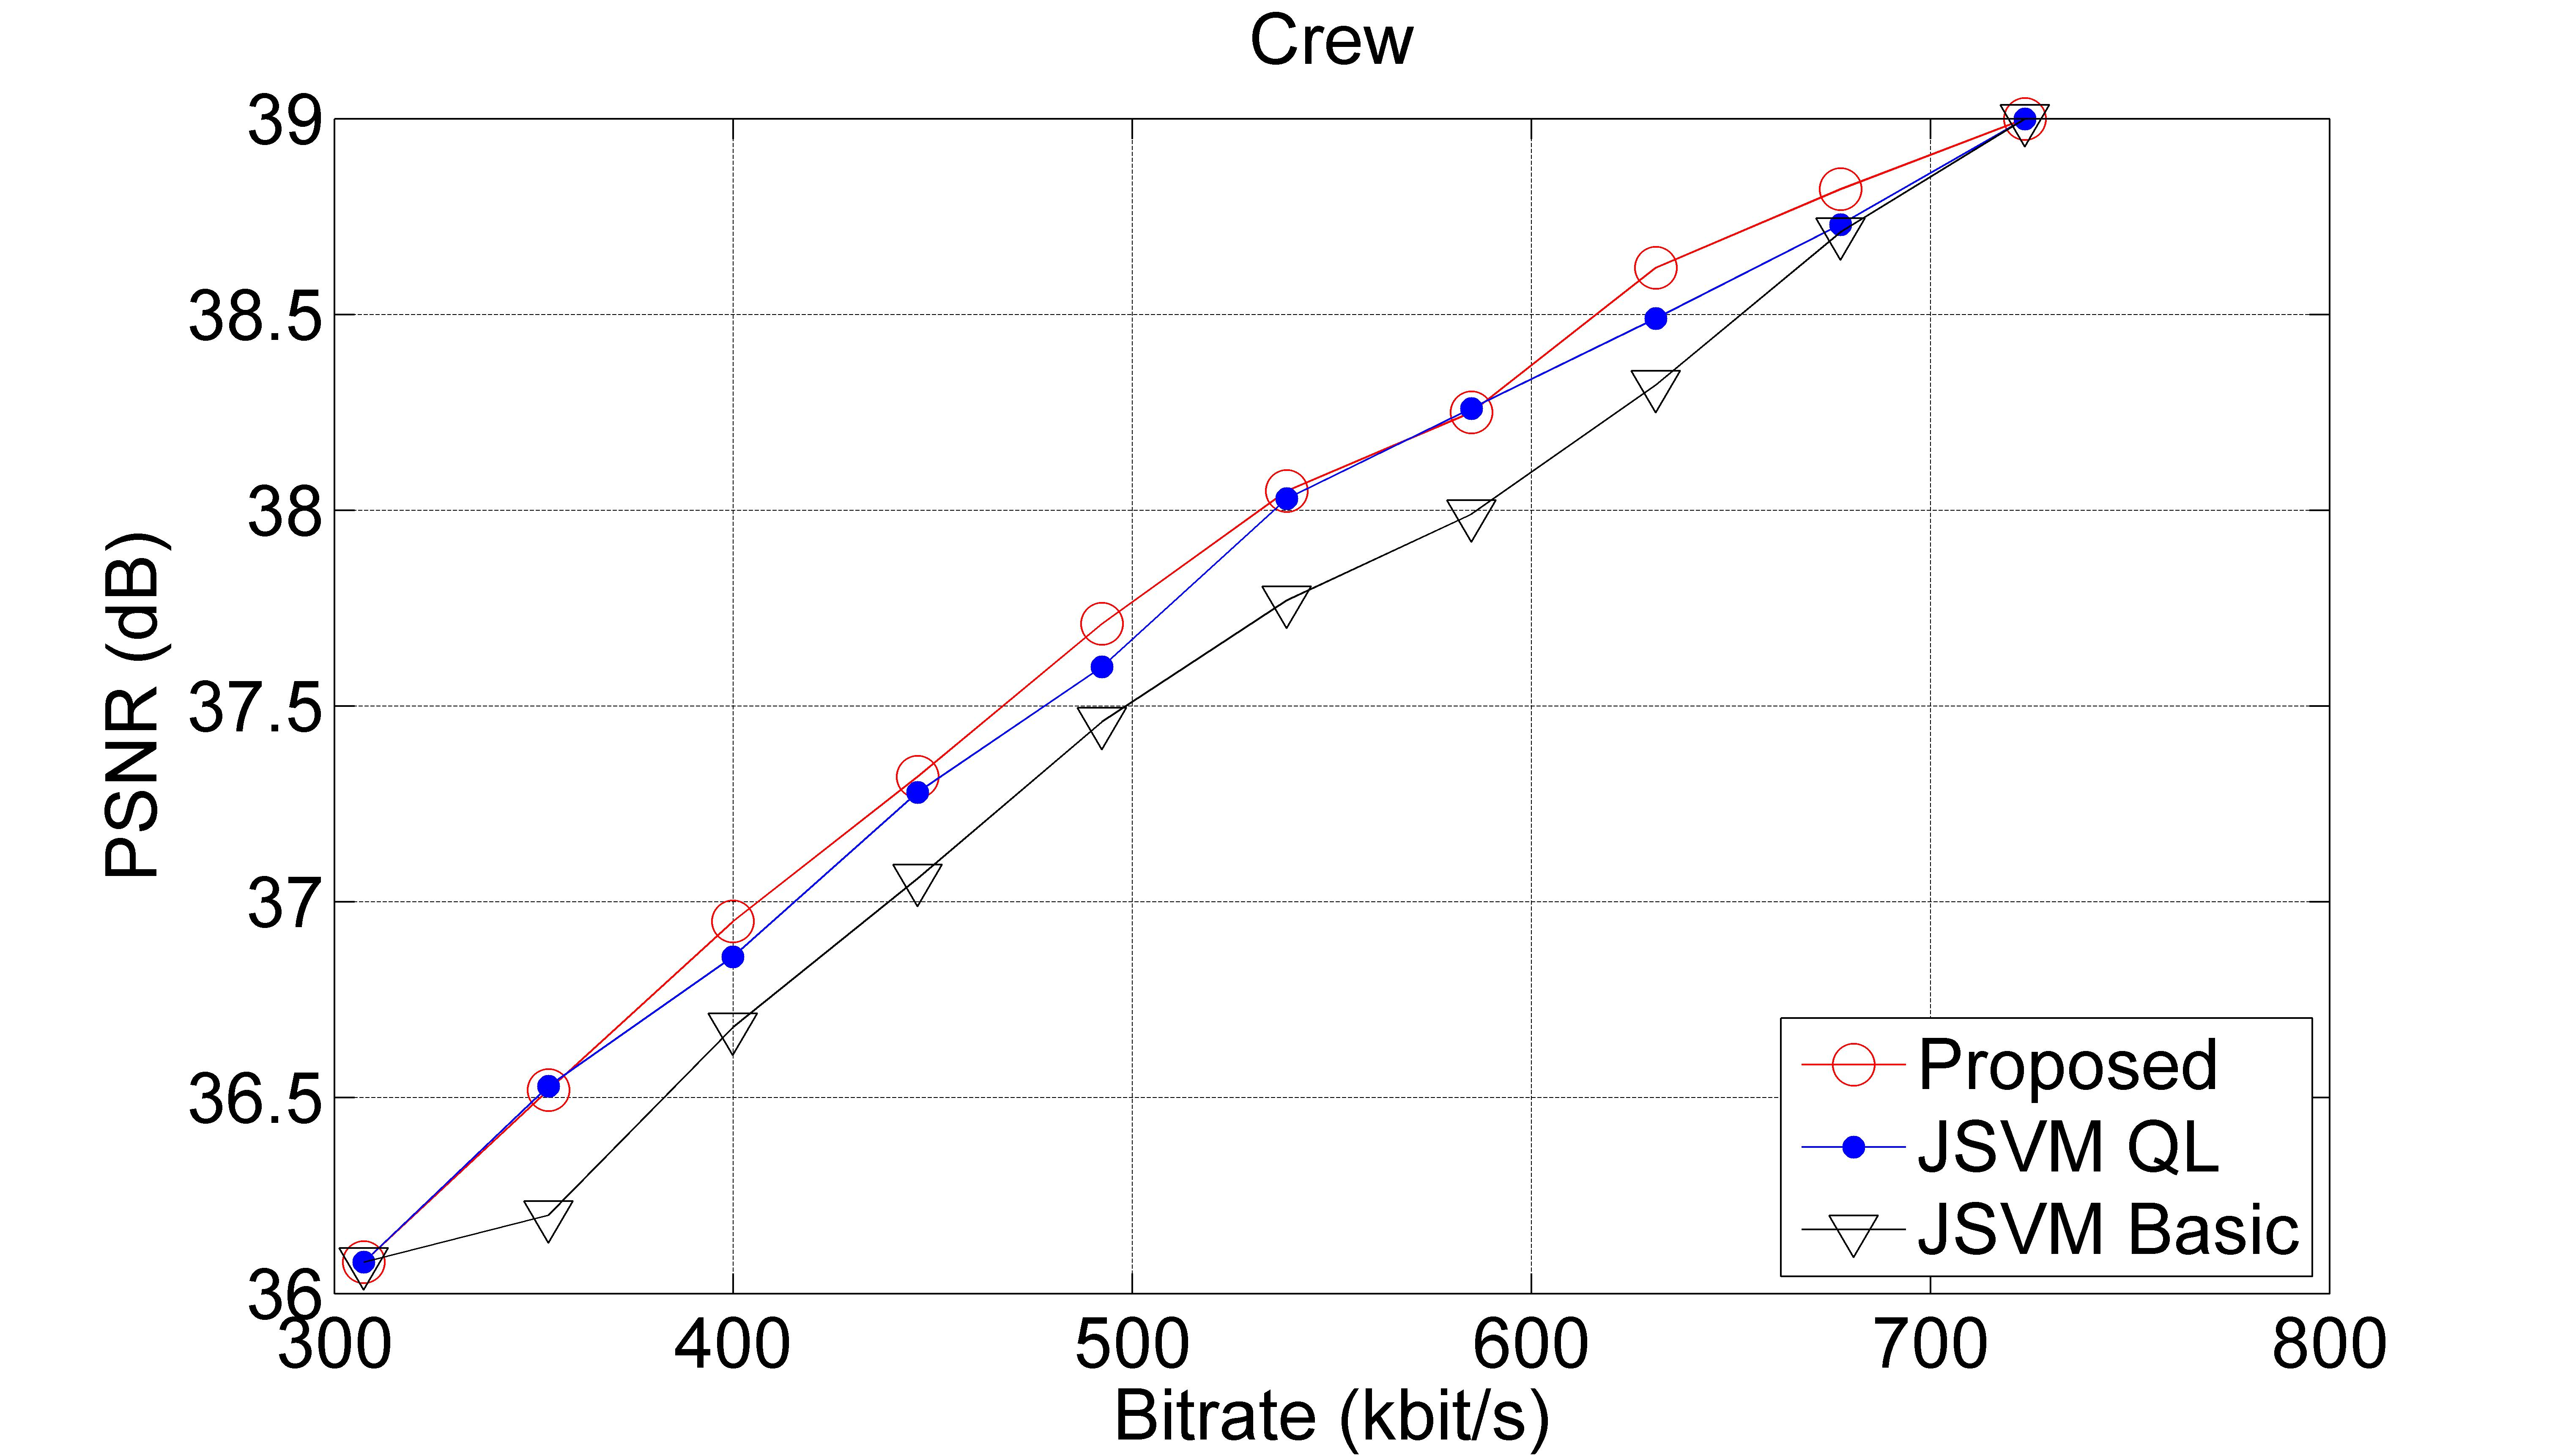
\includegraphics[width=0.5\textwidth]{figures/Crew.jpg}
		\label{fig:Crew}}
	\subfloat[Harbour]{
		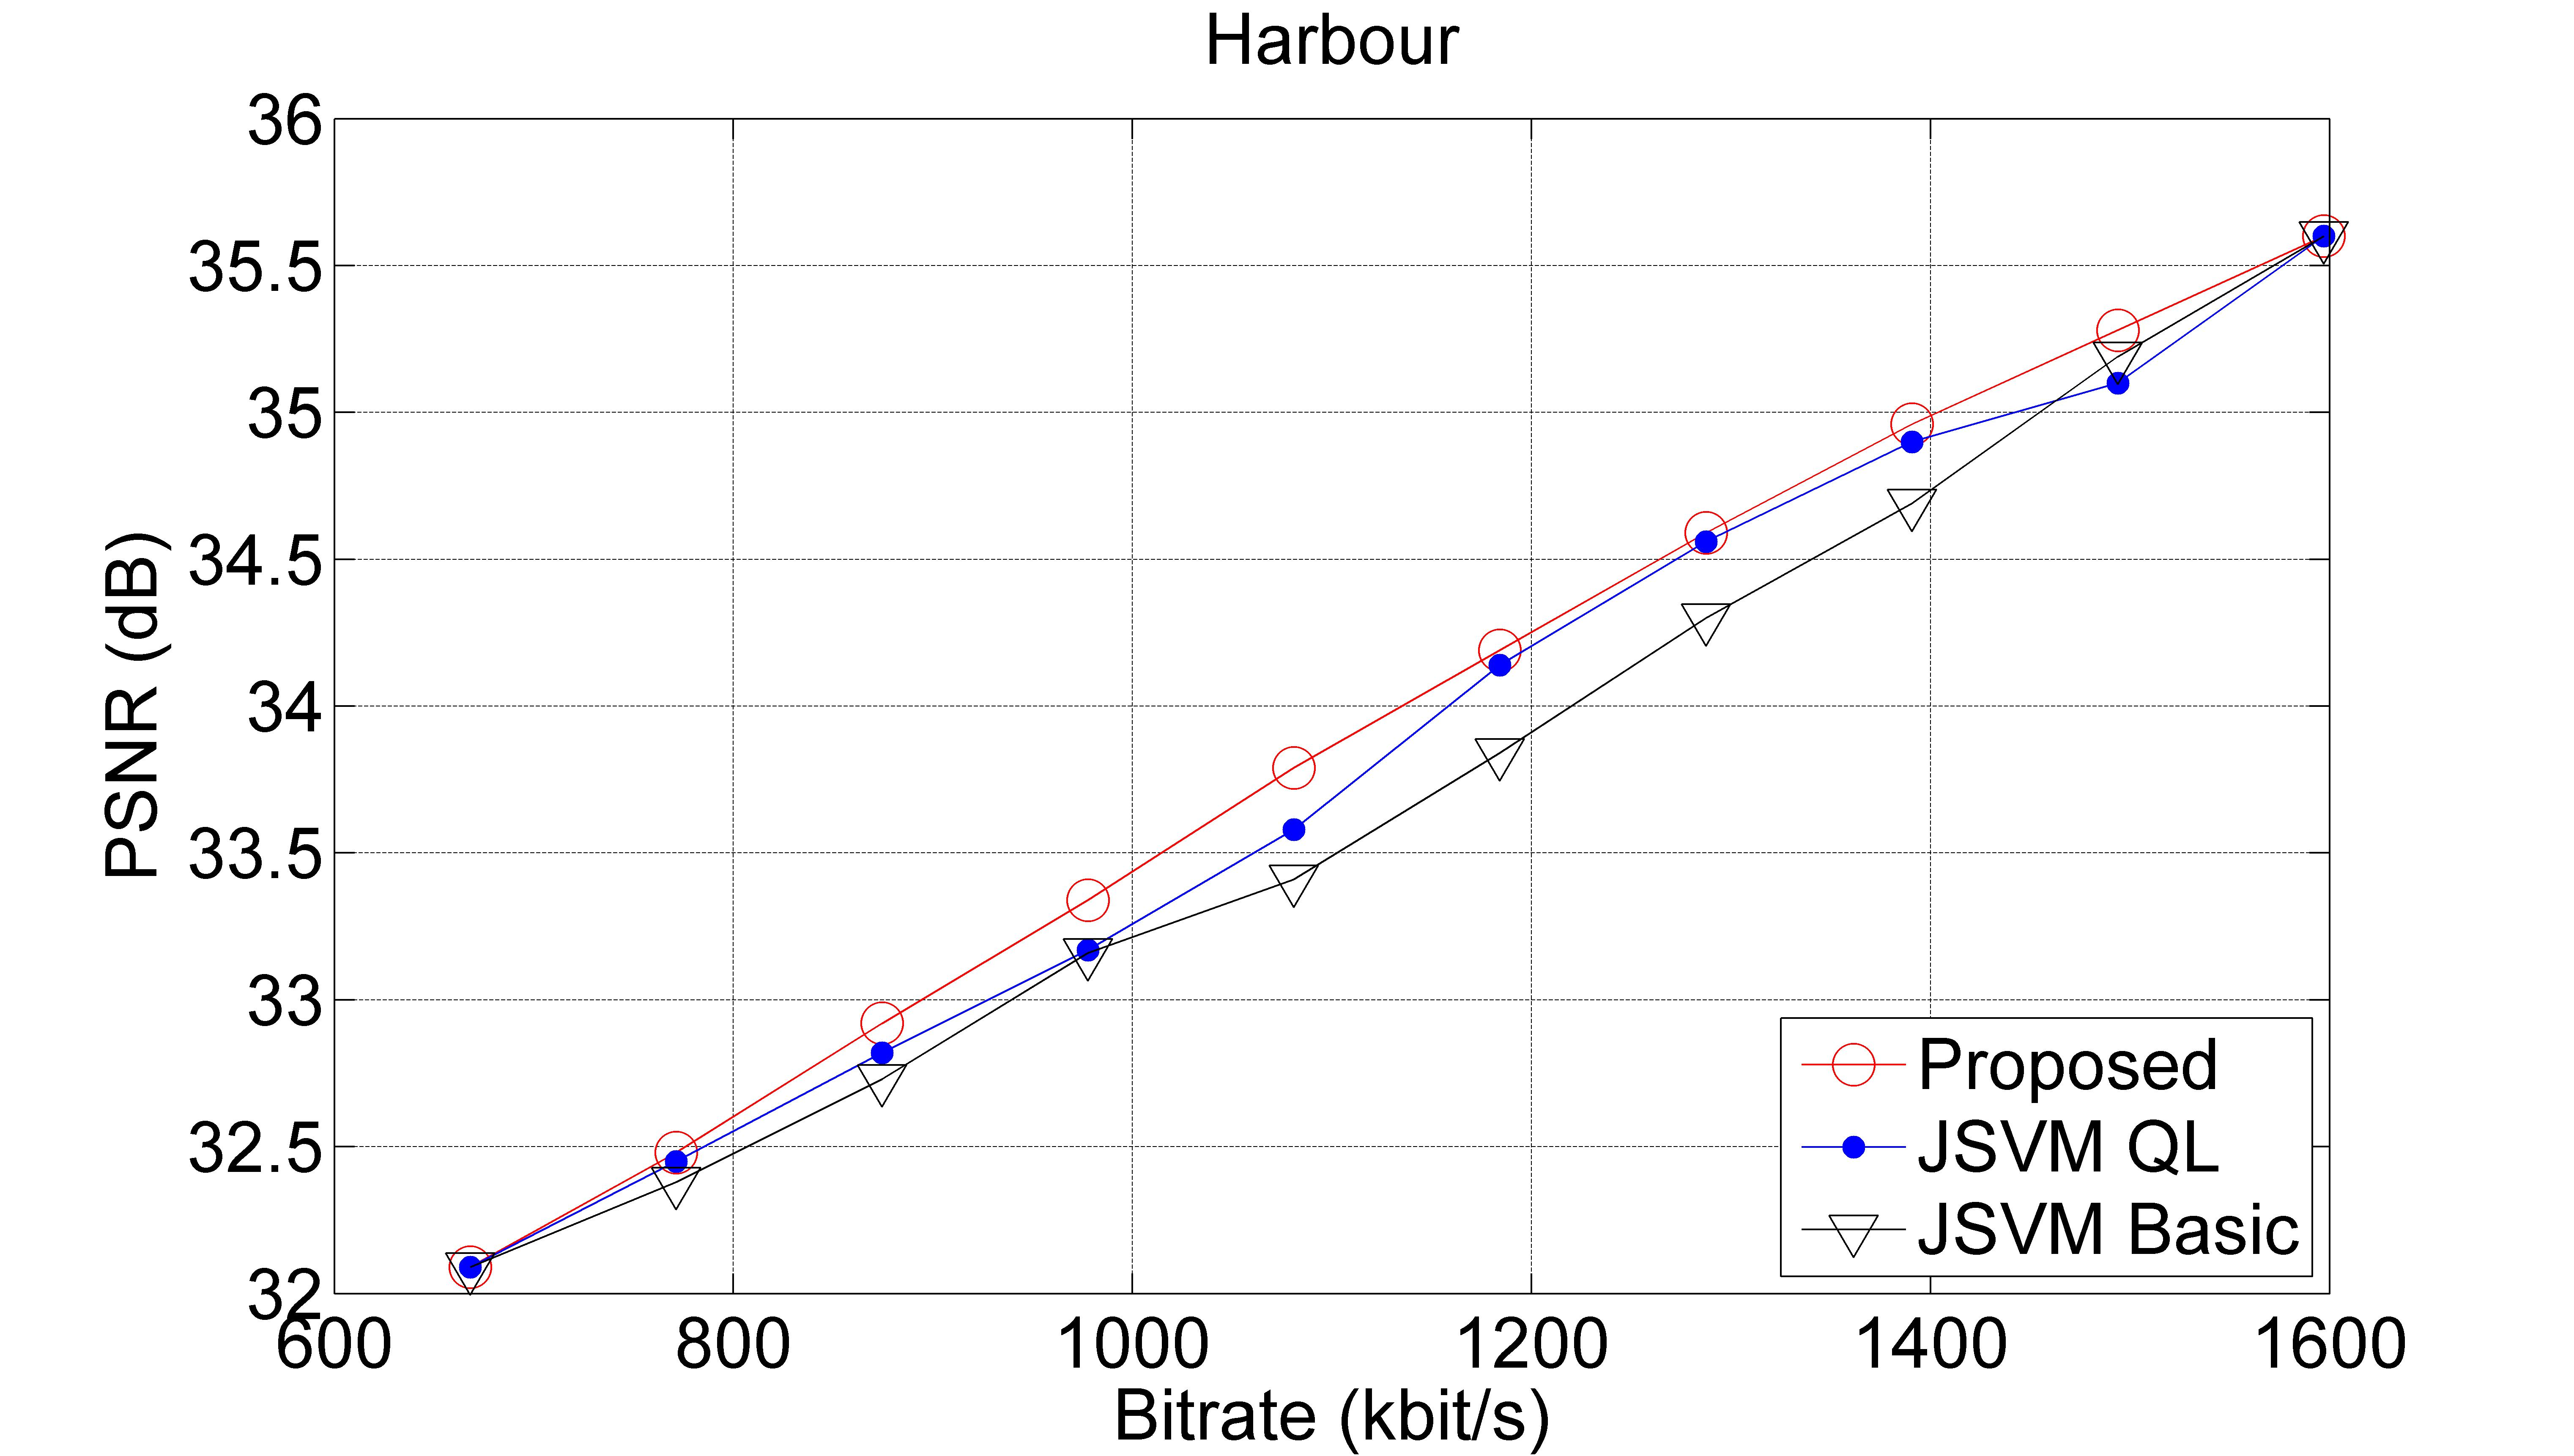
\includegraphics[width=0.5\textwidth]{figures/Harbour.jpg}
		\label{fig:Harbour}}
	\qquad
	\subfloat[Football]{
		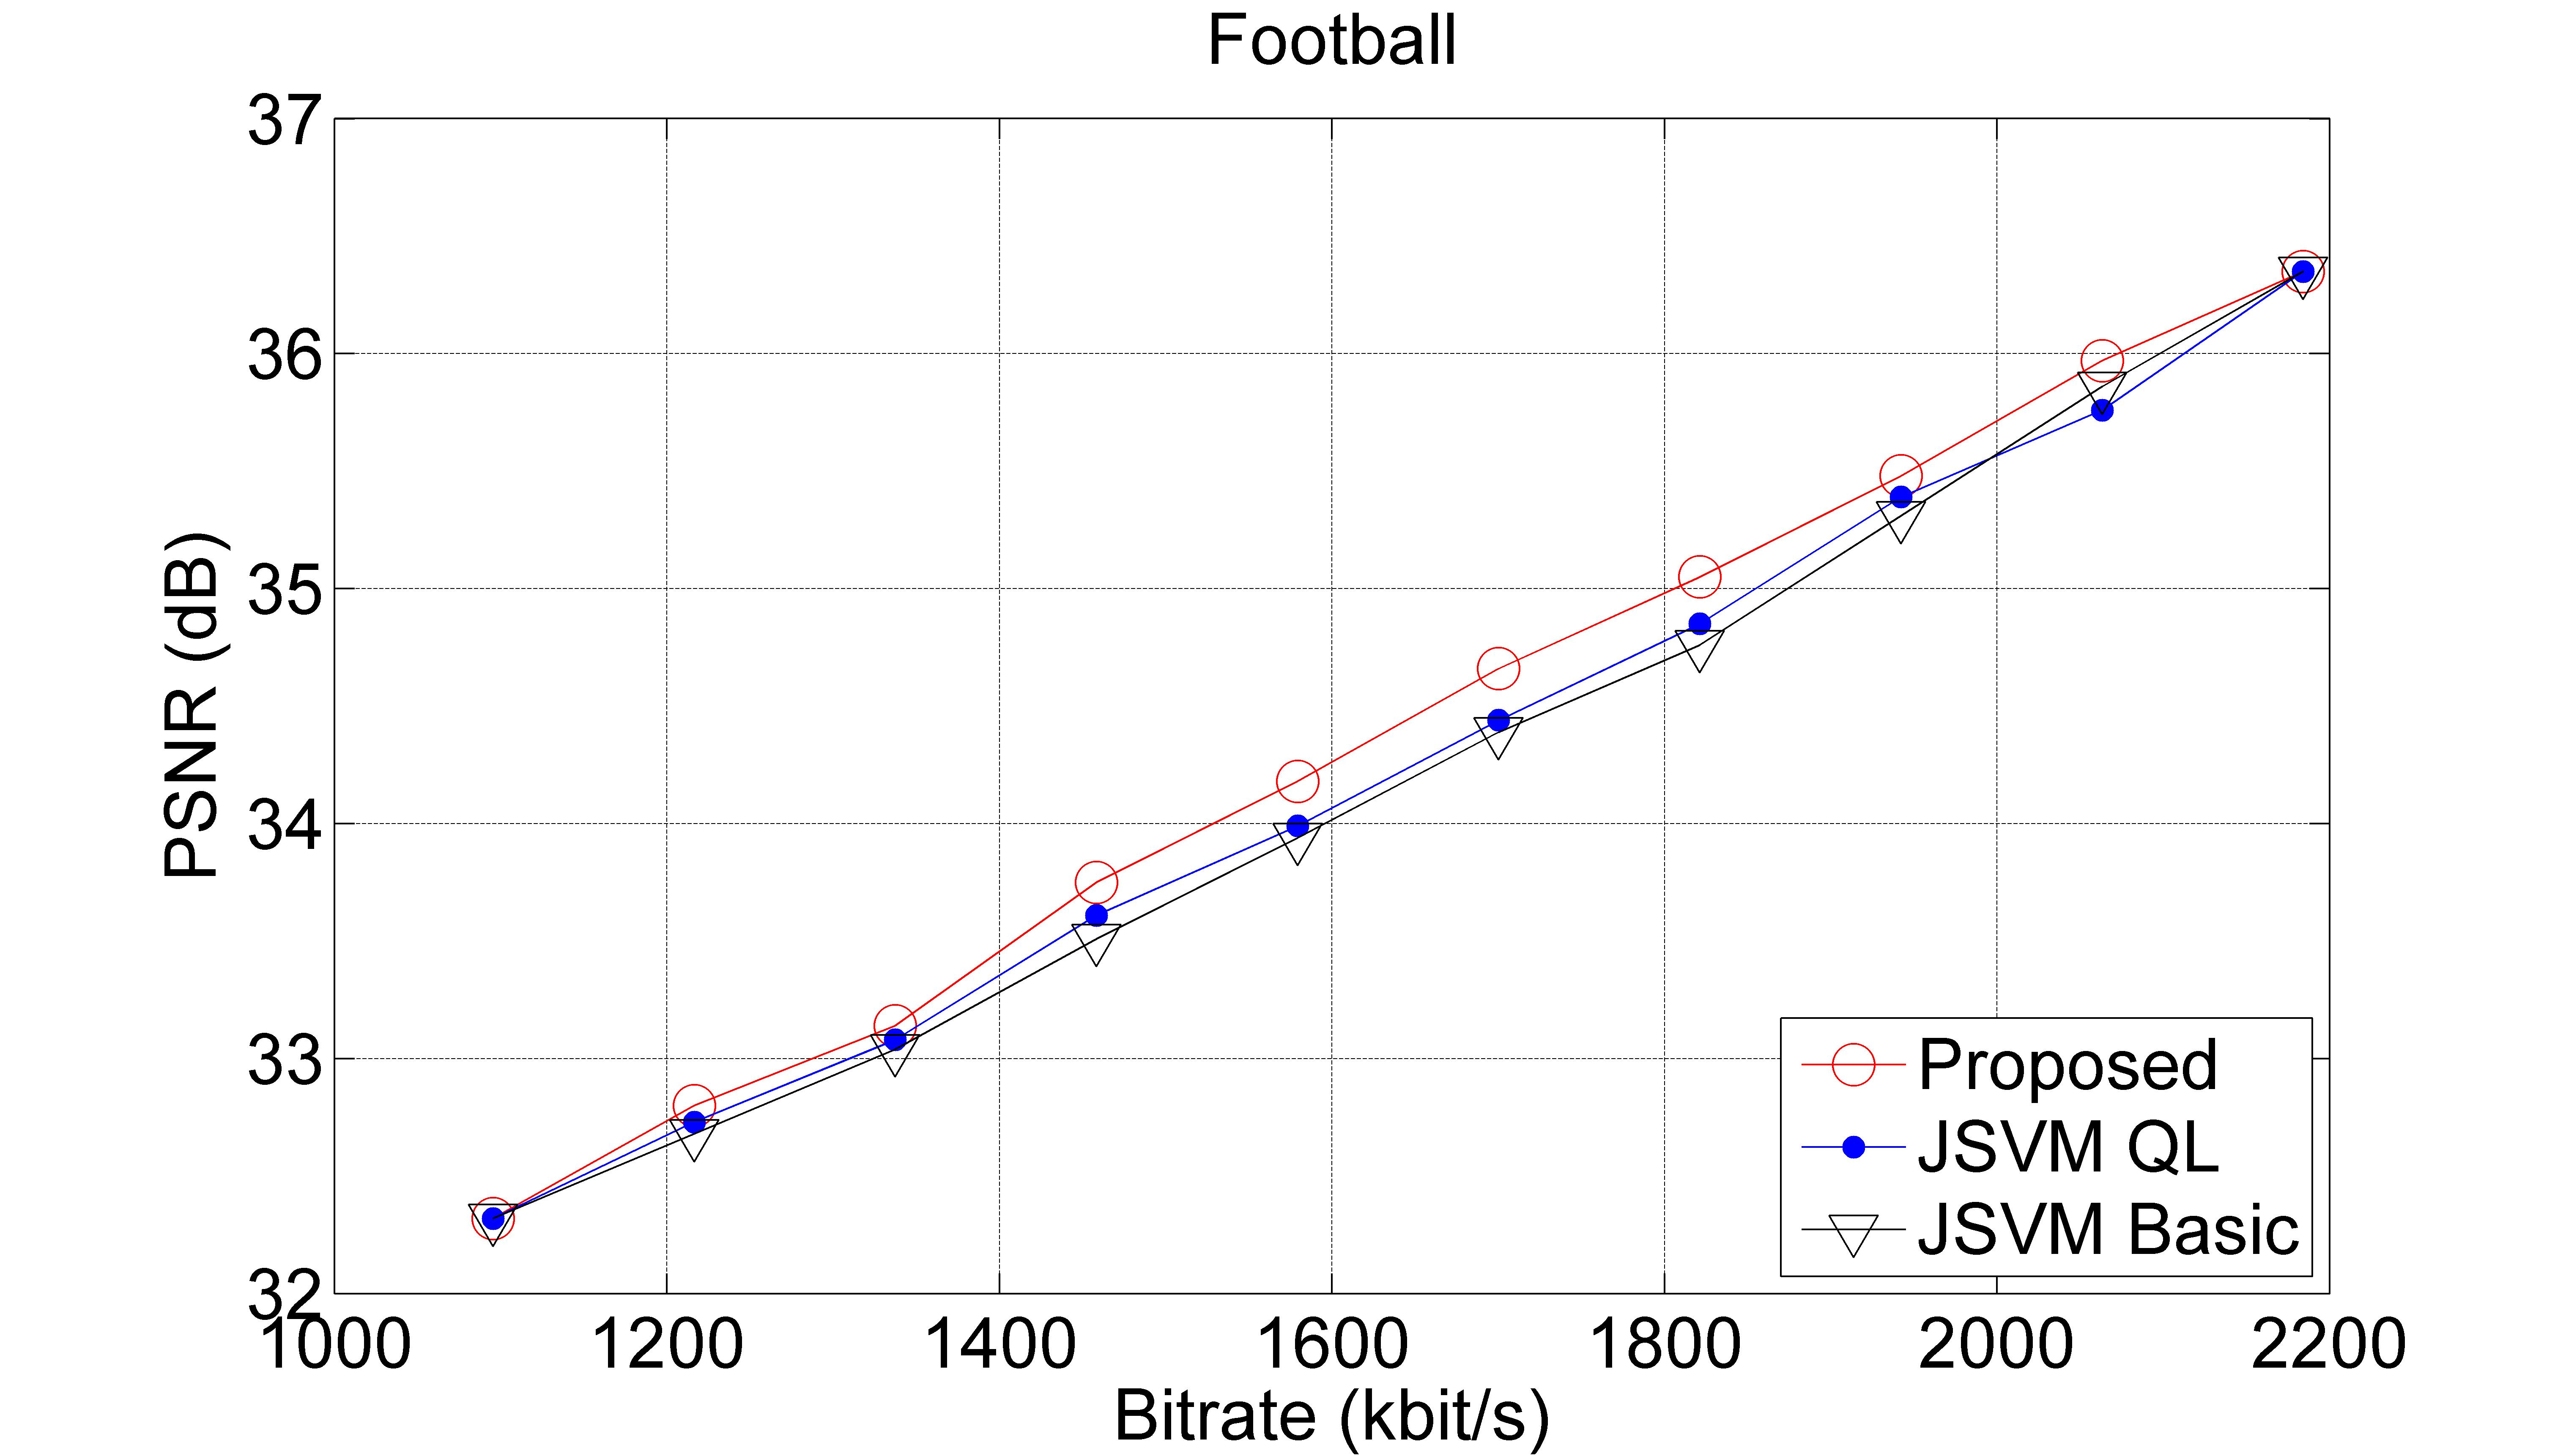
\includegraphics[width=0.5\textwidth]{figures/Football.jpg}
		\label{fig:Football}}
	\subfloat[Foreman]{
		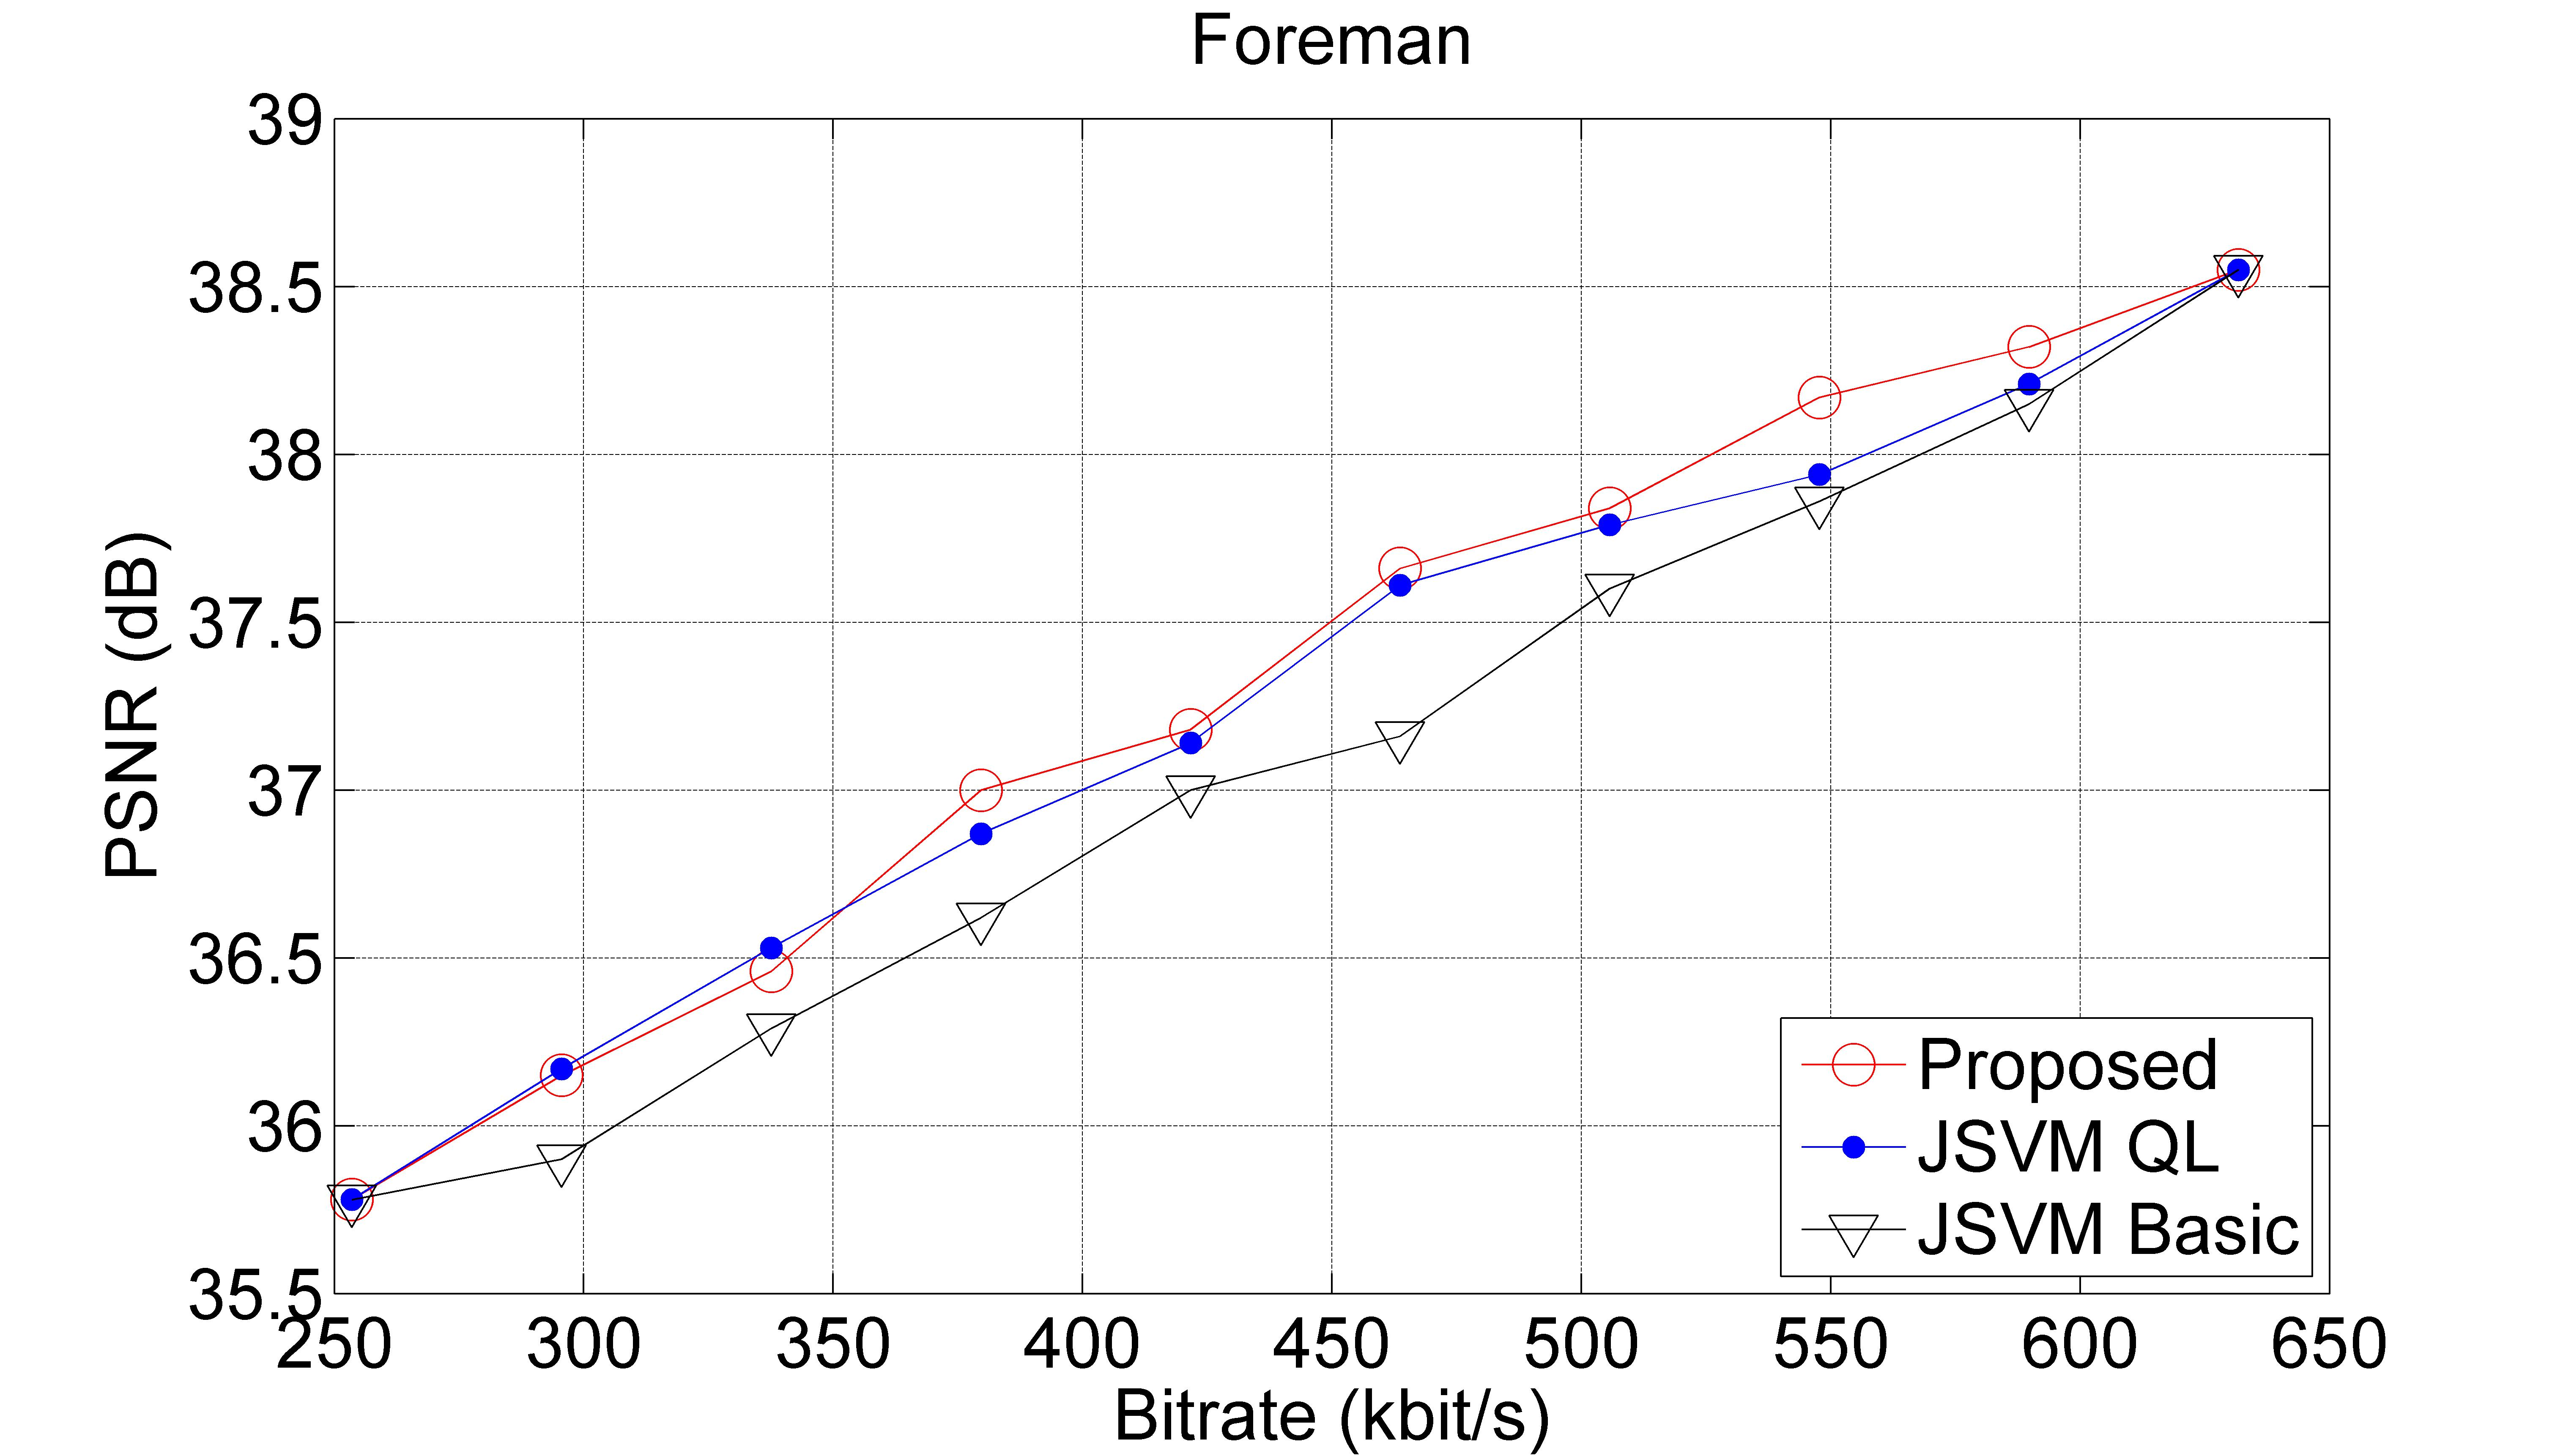
\includegraphics[width=0.5\textwidth]{figures/Foreman.jpg}
		\label{fig:Foreman}}
	\qquad
	\subfloat[Mobile]{
		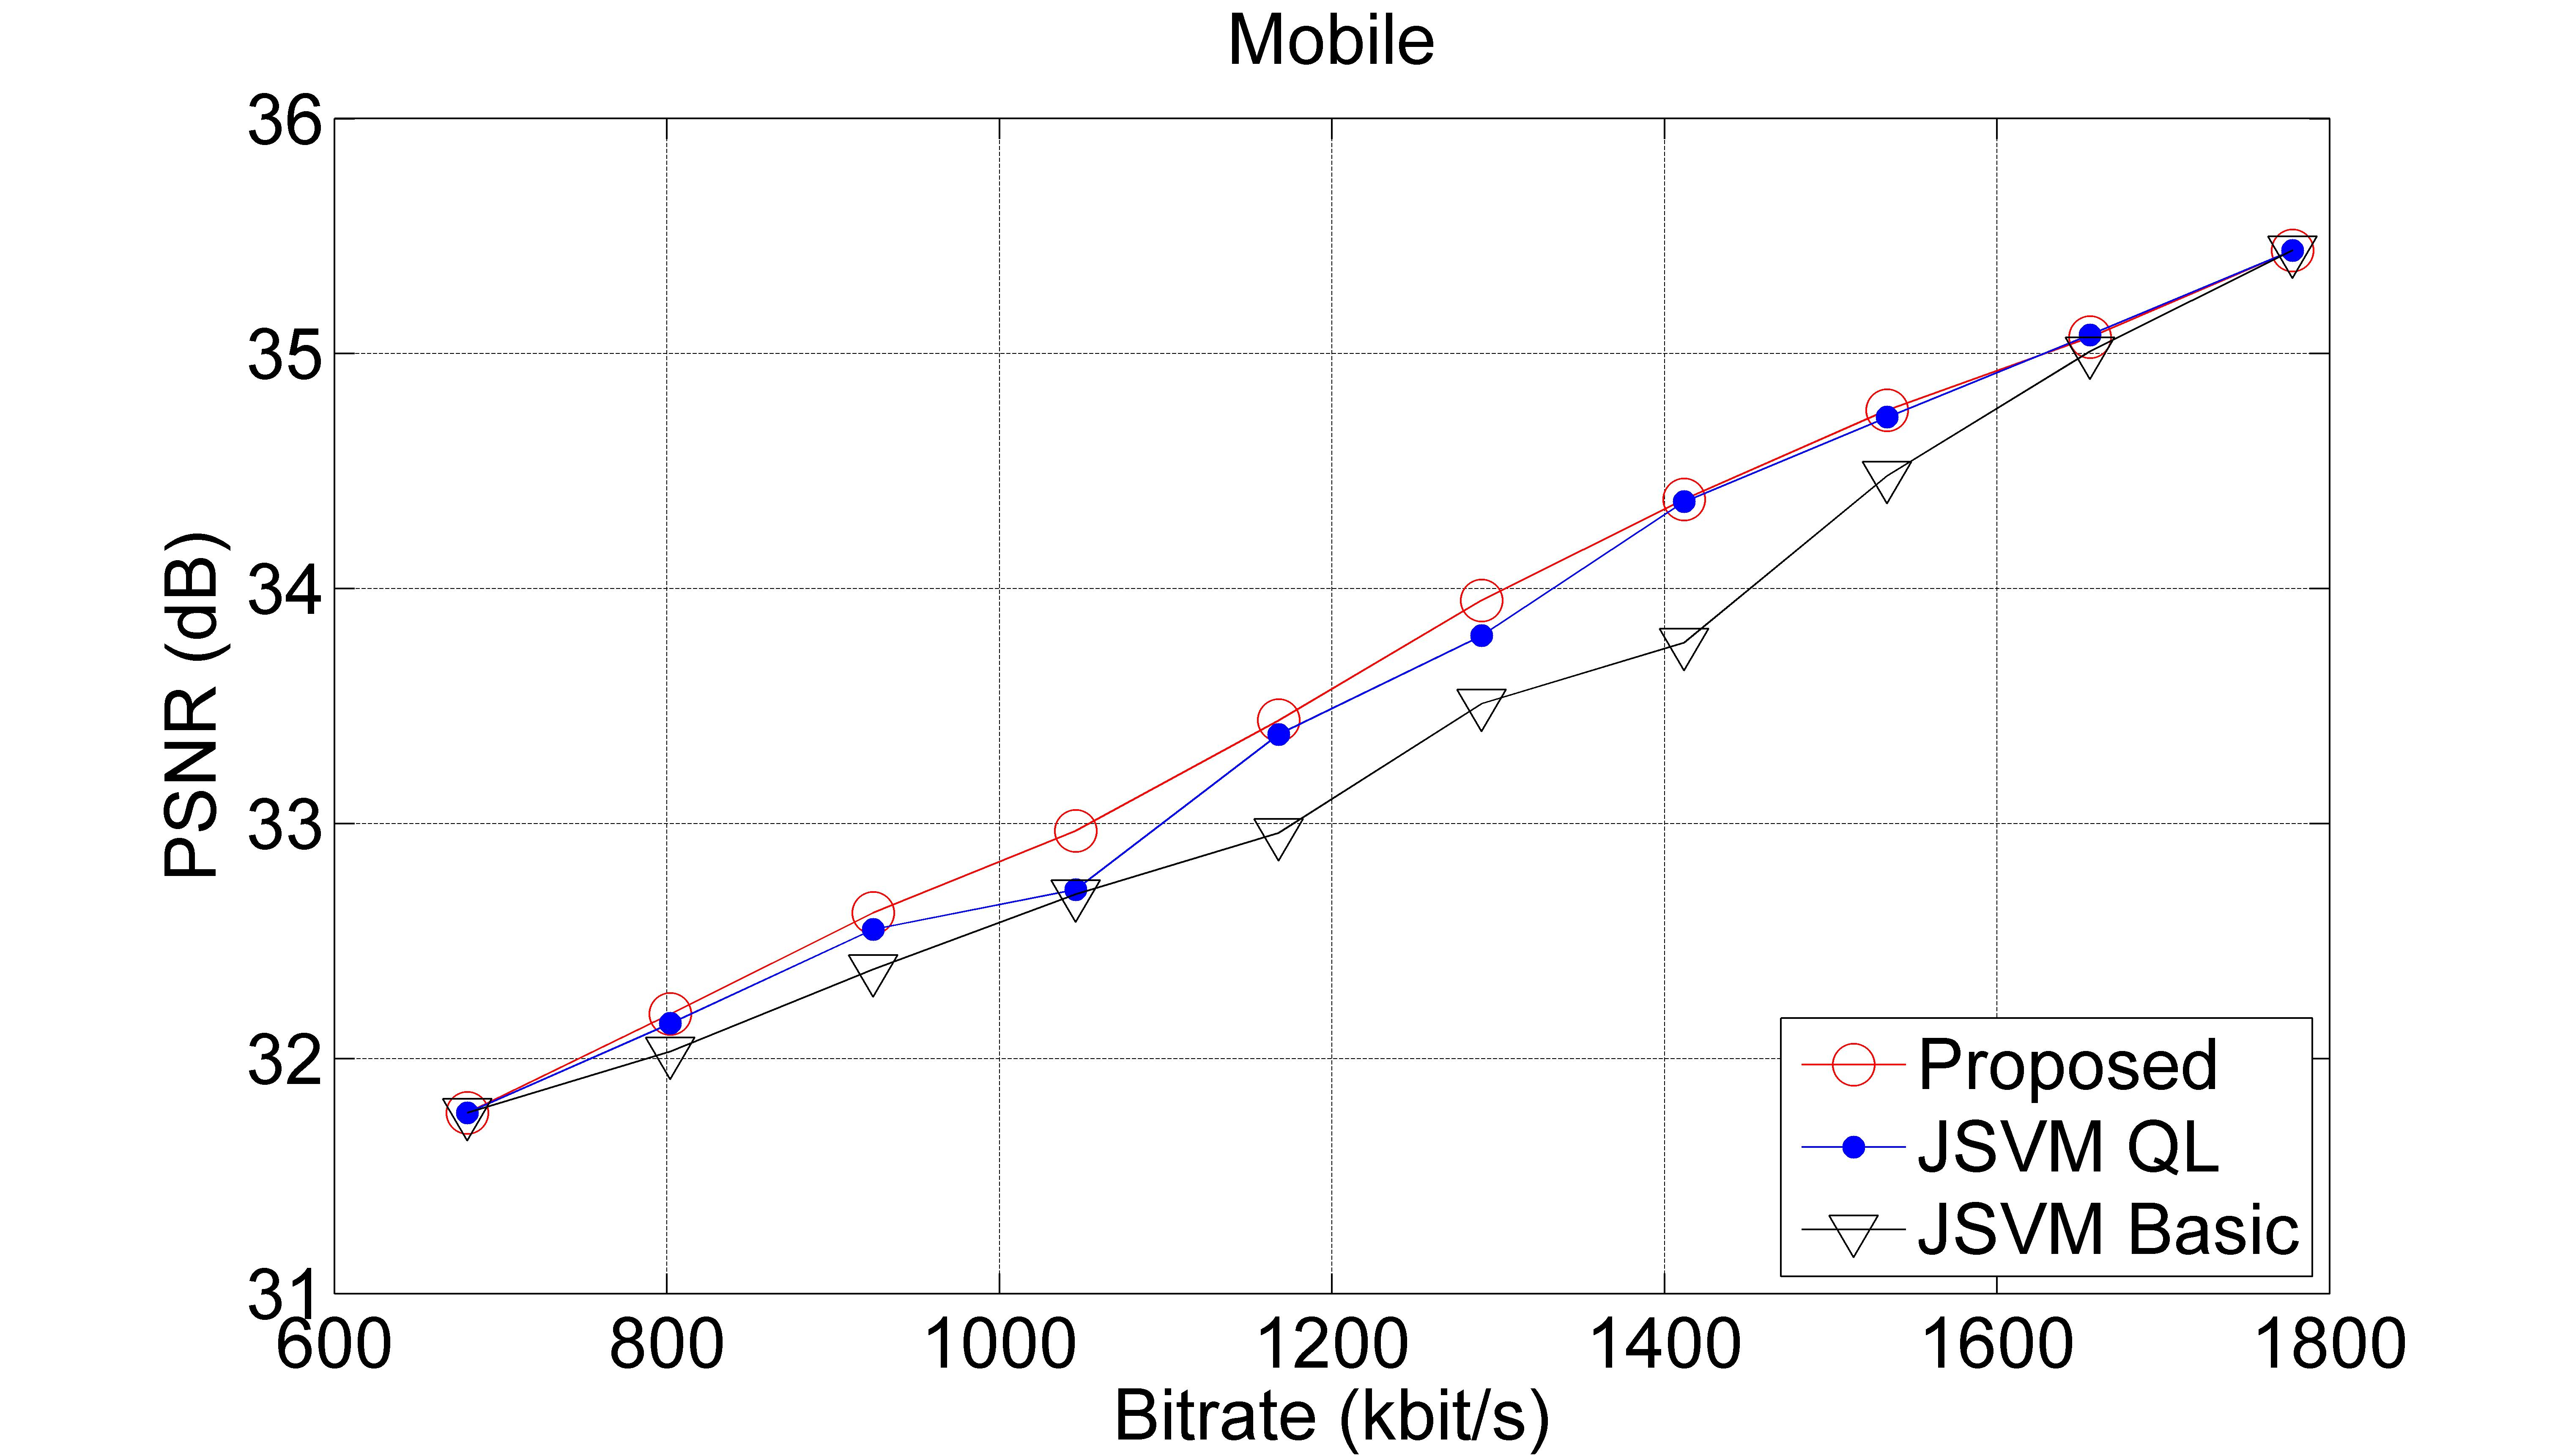
\includegraphics[width=0.5\textwidth]{figures/Mobile.jpg}
		\label{fig:Mobile}}
	\subfloat[Soccer]{
		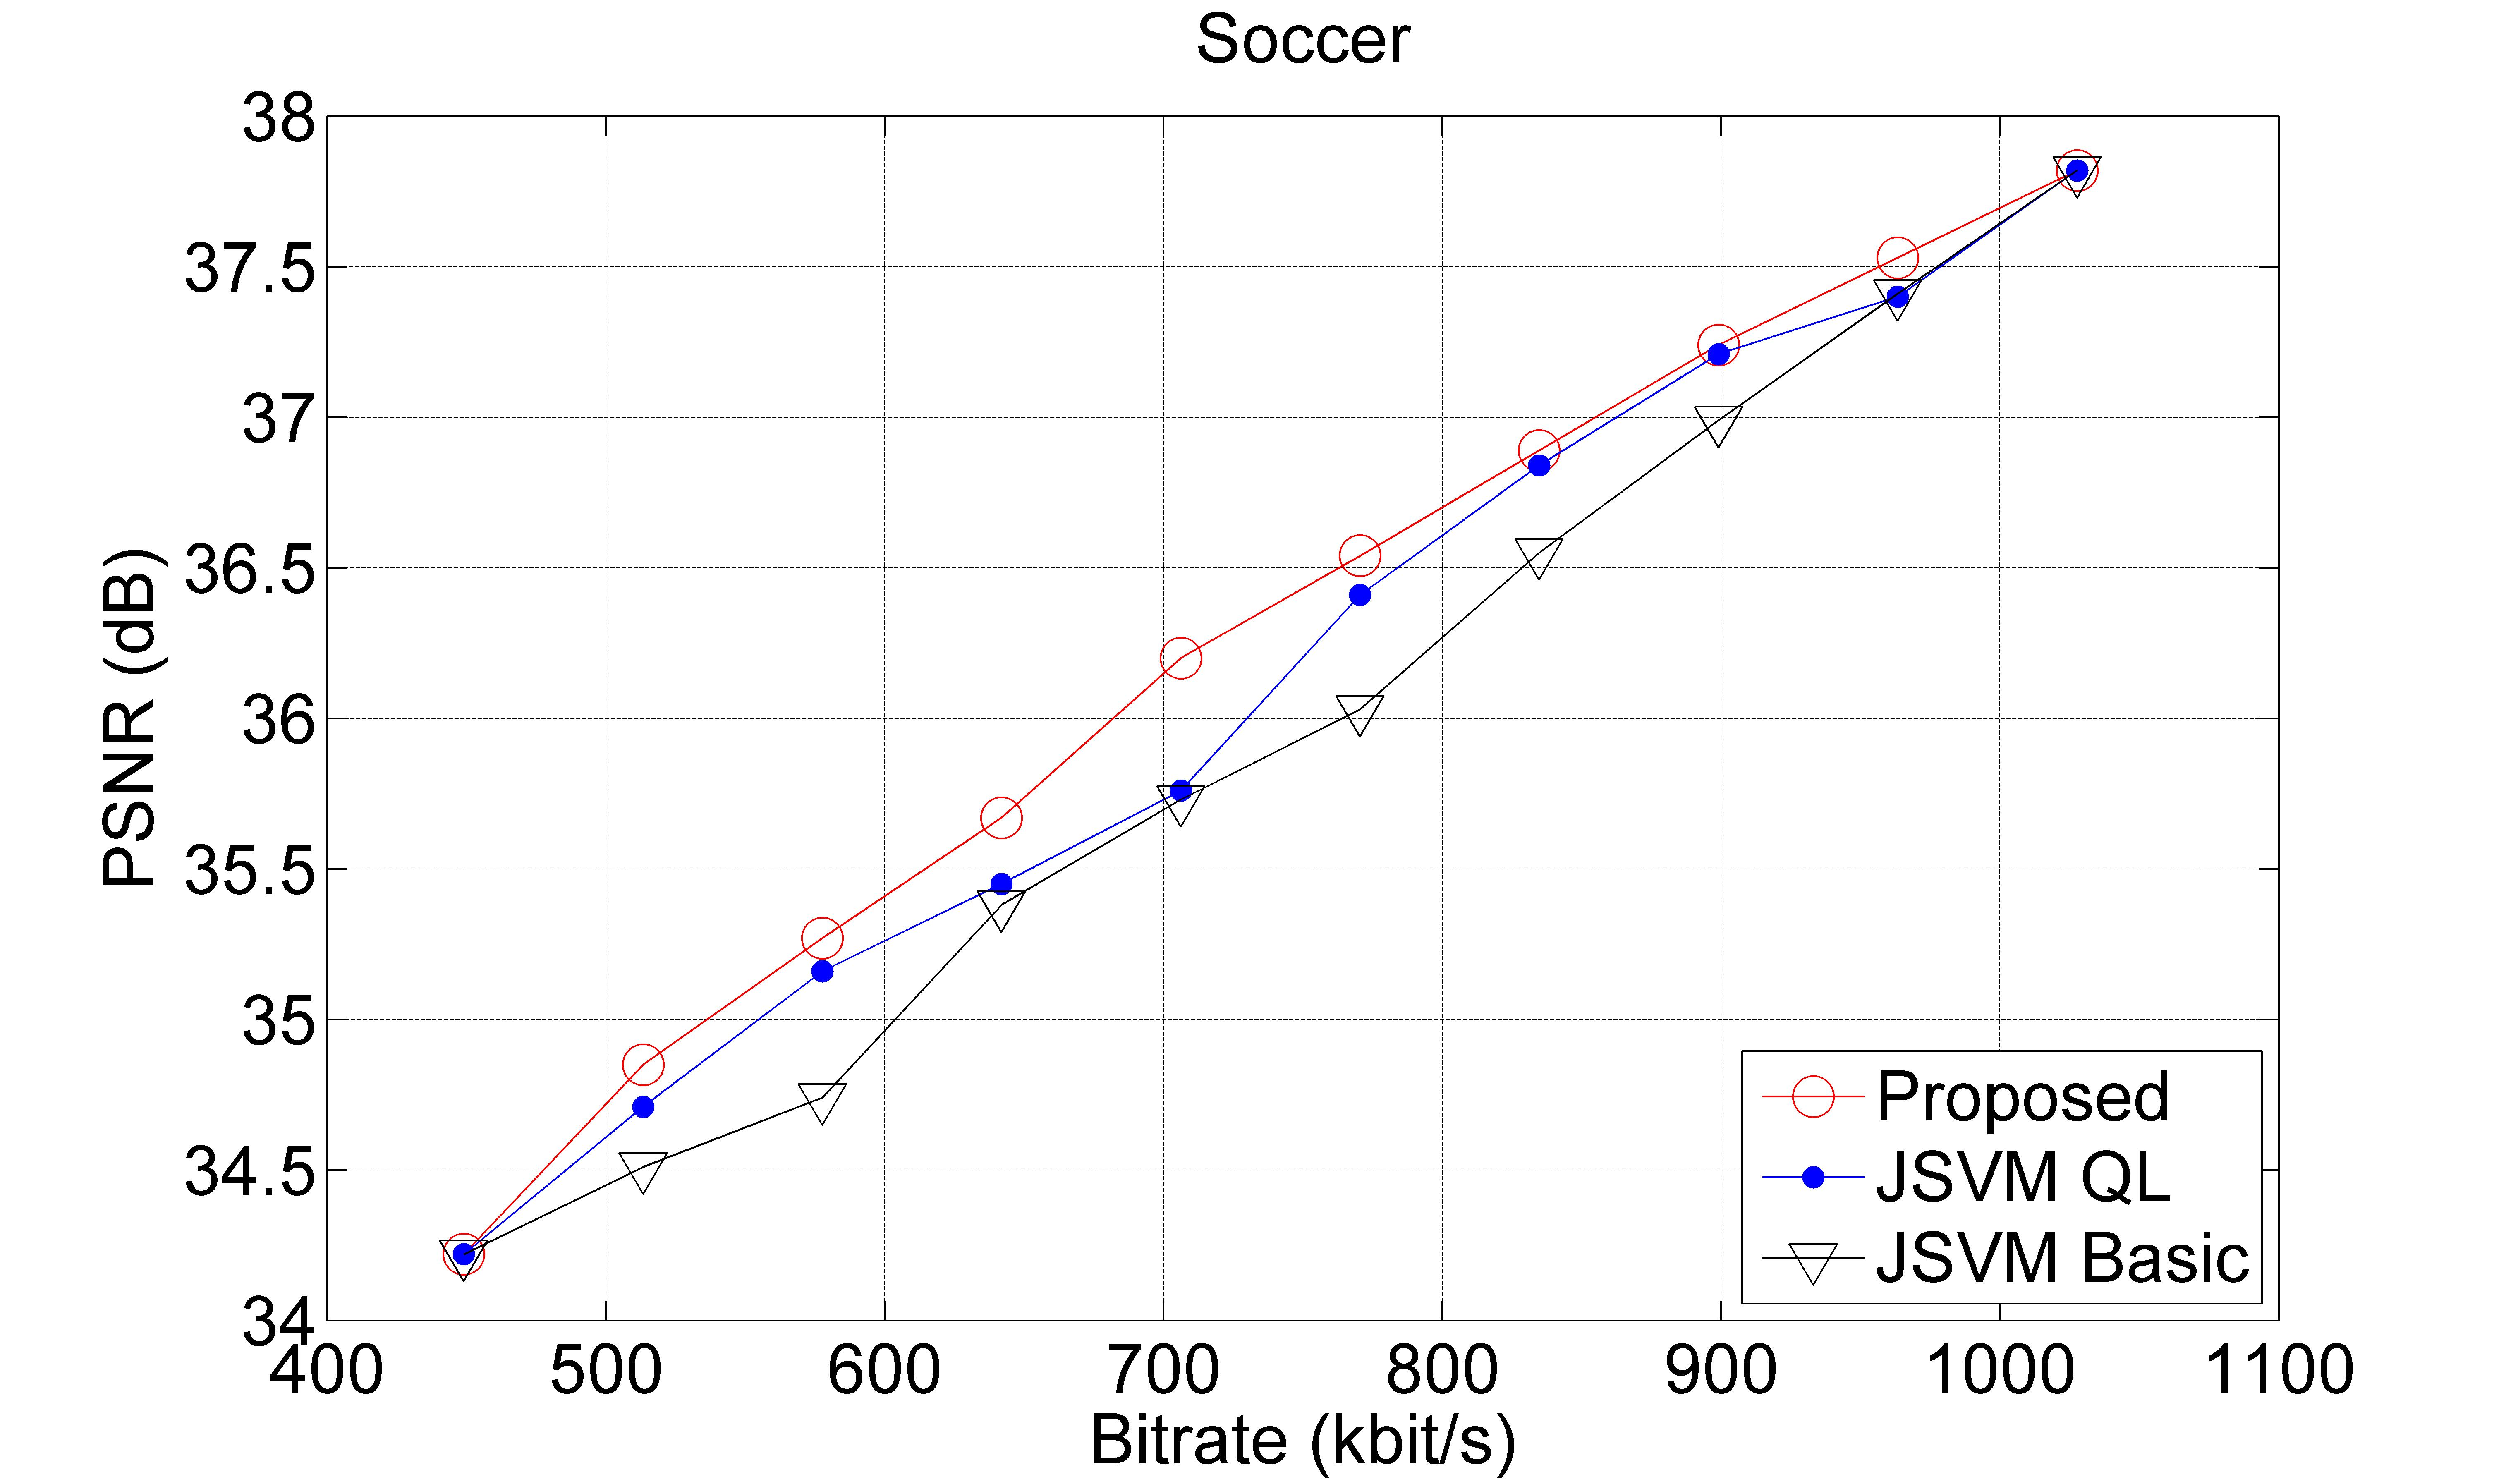
\includegraphics[width=0.5\textwidth]{figures/Soccer.jpg}
		\label{fig:Soccer}}
	\caption{三种码流截取方案的性能比较}
	\label{fig:extraction-performance}
\end{figure*}

图\ref{fig:extraction-performance}展示了全部八个测试序列的性能比较结果。可以看出,本文提出的方法对应的码率失真曲线几乎总是在最上方。这意味着在同样的码率限制下,本文提出的算法能取得更好的视频质量。注意到率失真曲线的第一个和最后一个点分别对应着最大程度截取和不进行截取的情况;在这两种情况下各种截取算法的结果是一样的,因此图中的三条曲线在这些点重合。

表\ref{tab:extraction-gain}列出了本文提出的截取方案相对于比较对象的PSNR提升。对于每一个测试序列,10个码率点的最大和平均PSNR提升都列了出来。可以看到,我们的方法相对于JSVM有明显的性能优势。该表中还列出了当优化窗口设置为48帧(也就是6个GOP)时的结果,证明了通过增大优化窗口确实能提升性能。不过在实际系统中,窗口大小还需考虑其他因素,并非能任意增大(参见\ref{subsec:priority-assign}小节末尾的分析)。

\begin{table*}[t]
	\centering
	\caption{本文提出的截取方案相比于JSVM的PSNR提升}
	\label{tab:extraction-gain}
	\small
	\begin{minipage}{1.0\linewidth}
		% \renewcommand{\thefootnote}{\thempfootnote}
		\centering
		\begin{tabular}{c|c|*{3}{p{0.9cm}<{\centering}|}*{4}{p{1.1cm}<{\centering}|}p{0.9cm}<{\centering}}
			%% |l|l| to left justify each column entry
			%% |c|c| to center each column entry
			%% use of \rule[]{}{} below opens up each row
			\hline \hline
			\multicolumn{2}{c|}{序列名} &
			{\em Bus} & {\em City} & {\em Crew} & {\em Football} & {\em Foreman} & {\em Harbour} & {\em Mobile} & {\em Soccer} \\ \hline 
			\multirow{2}{*}{JSVM QL, $K$ = 32 \footnote{\label{footnote:JSVM_QL} 与JSVM QL对比;优化窗口大小为32帧}}
			& Max\footnote{\label{footnote:max} 所有码率限制下的最大提升}
			& 0.37 & 0.50 & 0.13 & 0.22 & 0.23 & 0.19 & 0.25 & 0.44 \\ \cline{2-10}
			& Ave\footnote{\label{footnote:ave} 所有码率限制下的平均提升}
			& 0.11 & 0.11 & 0.05 & 0.12 & 0.05 & 0.05 & 0.06 & 0.13 \\ \hline
			\multirow{2}{*}{JSVM Basic, $K$ = 32}
			& Max & 0.50 & 0.83 & 0.32 & 0.29 & 0.50 & 0.34 & 0.61 & 0.53 \\ \cline{2-10}
			& Ave & 0.18 & 0.37 & 0.20 & 0.15 & 0.22 & 0.15 & 0.25 & 0.29 \\ \Xhline{2\arrayrulewidth}
			\multirow{2}{*}{JSVM QL, $K$ = 48}
			& Max & 0.36 & 0.39 & 0.27 & 0.30 & 0.30 & 0.38 & 0.21 & 0.40 \\ \cline{2-10}
			& Ave & 0.12 & 0.23 & 0.16 & 0.13 & 0.15 & 0.13 & 0.08 & 0.21 \\ \hline
			\multirow{2}{*}{JSVM Basic, $K$ = 48}
			& Max & 0.36 & 0.81 & 0.32 & 0.29 & 0.49 & 0.47 & 0.57 & 0.60 \\ \cline{2-10}
			& Ave & 0.19 & 0.40 & 0.19 & 0.17 & 0.28 & 0.22 & 0.28 & 0.42 \\ \hline
		\end{tabular}
	\end{minipage}
\end{table*}

最后需要指出,在JSVM之外的其他码流截取方法中,Maani等人的工作\supercite{Maani2009}取得了比JSVM QL高得多的性能,甚至比本文提出的方法性能还好。但是,为了得到适用于不同序列的鲁棒的模型参数,该工作中的方法需要更多的计算量去训练。而本文提出的方法所需计算量总是与JSVM相当的。据我们所知,在不显著增加计算量的情况下,码流截取很难取得较大的PSNR提升。

\subsection{无参考截取实验}

\begin{figure*}[!ht]
	\centering
	\subfloat[Bus]{
		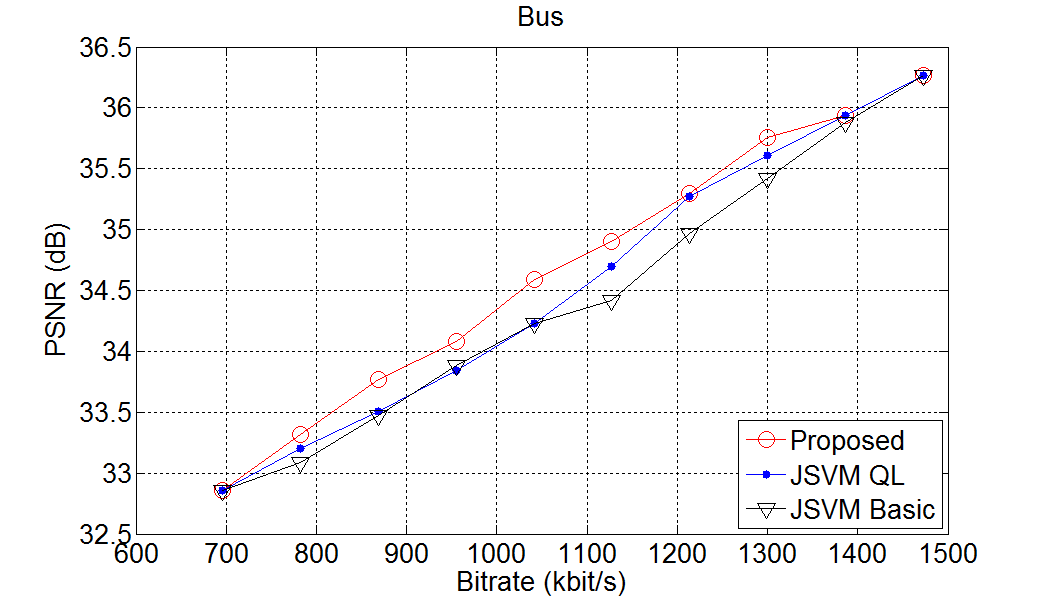
\includegraphics[width=0.5\textwidth]{figures/Bus-noref.png}}
	\subfloat[City]{
		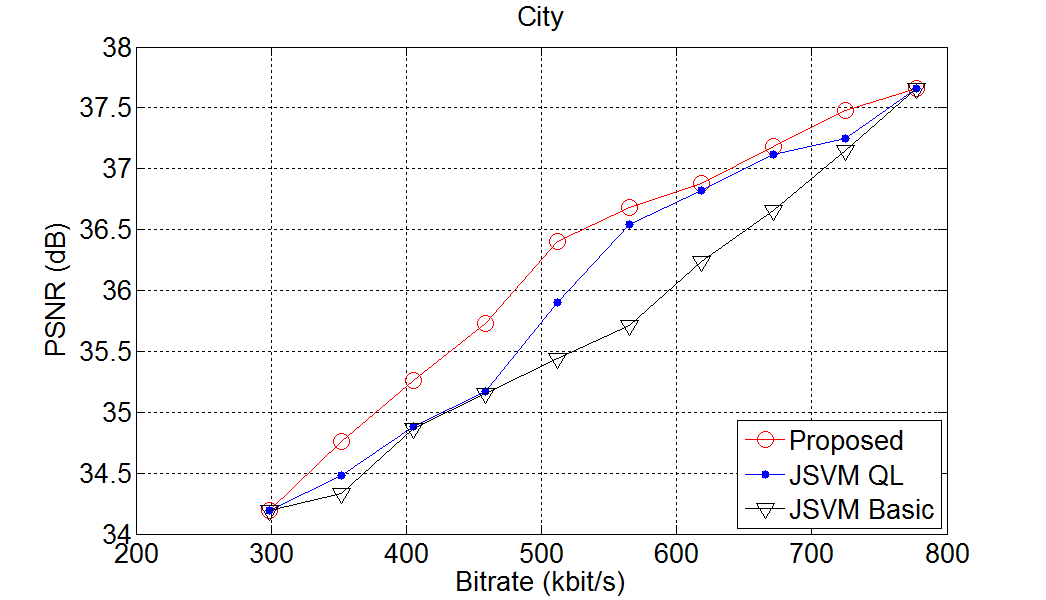
\includegraphics[width=0.5\textwidth]{figures/City-noref.png}}
	\qquad
	\subfloat[Crew]{
		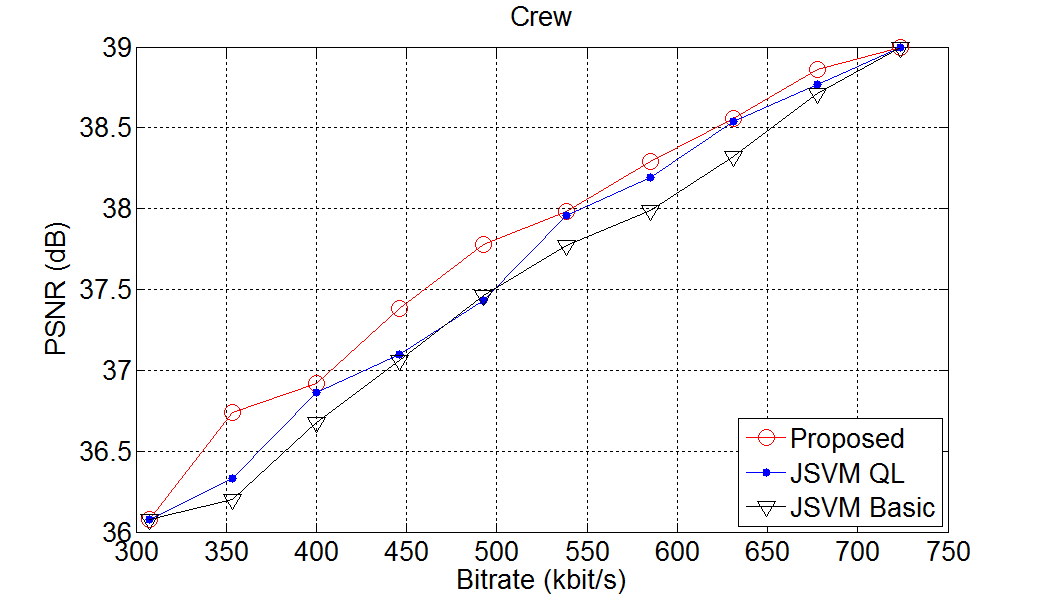
\includegraphics[width=0.5\textwidth]{figures/Crew-noref.png}}
	\subfloat[Harbour]{
		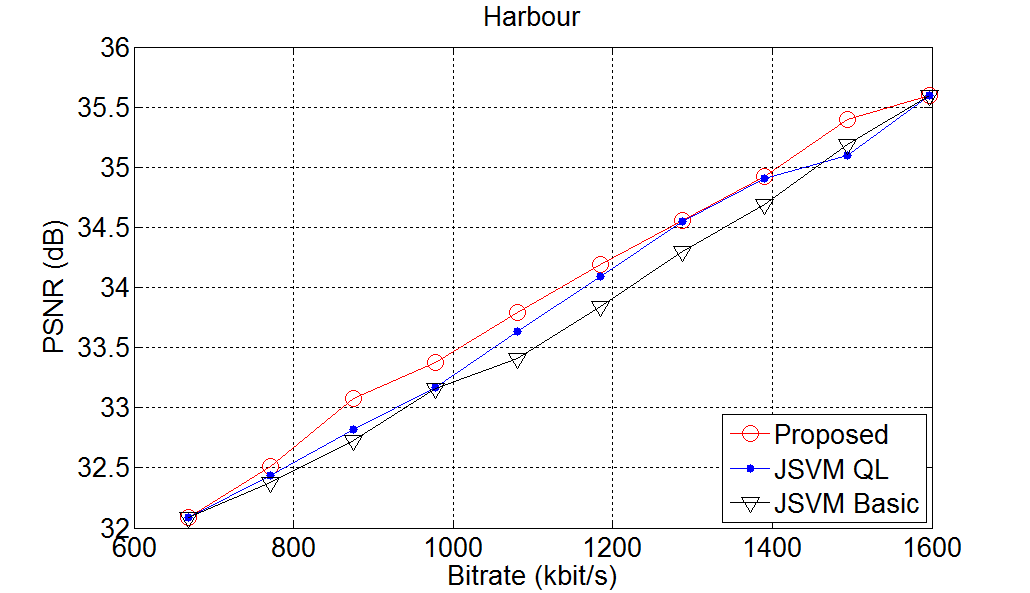
\includegraphics[width=0.5\textwidth]{figures/Harbour-noref.png}}
	\qquad
	\subfloat[Football]{
		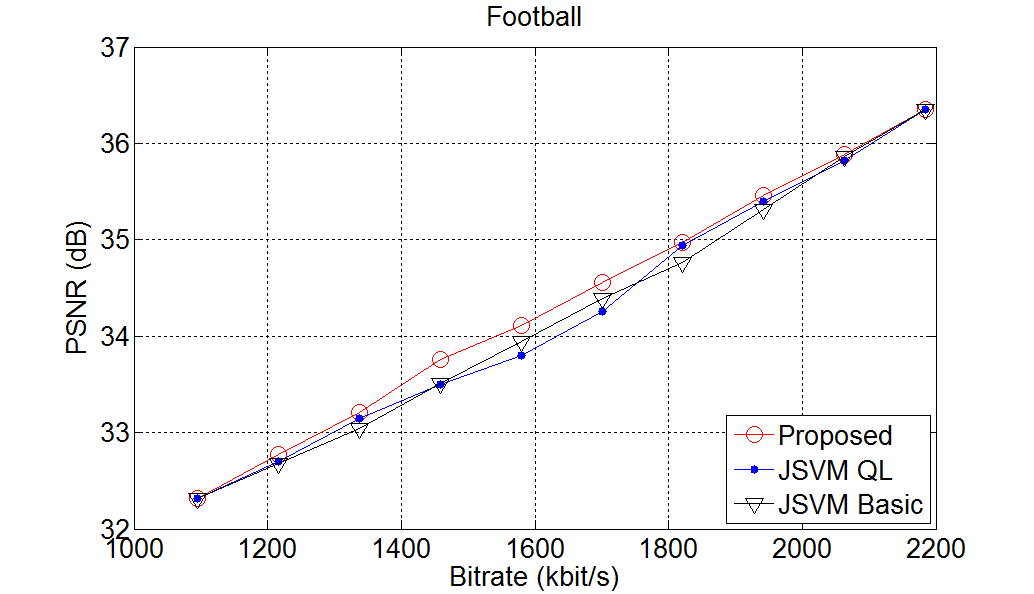
\includegraphics[width=0.5\textwidth]{figures/Football-noref.png}}
	\subfloat[Foreman]{
		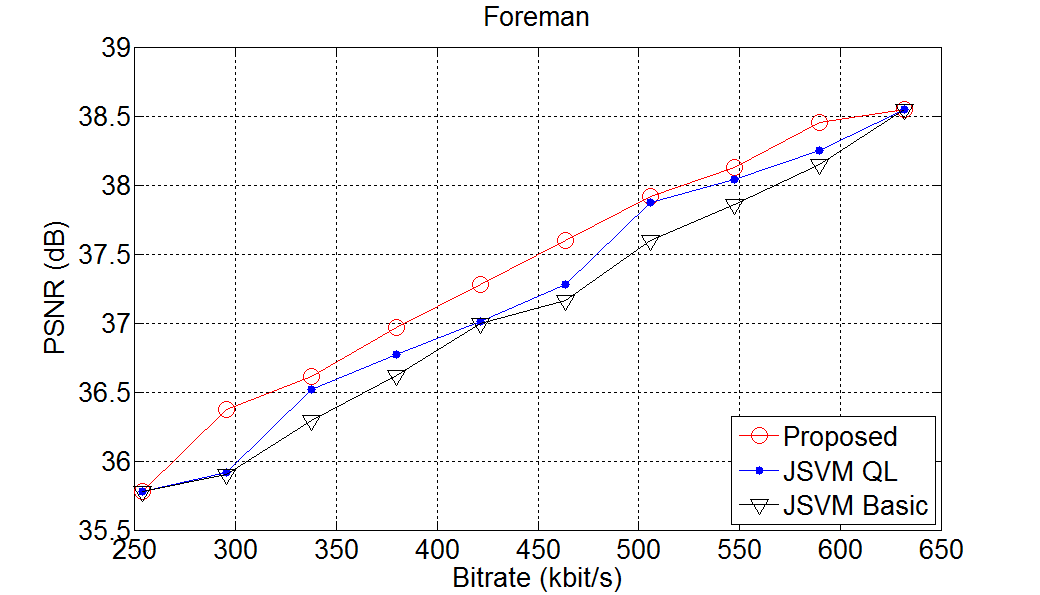
\includegraphics[width=0.5\textwidth]{figures/Foreman-noref.png}}
	\qquad
	\subfloat[Mobile]{
		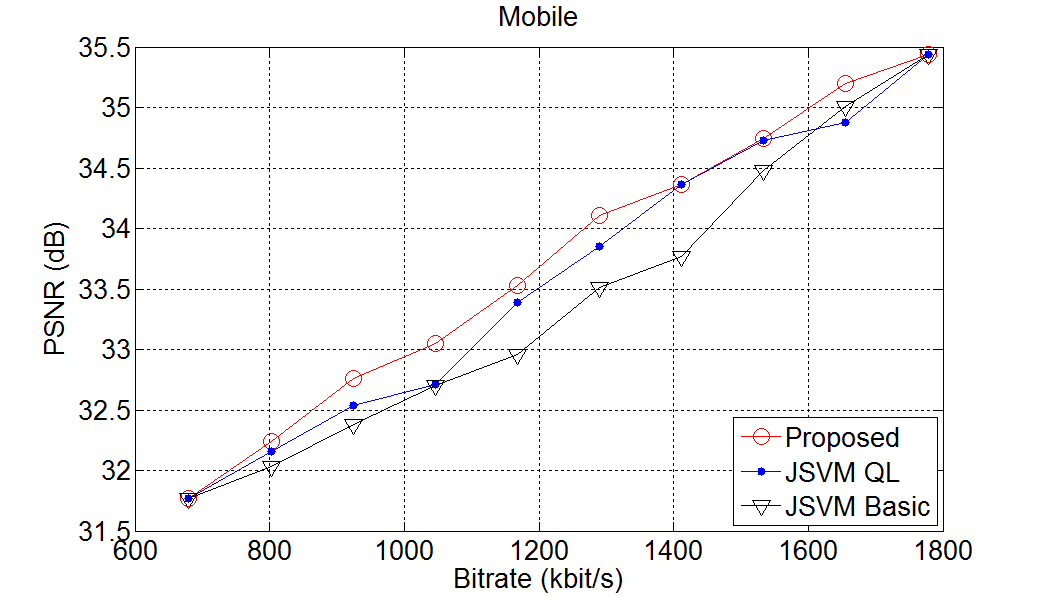
\includegraphics[width=0.5\textwidth]{figures/Mobile-noref.png}}
	\subfloat[Soccer]{
		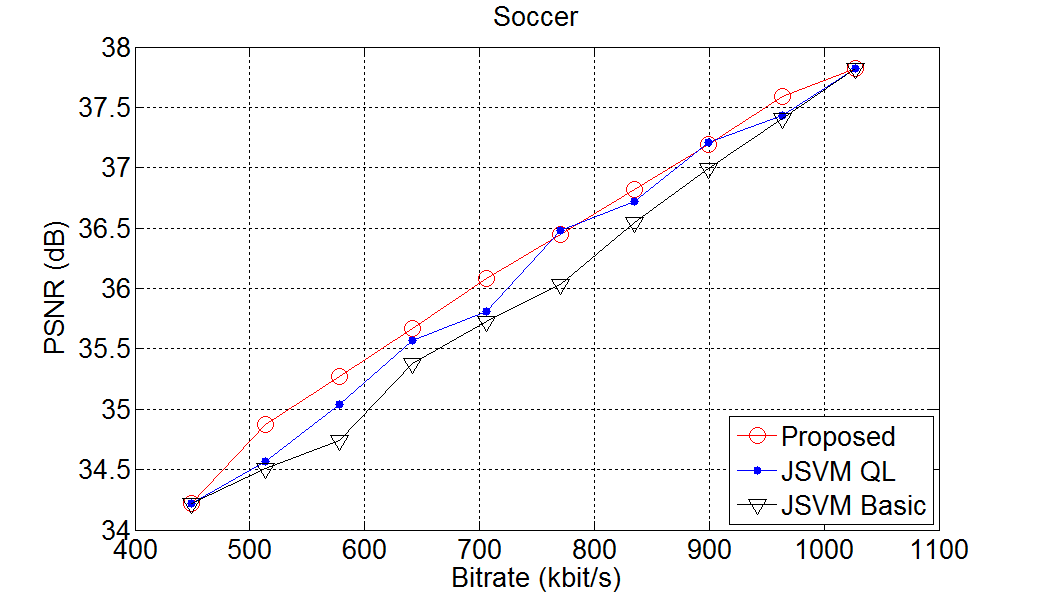
\includegraphics[width=0.5\textwidth]{figures/Soccer-noref.png}}
	\caption{无参考源时三种码流截取方案的性能比较}
	\label{fig:extraction-performance-noref}
\end{figure*}

对于无参考源的应用场景,我们也做了相应的实验。图\ref{fig:extraction-performance-noref}展示了全部八个测试序列在无参考截取实验中的性能比较结果,直观地表明了本文所提方案取得了较好的率失真性能。表\ref{tab:extraction-gain-noref}列出了对应的PSNR提升数据,同样可以看出本文所提出的方案的优越性。

为了进一步证明本文提出的码流截取方案在无参考情况下的有效性,我们除了与JSVM对比,还做了进一步的对比实验。比较对象一方面选了Maani等人的方法\supercite{Maani2009},另一方面选了不进行本文\ref{subsec:noref}小节中的修改而直接采用公式(\ref{eq:R-D_impact_i})的方法。由于Maani等人的方法所取得的结果取决于其训练出的模型参数,为了公平起见,我们控制了训练过程的计算量,使其与我们的方法计算复杂度相同。表\ref{tab:methods-compare}列出了三种不同的无参考截取方法相对于JSVM QL的平均PSNR提升。可以看出,Maani等人的方法在无参考情况下跟本文的方法性能相差无几,而在进行本文\ref{subsec:noref}小节中的修改之前,直接采用公式(\ref{eq:R-D_impact_i})则性能差了许多,甚至在有些序列上取得了比JSVM QL还差的结果。这进一步说明了\ref{subsec:noref}小节中修改的重要性。

\begin{table*}[!ht]
	\centering
	\vspace{10pt}
	\caption{无参考源时本文提出的截取方案相比于JSVM的PSNR提升}
	\label{tab:extraction-gain-noref}
	\small
	\begin{minipage}{1.0\linewidth}
		\centering
		\begin{tabular}{c|c|*{3}{p{0.9cm}<{\centering}|}*{4}{p{1.1cm}<{\centering}|}p{0.9cm}<{\centering}}
			%% |l|l| to left justify each column entry
			%% |c|c| to center each column entry
			%% use of \rule[]{}{} below opens up each row
			\hline \hline
			\multicolumn{2}{c|}{序列名} &
			{\em Bus} & {\em City} & {\em Crew} & {\em Football} & {\em Foreman} & {\em Harbour} & {\em Mobile} & {\em Soccer} \\ \hline 
			\multirow{2}{*}{JSVM QL, $K$ = 32 \footnote{\label{footnote:JSVM_QL-noref} 与JSVM QL对比;优化窗口大小为32帧}}
			& Max\footnote{\label{footnote:max-noref} 所有码率限制下的最大提升}
			& 0.36 & 0.56 & 0.41 & 0.31 & 0.45 & 0.30 & 0.34 & 0.30 \\ \cline{2-10}
			& Ave\footnote{\label{footnote:ave-noref} 所有码率限制下的平均提升}
			& 0.14 & 0.22 & 0.13 & 0.12 & 0.17 & 0.11 & 0.14 & 0.11 \\ \hline
			\multirow{2}{*}{JSVM Basic, $K$ = 32}
			& Max & 0.48 & 0.97 & 0.54 & 0.25 & 0.47 & 0.38 & 0.60 & 0.53 \\ \cline{2-10}
			& Ave & 0.23 & 0.48 & 0.23 & 0.12 & 0.28 & 0.21 & 0.31 & 0.26 \\ \hline
		\end{tabular}
	\end{minipage}
\end{table*}

\begin{table*}[!ht]
	\centering
	\vspace{10pt}
	\caption{不同的无参考截取方法对比:相对于JSVM QL的平均PSNR提升}
	\label{tab:methods-compare}
	\small
	\begin{minipage}{1.0\linewidth}
		\centering
		\begin{tabular}{c|*{3}{p{0.9cm}<{\centering}|}*{4}{p{1.1cm}<{\centering}|}p{0.9cm}<{\centering}}
			\hline \hline
			序列名 & {\em Bus} & {\em City} & {\em Crew} & {\em Football} & {\em Foreman} & {\em Harbour} & {\em Mobile} & {\em Soccer} \\ \hline
			本文方法  & 0.14 & 0.22 & 0.13 & 0.12 & 0.17 & 0.11 & 0.14 & 0.11 \\ \cline{1-9}
			Maani等人的方法\supercite{Maani2009} & 0.13 & 0.22 & 0.13 & 0.11 & 0.16 & 0.02 & 0.08 & 0.12 \\ \cline{1-9}
			采用公式(\ref{eq:R-D_impact_i})方法 & 0.06 & 0.07 & 0.01 & 0.10 & 0.05 & 0.04 & -0.03 & -0.01 \\ \hline
		\end{tabular}
	\end{minipage}
\end{table*}

\section{本章小结}

本章介绍了一个采用线性误差模型的可伸缩视频码流截取方案。我们从H.264/AVC解码过程的线性性质推导出了质量可伸缩情况下的线性误差模型。该模型能使我们准确地估计丢弃任意数据包所带来的失真变化。基于此,我们设计了一个贪心算法来根据数据包的码率失真影响来为其赋优先级值,并按照这些优先级值来进行码流截取。实验表明,本文提出的线性误差模型对失真估计的误差率只有5\%,而采用该模型的码流截取相比于参考软件中的截取器有高达0.5dB的PSNR提升。本章的工作使得视频流媒体的数据源能够以很高的精度改变码率,为下一章要介绍的码率自适应提供了条件。
	\chapter{基于PID控制思想的码率自适应算法}

在实际网络环境中,带宽波动是不可避免的。对于一个视频流媒体系统而言,只有根据带宽变化来自适应地调整发送码率才能为用户提供更好的服务。在上一章中,我们通过可伸缩视频的码流截取,使得码率能够调整;在本章中,我们主要关注如何调整。由于视频码率与视频质量一般来说是直接相关的(高码率对应高质量),调整码率也就是调整所传送视频的质量。因此,本章所解决的问题又被称为质量控制问题。我们将基于经典控制实践中的PID思想,设计一个综合考虑带宽的历史状况、当前状态和未来趋势的码率自适应算法,从而提高发送视频的总体质量和平滑度。

\section{PID控制器简介}

PID控制器\footnote{http://en.wikipedia.org/wiki/PID\_controller}是一个在工业控制系统中常用的闭环反馈控制器。PID控制中的两个重要概念是过程变量和控制目标。过程变量代表着系统当前的状态,而控制目标是系统希望达到的理想状态。PID控制的基本思想就是根据过程变量和控制目标之间的误差来确定一个控制输出,该输出反馈作用到系统以最小化上述误差。

PID控制器的控制输出一般如下定义:
\begin{equation}
\label{eq:pid-output}
u(t) = {K_p} \cdot e(t) + {K_i} \cdot \int_0^t {e(\tau )d\tau }  + {K_d} \cdot \frac{d}{{dt}}e(t) \: ,
\end{equation}
其中$e(t)$指代过程变量与控制目标在时刻$t$的误差,$K_p$、$K_i$、$K_d$是三个可调参数,依次称为比例增益、积分增益和微分增益。公式(\ref{eq:pid-output})的结果通过某种方式来影响系统状态,使得过程变量朝着控制目标变化。

作为一个灵活有效的控制技术,PID可以被用来解决各种各样的控制问题\supercite{Wong2004}\supercite{Li1999}。在本文的工作中,我们基于它设计了一个码率自适应算法,用来控制视频流媒体中的视频质量。

\section{基于PID的码率自适应}

本节首先介绍质量等级的概念,将视频流媒体中的视频质量和码率值离散化,接着定义在所提出的码率自适应算法中用到的过程变量及其控制目标。之后,我们详细解释控制模型和算法流程,并简要讨论PID参数的选取和调优。

\subsection{质量等级划分}

视频质量或码率是一个连续的值,以任意的精度来控制或调整它是不现实的。因此,我们首先提出一个质量层级的概念来离散化视频质量和码率。当需要调整时,我们只是增加或减少质量等级。每一个质量等级对应一个确定的码率。高等级对应高码率,反之亦然。有多少个质量等级以及它们跟具体码率值如何对到应可以根据实际需求来确定。质量等级越多,系统就能越精细地调整码率来适应带宽变化。如绪论中所说,用多码流实现的自适应流媒体系统只能提供有限的几个质量等级,而基于可伸缩视频编码的流媒体系统能够以更高的精度来定义质量等级。

\subsection{过程变量和控制目标}

在本文所提出的质量控制算法中,所选取的过程变量称为“实际与检测间隔比”。下面介绍其具体定义。

\begin{figure}[h]
	\centering
	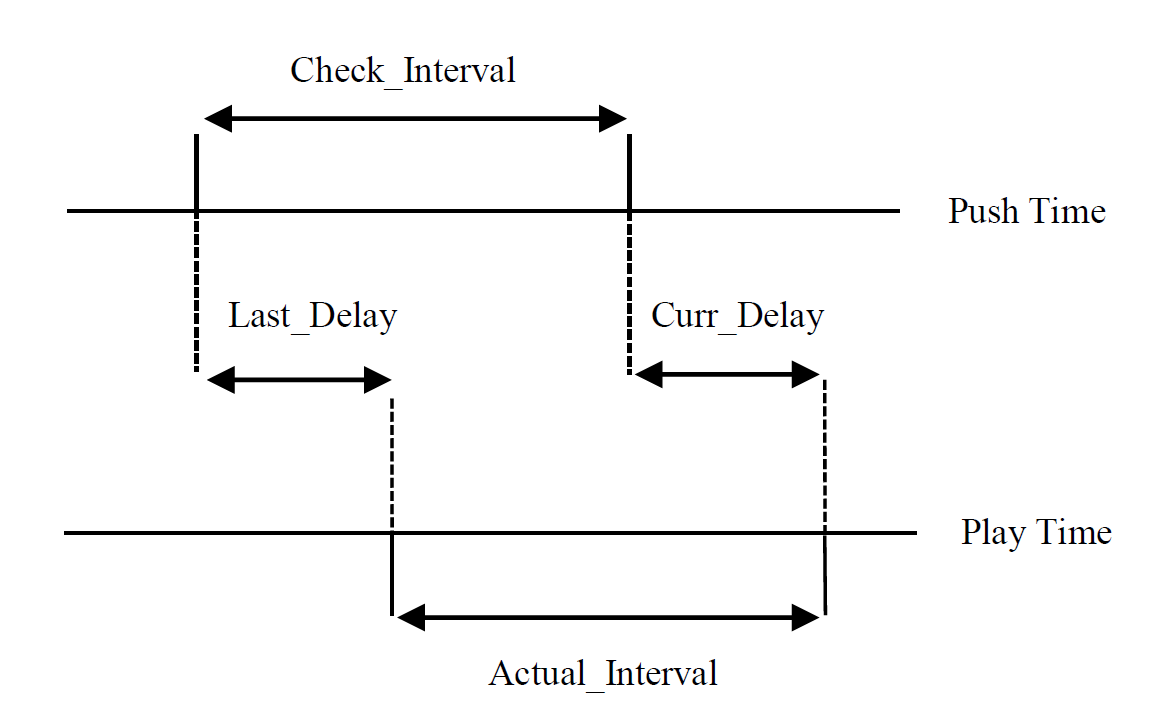
\includegraphics[width = 0.9\linewidth]{figures/Intervals.png}
	\caption{达尔文流媒体服务器中的两个时间线 \label{fig:intervals}}
\end{figure}

在达尔文流媒体服务器中,有两个时间线非常重要。第一个是推送时间线(push time),也就是视频数据包被推送到缓冲区的时间;第二个是播放时间线(play time),也就是数据包应该在播放中被显示的时间(通常记作该数据包的PTS)。这两个时间线的关系如图\ref{fig:intervals}所示。服务器程序会定时检测这两个时间线,并根据数据包的延迟来决定是否需要调整发送的视频质量。图\ref{fig:intervals}中的两个间隔,即检测间隔(check interval)和实际间隔(actual interval),值得我们注意。在理想情况下,每次检测间隔中服务器推送的数据量应该恰好能实际播放等于检测间隔的一段时间,也就是\textit{actual\_interval} = \textit{check\_interval}。如果实际间隔小于检测间隔,说明这段时间内推送了较少的数据,推送数据变慢很可能是带宽有所下降。反过来,如果实际间隔大于检测间隔,说明这段时间内推送了较多的数据,意味着网络条件良好且数据被快速推向客户端。这两个间隔的比值,也就是所谓的“实际与检测间隔比”,能够反映当前推送的速率是否与网络带宽相符。

“实际与检测间隔比”适合用作质量控制有三方面的原因。第一,这个比例直接对应着适合带宽的码率与当前传输的码率的比值,只需据此进行调整就可以准确地使码率符合带宽。第二,根据定义这个比例的理想值就是1,这就是算法的控制目标,无需再通过别的方法确定。第三,这个值在实际系统中便于计算,普适性较好。

\subsection{控制模型和算法描述}

在通常的PID控制器中,控制输出是用过程变量与控制目标之间的差值进行比例、积分、微分求取出来的。考虑到我们所选的过程变量是一个比例,且控制目标是1,本文对通常的PID控制器做了修改,提出了一个基于比例的模型。在这个模型中,过程变量直接被用来计算控制器输出,而且所有求差的运算都被适当的改为了求比例的运算,以保持模型的合理正确性,如下所示:

\begin{equation}
\label{eq:ut}
{u_t} = {K_p} \cdot E_p^t + {K_i} \cdot E_i^t + {K_d} \cdot E_d^t ,
\end{equation}

\begin{equation}
\label{eq:ep}
E_p^t = \frac{{actual\_interva{l_t}}}{{check\_interva{l_t}}} ,
\end{equation}

\begin{equation}
\label{eq:ei}
E_i^t = \frac{{long\_actual\_interva{l_t}}}{{long\_check\_interva{l_t}}} ,
\end{equation}

\begin{equation}
\label{eq:ed}
E_d^t = E_p^t/E_p^{t - 1} ,
\end{equation}

\begin{equation}
\label{eq:long-actual}
long\_actual\_interva{l_t} = \sum\limits_{\tau = {T_l}}^t {actual\_interva{l_\tau}} ,
\end{equation}

\begin{equation}
\label{eq:long-check}
long\_check\_interva{l_t} = \sum\limits_{\tau = {T_l}}^t {check\_interva{l_\tau}} .
\end{equation}

在公式(\ref{eq:ut})中:$K_p$、$K_i$、$K_d$分别表示比例部分、积分部分、微分部分的可调参数;$E_p^t$、$E_i^t$、$E_d^t$则对应各部分在第t次检测时的值,它们的定义如公式(\ref{eq:ep})至(\ref{eq:long-check})所示;控制器输出$u_t$将用来计算适合当前带宽的码率,并据此选择要传送的质量等级。

在公式(\ref{eq:long-actual})和(\ref{eq:long-check})中,$T_l$代表上一次质量等级改变的时间。按照理论定义,积分部分应该从系统启动开始记录,但在实际环境中,网络带宽有可能变动非常大,如果积分部分记录累积太长时间将不适合反映当前的网络条件,从而减缓调整质量的决策。因此这里采用了一个折衷,选择从上一次质量等级变化的时间开始计算积分部分。

这个基于比例的模型对于所选的过程变量和控制目标比通用模型更加简单有效。而且,在该模型中,当三个参数进行归一化处理后,控制器输出具备明显直观的意义。从公式(\ref{eq:ep})至(\ref{eq:long-check})容易看出,$E_p^t$、$E_i^t$、$E_d^t$这三个值都是在1附近波动的比值;而根据公式(\ref{eq:ut}),控制器输出$u_t$可以被视作这三个比值的加权平均(三个参数作为权值)。因此,$u_t$也是一个在1附近的比值,它对应着适合当前带宽的码率与当前发送码率的关系。换句话说,如果$u_t$大于1,那么控制器决定当前发送码率需要增加;反之,如果$u_t$小于1,意味着控制器认为当前发送码率需要减小。用$u_t$作为一个乘子来调整当前发送的码率,我们就能控制流媒体系统符合带宽的变化。

本文提出的码率自适应算法描述如Algorithm\ref{algo:control}所示。相比于其他的调度策略,这个基于PID的自适应算法具有以下几个优点。首先,该算法不仅仅依据当前状态或者固定时间点的信息来做决策,因此质量调整可以在任何合适的时间发生。其次,因为PID模型(微分部分)在某种程度上考虑了对未来的预测,该算法能够判断带宽在未来一段时间内是否会变得足够大或足够小,因此能避免一些不必要的调整。最后,该算法并不一定一次只调整一个质量等级,这就使得当带宽剧烈下降时能够快速下调质量以保证流畅播放,而当系统启动时能够快速上调质量以使用户尽早收到更清晰的视频。

\begin{algorithm}
	\caption{基于PID的码率自适应算法}
	\label{algo:control}
	\begin{algorithmic}
		\STATE 准备发送数据包
		\STATE check\_interval = curr\_time -- last\_check\_time
		\STATE actual\_interval = curr\_media\_time -- last\_check\_media\_time
		\STATE long\_check\_interval += check\_interval
		\STATE long\_actual\_interval += actual\_interval
		\STATE 根据公式(\ref{eq:ep}) - (\ref{eq:ed})计算$E_p^t$、$E_i^t$、$E_d^t$的值
		\STATE output = ${K_p} \cdot E_p^t + {K_i} \cdot E_i^t + {K_d} \cdot E_d^t$
		\STATE new\_bitrate = output * curr\_bitrate
		\STATE new\_level = get\_level(new\_bitrate, bitrate\_of\_level[])
		\IF {质量等级变化}
		\STATE long\_check\_interval = 0
		\STATE long\_actual\_interval = 0
		\STATE curr\_bitrate = bitrate\_of\_level[new\_level]
		\ENDIF
		\STATE 根据新的质量等级发送数据包
	\end{algorithmic}
\end{algorithm}

\subsection{参数选取与调优}

与工业界的其他PID控制系统一样,本文提出的算法中三个参数的选取也是跟具体实现相关的。大多数情况下,为取得最优的效果,需要手动试错调节。每个参数对系统的不同方面产生影响,知道这些影响有助于进行参数选取。一般来说,PID控制器中的比例部分会影响系统的稳定性。如果比例增益$K_p$过高,系统容易变得不稳定。但是,太低的$K_p$又会导致过长的上升时间,使系统响应迟缓。积分部分除了能消除稳态误差,还能加速过程变量向控制目标的变化。这意味着,增大$K_i$能减小上升时间,提高系统的响应速度。但是,积分部分会累积过去一段时间的误差,使过程变量容易超出目标值(即超调),因此过大的$K_i$也会导致系统不稳定。上述这些隐患都能通过微分部分来校正。微分部分通过预测系统行为,具有减小超调、提高稳定性的双重效果。但是微分部分的特点是对误差分成敏感,也正是因为此,工业实践中微分增益$K_d$通常都设置的比较低。

本文采用了经典的Ziegler--Nichols方法\supercite{Ziegler1942}来进行参数选取。该方法首先把积分和微分参数设为0,调节比例参数$K_p$到系统开始震荡时的值$K_u$,假设震荡周期为$T_u$,那么设置$K_p = 0.6K_u$、$K_i = 2K_u/T_u$、$K_d = K_u \cdot T_u/8$。再将$K_p$、$K_i$和$K_d$进行归一化,就得到最终的参数:$K_p = 0.22$,$K_i = 0.73$,$K_d = 0.05$。在这样的参数配置下,由本文提出的算法所控制的流媒体系统是稳定的,而且能够很快开始适应带宽的变化,具体参见下一节中的实验结果。

\subsection{扩展应用到直播系统}

PID控制思想具有很强的扩展性,除了上述在达尔文流媒体点播中的应用,我们还将其用在了直播系统中。本小节对这一扩展应用进行介绍,重点是说明点播系统与直播系统的不同之处,以及如何选取合适的过程变量和控制目标。

在有些视频直播系统中,视频内容由服务器或者与服务器通过局域网连接的设备生成,在这种情形下,视频直播和视频点播具有很多共同点。在直播中服务器将动态生成的视频数据发送给客户端,和点播最主要的区别在于传输速率不能超过视频数据生成速率,因此当所有生成的数据都传输之后,客户端需要等待下一个数据片段就绪\supercite{Thang2014}。而在如今十分火热的用户生成内容(UGC)直播模式下,服务器本身不充当初始的内容产生方,在其他设备上持续生成的视频内容经过不确定且不可忽略的延迟传输到中转服务器。目前已经分成普及的智能手机成为了理想的内容产生方和接收方。图\ref{fig:07}展示了通用的手机视频直播系统的主要模块。集成了高效视频编码器的智能手机,将实时视频数据传输到接收服务器,在此同时,原始视频流被转码成多路具有不同码率的视频流。客户端可以通过当前网络环境选择最合适的码率,从服务器获取视频数据。

\begin{figure}[h]
	\centering
	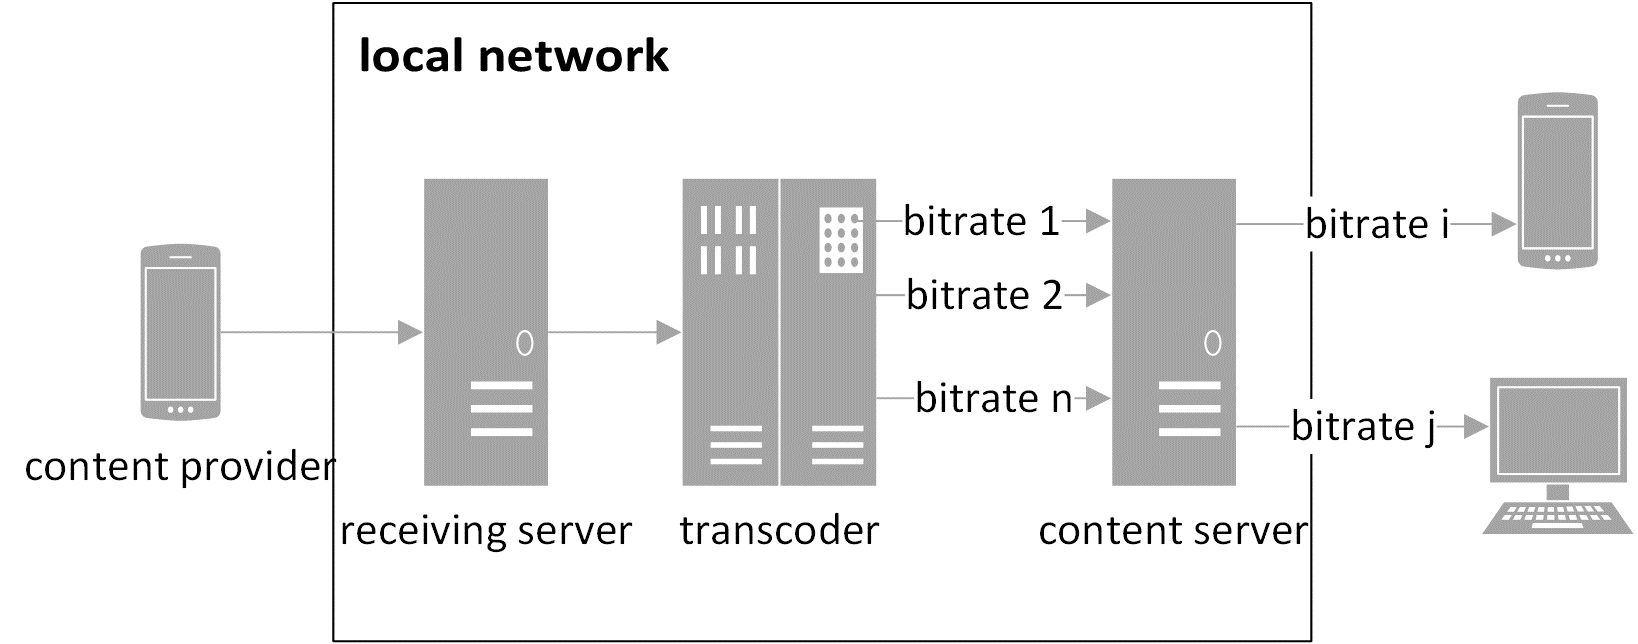
\includegraphics[width = 1.0\linewidth]{clip/07.png}
	\caption{通用的手机直播系统模型\label{fig:07}}
\end{figure}

为了提供高质量的直播视频流,内容产生方需要传输尽可能高码率的视频,这可能导致每个数据段传输时间过长,造成接收端的播放中断。而内容产生方在变化的网络状况下尽可能利用网络吞吐量传输高质量视频的同时保证接收端的流畅播放,是一个挑战。与此同时,延迟需要控制在一个可以接收的范围。我们在内容产生方设计了一个上传码率自适应控制器,这种方案能够应用于UGC的视频直播。

简单起见,我们假设服务器具有快速的内部操作,同时接收端通过稳定高效地网络与服务器进行连接,这意味着服务器和接收端的视频流与内容产生方和服务器的视频流保持同步。这个假设对我们的研究重点没有影响。我们将传输架构简化成如图\ref{fig:08}所示。内容产生方的编码器将输入视频压缩之后传递给基于TCP的应用层协议。经过各层协议的封装,数据被传递到网络进行实际传输。在接收端经过一个逆向过程之后,数据输入到解码器进行解码,然后在播放器中进行渲染。与此同时,在发送方的自适应控制器每隔特定的周期对传输信息进行检查,并采用后文将介绍的特定的策略对编码器参数进行调整。

\begin{figure}[h]
	\centering
	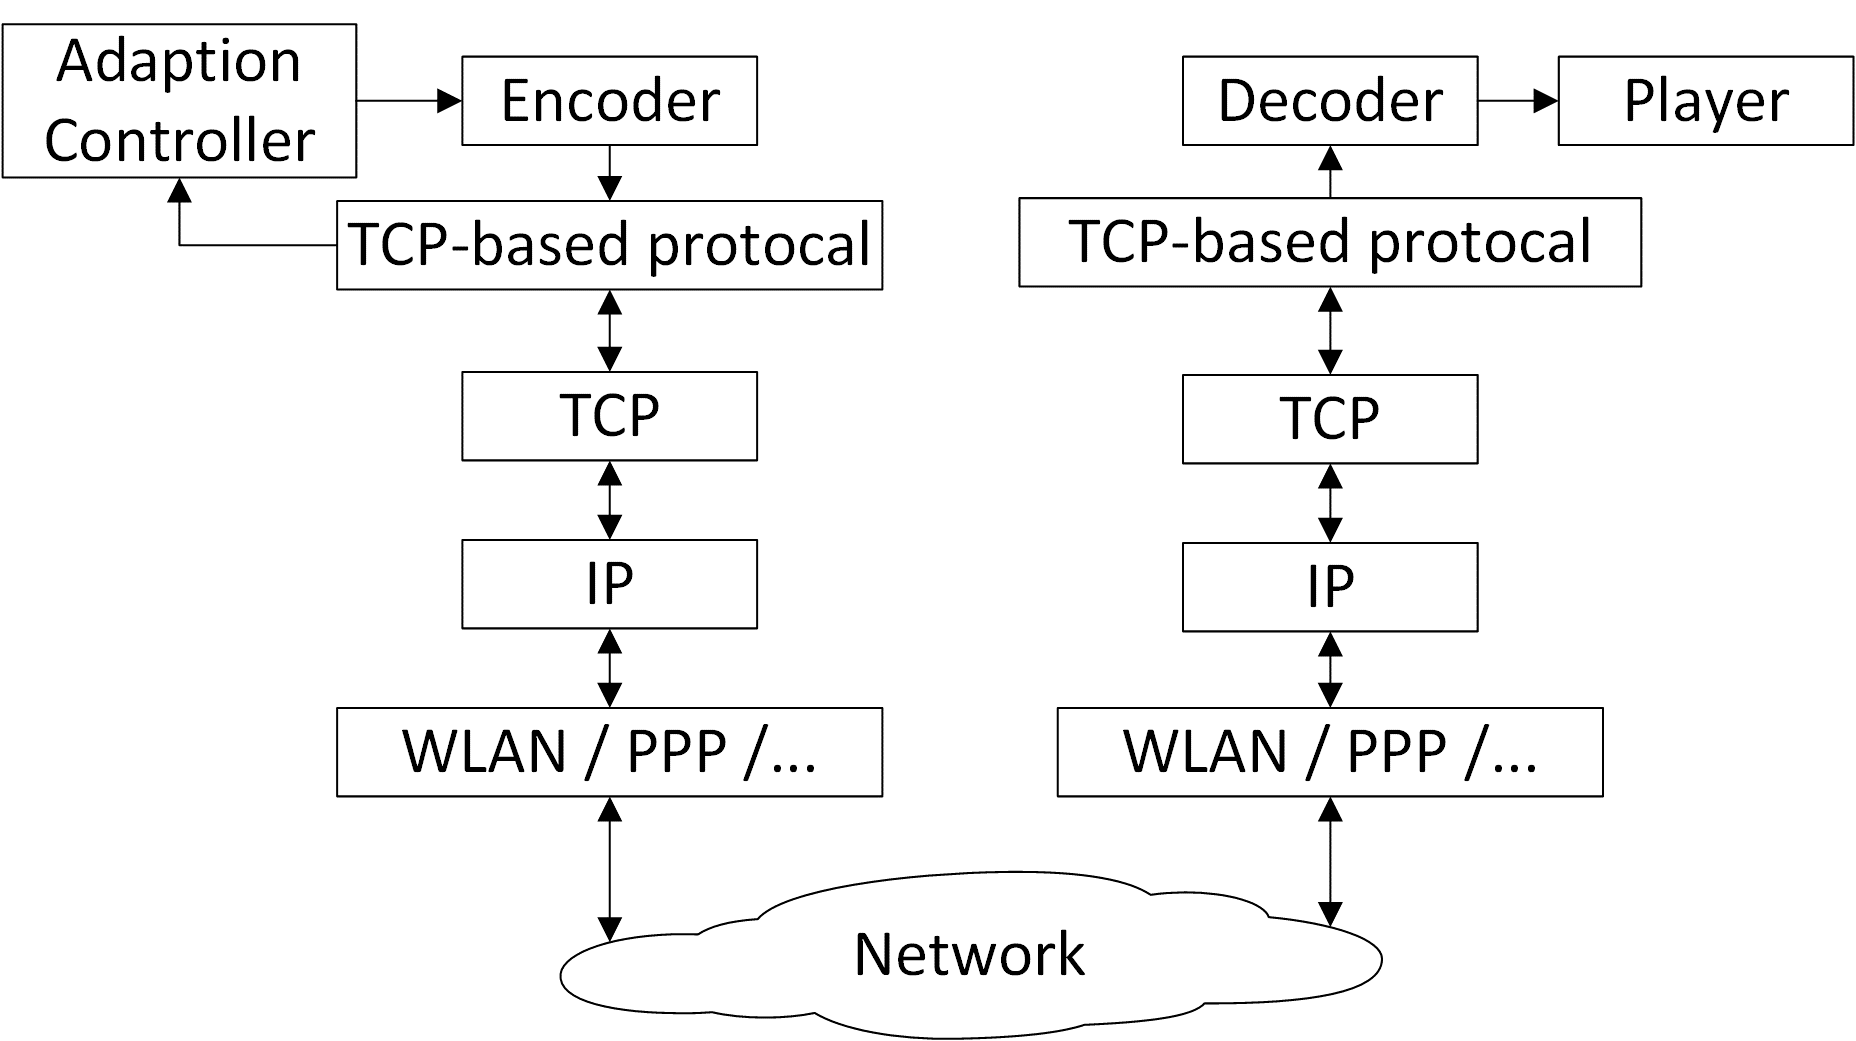
\includegraphics[width = 1.0\linewidth]{clip/08.png}
	\caption{简化直播系统传输架构\label{fig:08}}
\end{figure}

使用PID进行码率自适应的关键在于选取一个能够反映传输状况的过程变量。基于TCP的直播系统在传输过程中有四个缓冲区,分别是应用层发送缓冲区(ASB)、TCP发送缓冲区、TCP接收缓冲区、播放缓冲区(PB)。其中对内容产生方最重要的信息是ASB内的数据长度,记为择$S_{ASB}(t)$(在时刻$t$的值),它能够直接反映视频码率和吞吐量之间的匹配情况。当视频码率高于当前的吞吐量时,该缓冲区内的数据长度趋向于增大,否则保持相对稳定或者减小为0。理想状况下,它首先应该是一个大于0的值,以保证接收方播放不中断;其次它不应该太大,否则意味着发送码率太高。所以,我们选择$S_{ASB}(t)$作为系统的过程变量,而选择一个接近0的常量$\varepsilon$作为控制目标。

然而,如果网络吞吐量在一个小的范围频繁波动,将使得系统变量值不稳定而且相对随机,导致不必要的频繁的调整。为了消除这样的随机性,我们将过程变量的定义修改为$\overline{S_{ASB}(t)}$,它表示在时刻$t$之前的一个时间段$\tau$内$S_{ASB}(t)$的平均值。它可以表示为:
\begin{equation}
\label{eq:asb}
\overline{S_{ASB}(t)} = \dfrac{1}{\tau} \int_0^\tau {S_{ASB}(t)}\: .
\end{equation}

对于UGC直播应用来讲,由于发送的码流是实时生成的,所以调整码率时直接改变编码器参数以改变生成码率即可,不需要涉及码流截取等数据源端的操作。但是,质量等级的概念仍然需要,它在这里变成了改变码率的单位。控制模型可以直接采用原始PID中的做法,用过程变量和$\varepsilon$的差值来计算比例、积分、微分这几个部分。具体的算法流程以及三个PID参数的选取和调优与上一小节中的相同,这里不再详述。

\section{实验结果}

\subsection{用伸缩层组合定义的质量等级}

为了简单起见,在第一部分实验中,我们先用可伸缩视频内置的伸缩层级组合成质量等级来用于质量控制。该定义的基本思想是将视频码流中的数据包分成若干组。分组的依据是这个数据包所属的伸缩层,也就是储存在NALU头信息中的层ID字段。表\ref{tab:sub-stream}展示了组ID与层ID的对应关系。我们所用的测试码流含有3个质量层和3个时间层,因此其中的数据包被分为9个组。质量等级被定义为组ID不大于等级值的所有组的合集。例如,质量等级2含有组0到组2内的所有数据包,因此将包含所有的时间层,但只有质量基本层;质量等级5含有组0到组5,于是将进一步包括第一个质量增强层的数据包。类似这样,随着质量等级的升高,越来越多的增强层数据包被累积进来,视频质量逐渐提升;与此同时,码率也越来越高,因为更好的质量显然需要更高的码率。我们测试用的完整码流码率是1587kbps,对应着最高的质量等级。这样用伸缩层来构造质量等级可以不用额外的数据,只需解析码流中本来已经包含的层ID即可,实现起来比较简单。

\begin{table*}[h]
\centering
\caption{质量等级定义中组ID与层ID的对应关系}
\label{tab:sub-stream}
\begin{tabular}{c|*{8}{p{1.0cm}<{\centering}|}{p{1.0cm}<{\centering}}}
	\hline\hline
	  组ID   & 0 & 1 & 2 & 3 & 4 & 5 & 6 & 7 & 8 \\ \hline
	质量层ID  & 0 & 0 & 0 & 1 & 1 & 1 & 2 & 2 & 2 \\ \hline
	时间层ID & 0 & 1 & 2 & 0 & 1 & 2 & 0 & 1 & 2 \\ \hline
\end{tabular}
\end{table*}

\subsection{实验配置}

在我们的实验中用限速软件NetLimiter\footnote{http://www.netlimiter.com/}来模拟实际网络环境中的带宽情况。平均带宽的取值从400kbps到1400kbps,以100kbps的间隔递增。对于每个平均带宽值,通过在平均值基础上加随机干扰来模拟带宽波动。在带宽波动的情况下,流媒体系统在每种质量控制算法下各运行10分钟,并记录所发送的质量等级变化。所有质量等级的平均值作为视频质量的度量,而所有质量等级的方差作为质量平滑性的度量。这两个指标被用于不同算法的比较。比较中的基准算法是达尔文流媒体服务器中内置的包延迟反馈(packet delay feedback,简称PDF)算法。

接下来,我们展示各种质量控制算法的结果并进行分析比较。

\subsection{结果和分析}

为了分析PID控制模型各个部分的效果,我们首先只用比例部分和积分部分来进行了初步的测试实验。由于这两个部分各自对应当前的短期误差和积累的长期误差,我们分别称之为短期预测算法(short-term prediction,简称STP)和长期预测算法(long-term prediction,简称LTP)。图\ref{fig:performance-all}展示了这两种控制算法和基准算法的实验结果。可以看出,短期预测算法能取得最高的平均质量等级,但它的质量等级方差也是最高的。这正符合短期预测总是倾向于紧紧跟随带宽变化的特点。长期预测算法恰恰与之相反,保持了一个较低的质量等级方差,但也牺牲了一部分平均质量。虽然它的平均质量不如短期预测算法,但也超出了基准算法。

\begin{figure*}[t]
\centering
\subfloat[不同质量控制算法的质量等级均值]{
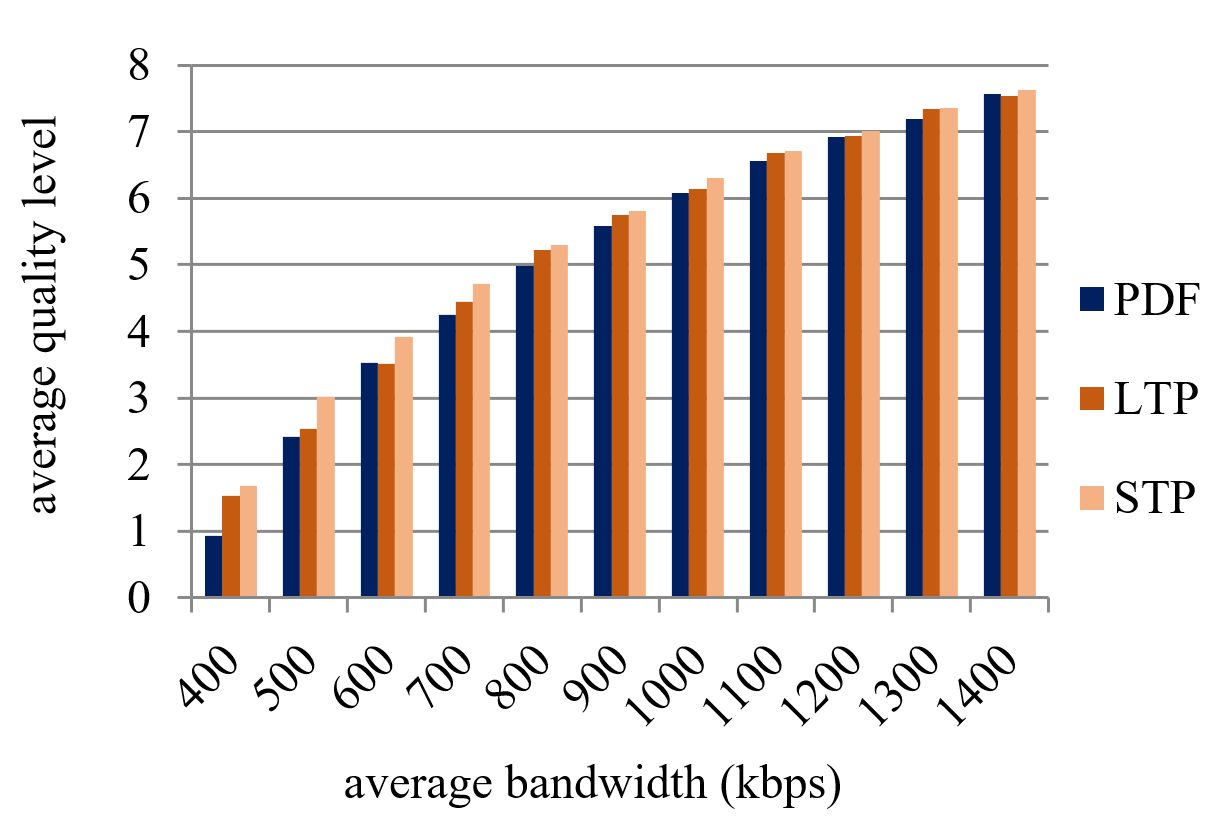
\includegraphics[width=0.5\textwidth]{figures/Quality-all.png}
\label{fig:quality-all}}
\subfloat[不同质量控制算法的质量等级方差]{
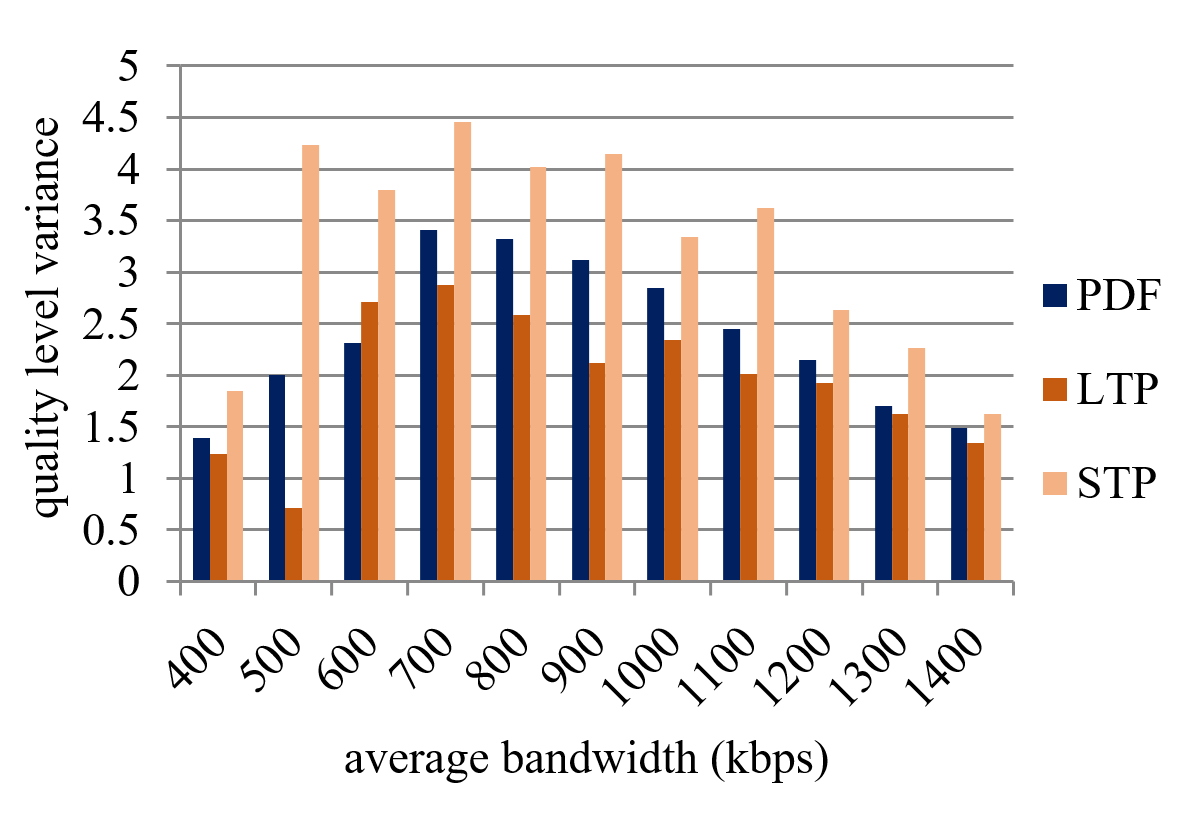
\includegraphics[width=0.5\textwidth]{figures/Variance-all.png}
\label{fig:variance-all}}
\caption{长/短期预测算法与达尔文服务器中的包延迟反馈(PDF)算法的比较}
\label{fig:performance-all}
\end{figure*}

\begin{figure*}[t]
\centering
\subfloat[PID和PDF算法的质量等级均值]{
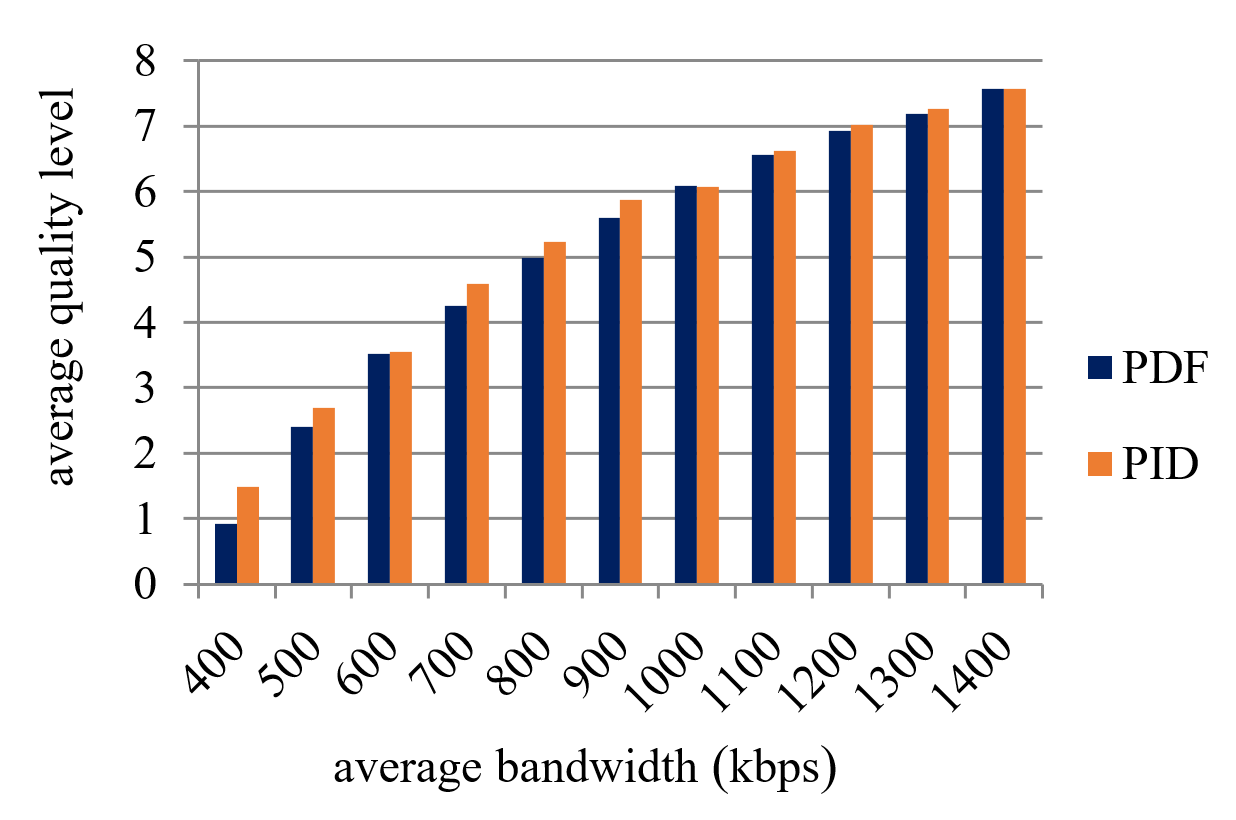
\includegraphics[width=0.5\textwidth]{figures/Quality-two.png}
\label{fig:quality-two}}
\subfloat[PID和PDF算法的质量等级方差]{
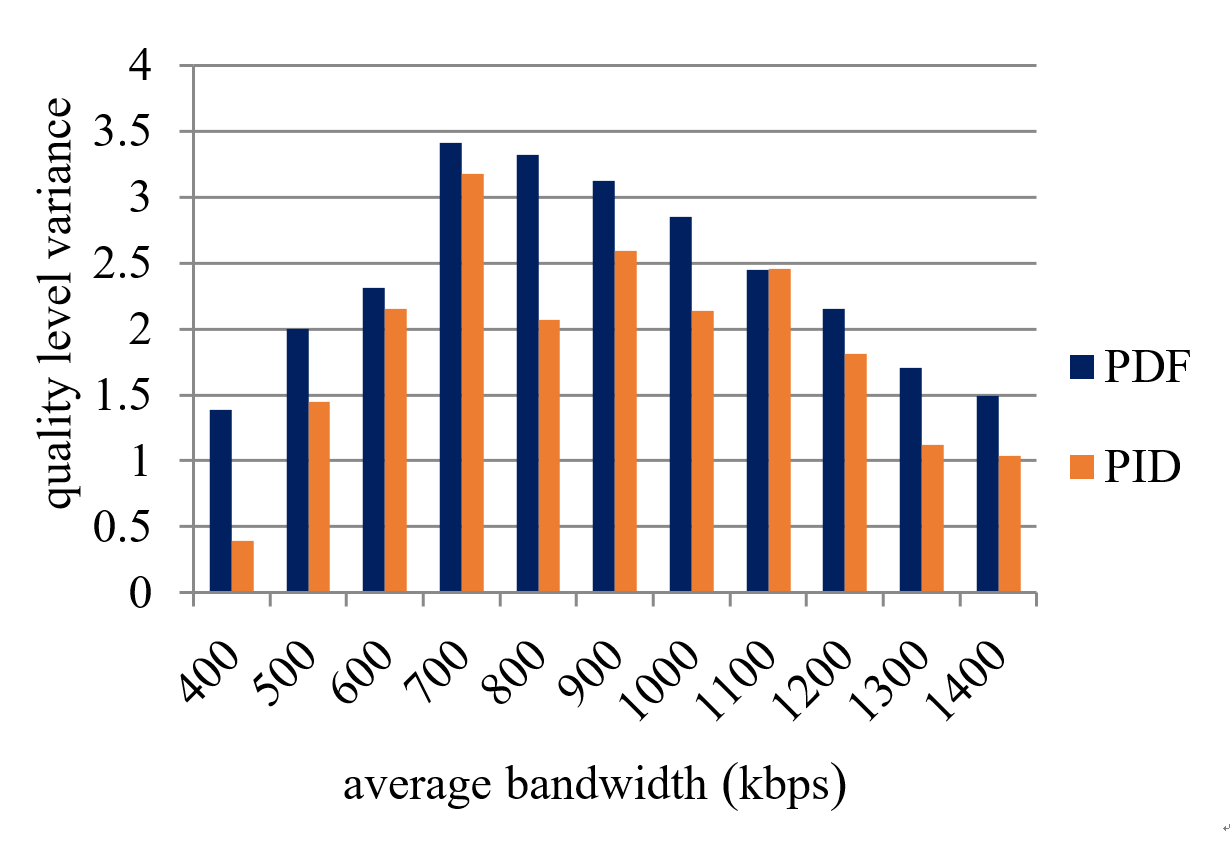
\includegraphics[width=0.5\textwidth]{figures/Variance-two.png}
\label{fig:variance-two}}
\caption{本文提出的PID控制算法与达尔文服务器中的包延迟反馈(PDF)算法的比较}
\label{fig:performance-two}
\end{figure*}

短期预测和长期预测算法有各自的局限性,完整的PID控制算法则既能降低质量波动又能提升平均质量。实验结果可参见图\ref{fig:performance-two}。可以看到,当与积分和微分相结合后,比例部分在短期预测算法中那样的激进效果已经弱化了。如图\ref{fig:variance-two}所示,PID算法取得了比PDF算法更低的质量波动。

表\ref{tab:improvement}列出了四种控制算法的定量比较数据,从中我们可以看出PID算法相比其他几种算法有明显的优势。与基准算法PDF相比,基于PID的质量控制算法取得了8.6\%的视频质量提升,同时将质量波动也降低了24.8\%。当带宽在平均值800kbps附近波动的时候,四种控制算法对应的视频质量等级变化情况如图\ref{fig:fluctuation}所示。从中我们可以明显观察到PID控制算法得到的视频质量更加平稳。

\begin{table*}[h]
\centering
\caption{不同质量控制算法与包延迟反馈算法的定量比较}
\label{tab:improvement}
\begin{tabular}[b]{p{4.2cm}<{\centering}|p{4.2cm}<{\centering}|p{4.2cm}<{\centering}}
\hline \hline
控制算法 & 质量等级均值的增长 & 质量等级方差的增长 \\ \hline
包延迟反馈 (PDF) & 0.0\% & 0.0\% \\ \hline
短期预测 (STP) & \textbf{+13.5\%} & +38.5\% \\ \hline
长期预测 (LTP) & +7.9\% & -17.2\% \\ \hline
PID控制 (PID) & +8.6\% & \textbf{-24.8\%} \\ \hline
\end{tabular}
\end{table*}

\begin{figure}
\centering
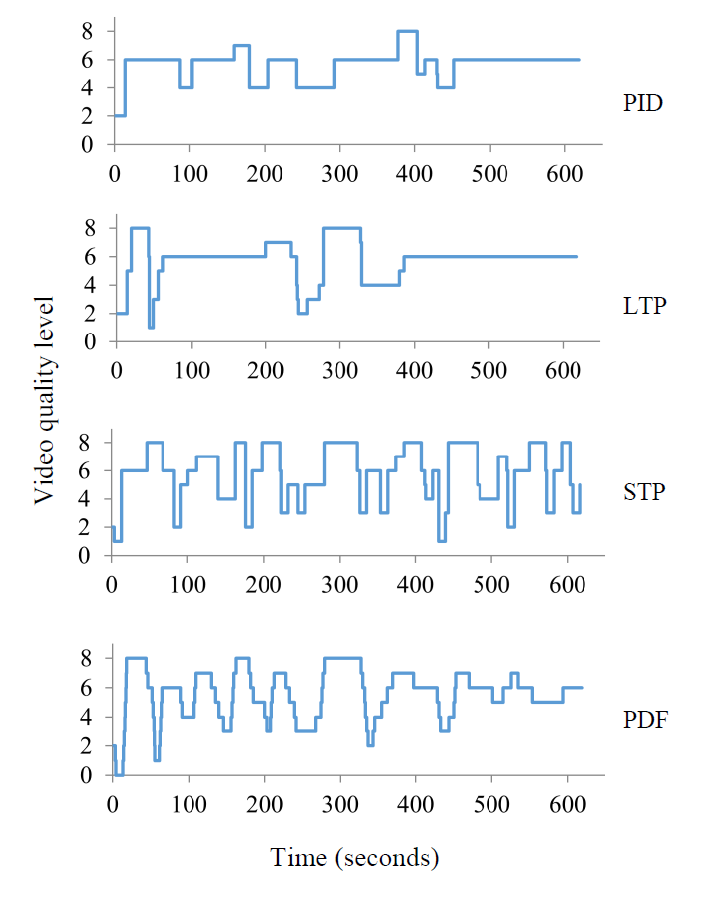
\includegraphics[width = 0.45\linewidth]{figures/Fluctuation.png}
\caption{不同质量控制算法下视频质量等级随时间的变化情况 \label{fig:fluctuation}}
\end{figure}

\subsection{与码流截取相结合的效果}

上面的实验直接用可伸缩视频中内置的伸缩层来构造质量等级,并没有结合本文前一章中提出的码流截取算法。实际的可伸缩视频流媒体系统中,当码率自适应算法给出一个适合传输的码率后,由码流截取方案根据这一码率限制截取出一个子流向客户端发送。本小节展示将本文提出的算法相结合的系统运行效果。

我们的比较对象是采用其内置的质量控制算法和JSVM基本码流截取方案的达尔文流媒体服务器。比较结果如图\ref{fig:fluctuation-psnr}所示。其中展示了带宽在400kbps、600kbps、800kbps和1000kbps附近波动时,所发送视频流的PSNR变化情况。可以看到,采用本文算法的系统性能要好于比较对象,体现在:一,成功避免了不必要的质量下降,例如图\ref{fig:Fluctuation-PSNR3}的350秒处和图\ref{fig:Fluctuation-PSNR4}的150秒处;二,能够维持一个相对更高的PSNR值,例如图\ref{fig:Fluctuation-PSNR1}的450秒附近和图\ref{fig:Fluctuation-PSNR2}的500秒附近。整个时间过程中的PSNR均值和方差在图\ref{fig:fluctuation-psnr}中也有列出,定量地证明了本文算法的优越性。例如,在图\ref{fig:Fluctuation-PSNR3}中,当带宽在800kbps波动时,采用本文算法的系统所传送视频的PSNR平均值为38.75dB,比比较对象高了0.83个dB,同时PSNR方差也由1.24降低到了0.69,意味着视频质量平滑性也更好。

\begin{figure*}[t]
\centering
\subfloat[带宽在400kbps附近波动:PSNR均值和方差在原始系统中是36.00和0.30,而在采用本文算法的系统中是36.50(提高了0.50)和0.23(降低了0.07)。]{
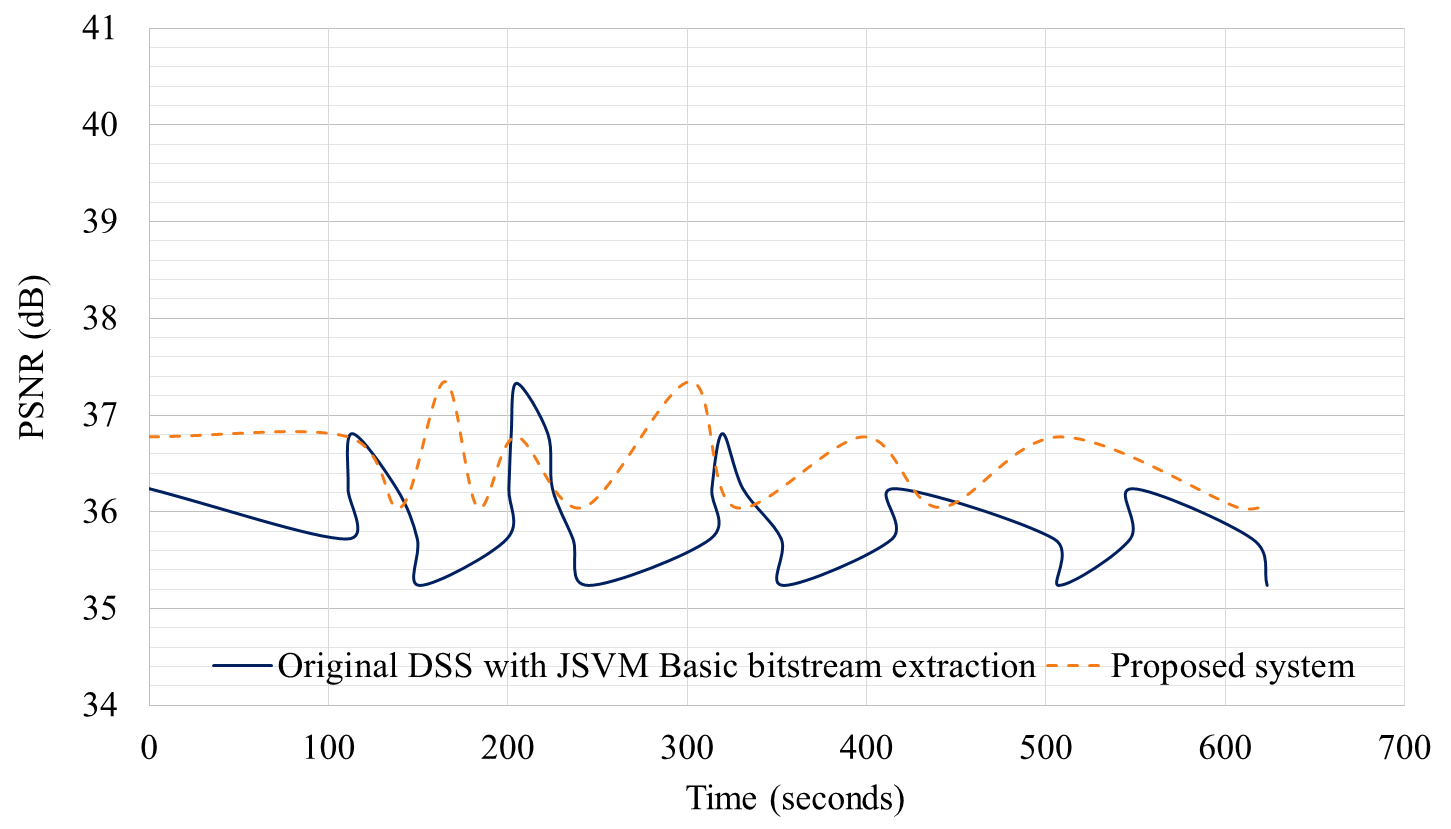
\includegraphics[width=0.47\textwidth]{figures/Fluctuation-PSNR1.png}
\label{fig:Fluctuation-PSNR1}}\hfill
\subfloat[带宽在600kbps附近波动:PSNR均值和方差在原始系统中是37.06和0.61,而在采用本文算法的系统中是37.32(提高了0.26)和0.33(降低了0.28)。]{
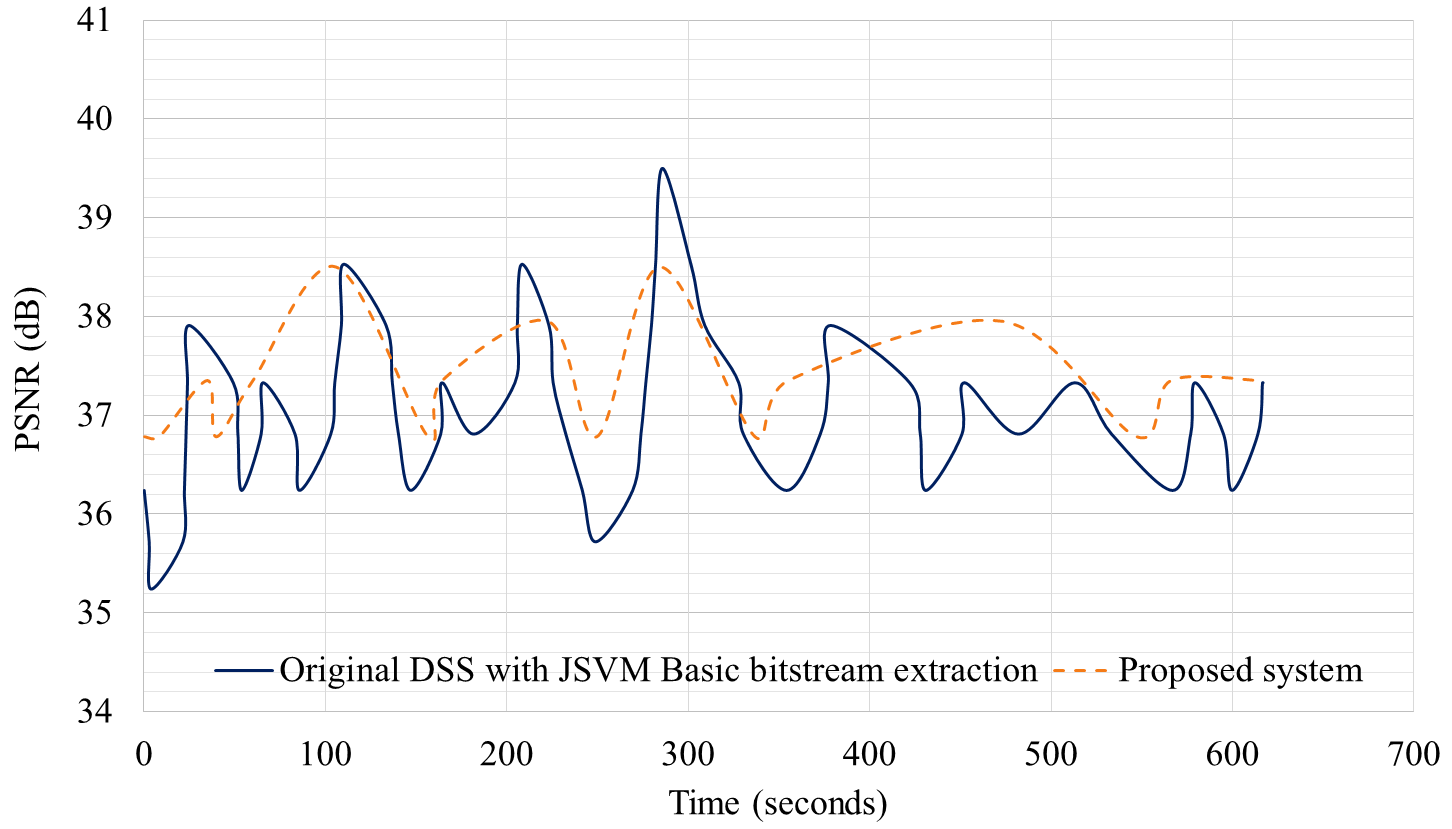
\includegraphics[width=0.47\textwidth]{figures/Fluctuation-PSNR2.png}
\label{fig:Fluctuation-PSNR2}}
\qquad
\subfloat[带宽在800kbps附近波动:PSNR均值和方差在原始系统中是37.92和1.24,而在采用本文算法的系统中是38.75(提高了0.83)和0.69(降低了0.55)。]{
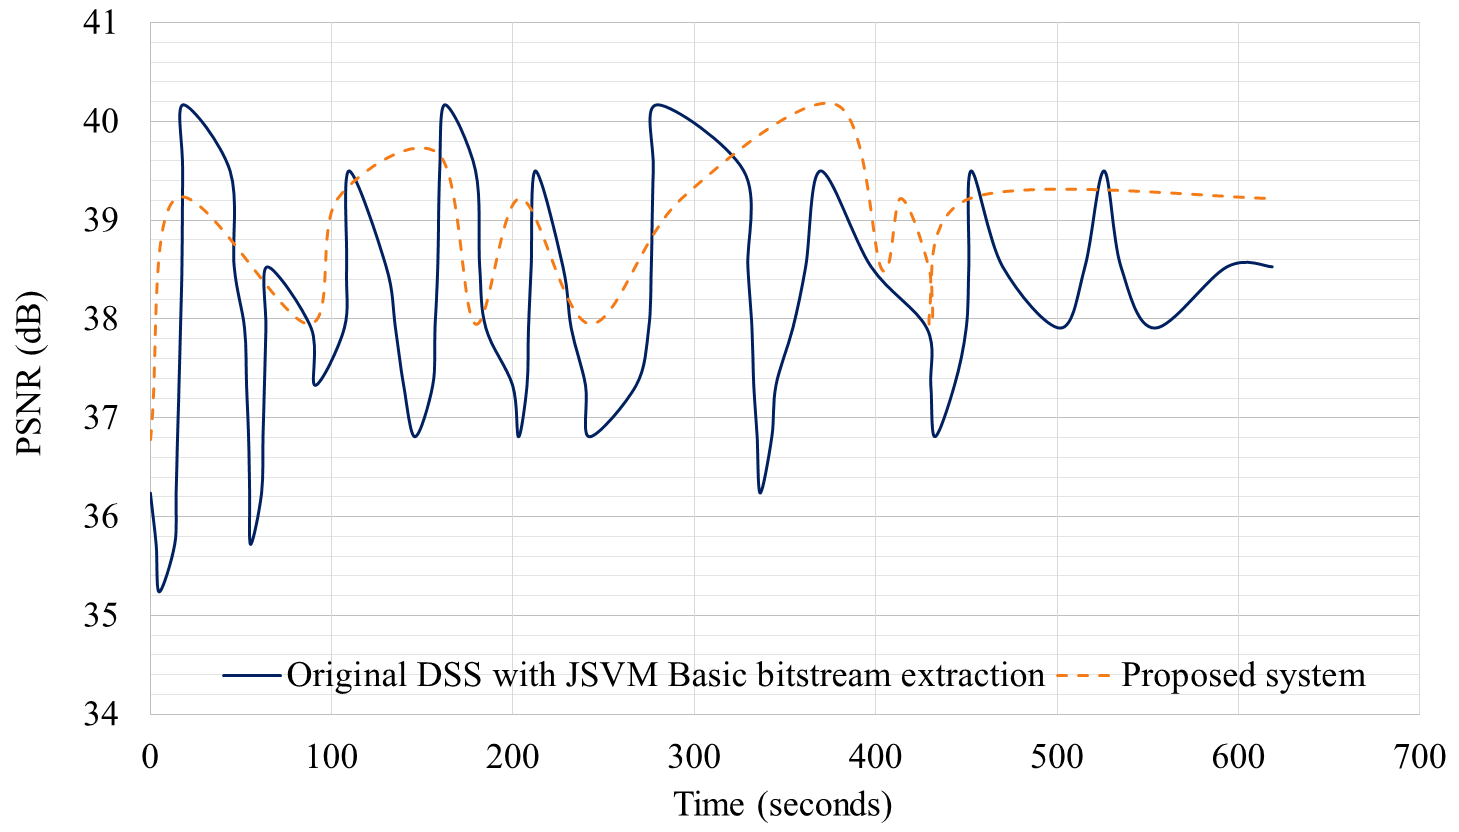
\includegraphics[width=0.47\textwidth]{figures/Fluctuation-PSNR3.png}
\label{fig:Fluctuation-PSNR3}}\hfill
\subfloat[带宽在1000kbps附近波动:PSNR均值和方差在原始系统中是38.28和1.30,而在采用本文算法的系统中是38.94(提高了0.66)和0.71(降低了0.59)。]{
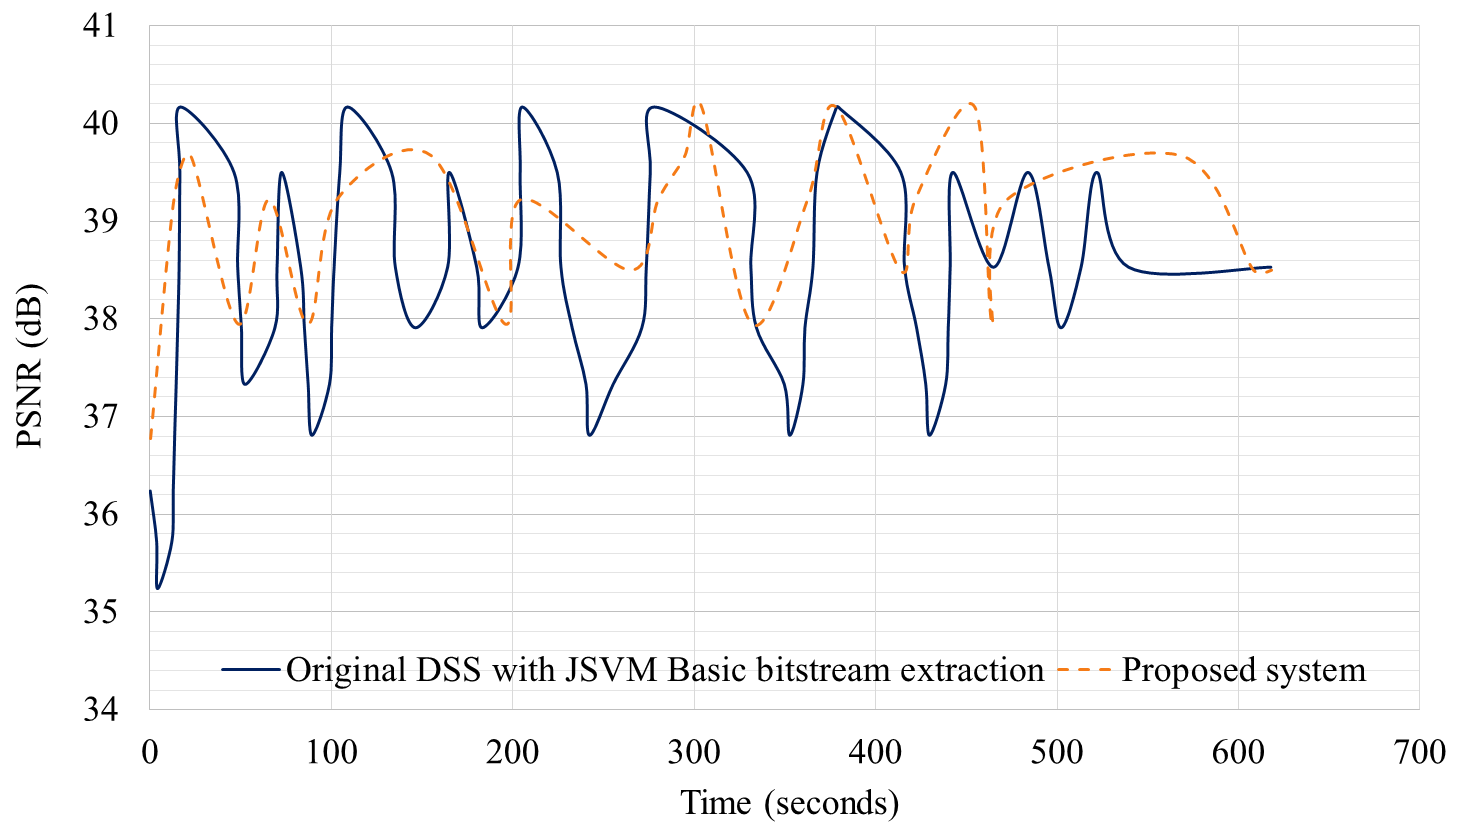
\includegraphics[width=0.47\textwidth]{figures/Fluctuation-PSNR4.png}
\label{fig:Fluctuation-PSNR4}}
\caption{不同流媒体系统所发送视频的PSNR随时间的变化情况
\label{fig:fluctuation-psnr}}
\end{figure*}


\subsection{用在直播系统中的效果}

为了对基于PID的直播系统内容发送码率自适应方法进行测试,我们实现了一个基于TCP的手机视频直播系统。我们选择业界已经广泛使用的RTMP协议作为应用层流媒体协议,具体实现采用了第三方开源的代码库librtmp\footnote{http://rtmpdump.mplayerhq.hu/librtmp.3.html}。我们用nginx-rtmp-module\footnote{https://github.com/arut/nginx-rtmp-module}帮助完成了中转服务器的搭建。我们采用了开源软件x264\footnote{http://www.videolan.org/developers/x264.html}作为视频编码器。我们在Android平台上实现了内容产生和上传的程序,集成了我们提出的自适应码率控制算法,并采用开源播放器ffplay\footnote{https://ffmpeg.org/}作为接收方,它可以播放RTMP协议的流媒体并对播放缓冲区长度进行预设。我们通过动态改变内容产生方所连接的路由器所允许的最大带宽来模拟出波动的网络状况。

在我们的实验中,采集帧率设置为15 FPS,过程变量$\overline{S_{ASB}(t)}$的控制目标值$\tau$设为15(单位是数据段的个数,每个数据段含有一个GOP的视频),改变码率的单位为20kbps,初始码率为500kbps,对系统状态的检查周期为2秒。我们调节得到的PID控制参数$K_p$、$K_i$和$K_d$分别为0.8,0.13以及0.07。我们在3种条件下进行测试:(1)固定带宽为1Mbps;
(2)长周期波动带宽,带宽每隔40秒变化一次,在200kbps到1.4Mbps之间波动;(3)短周期波动带宽,在200kbps到1.4Mbps之间随机波动。测试结果参见图\ref{fig:09}。

\begin{figure}
	\centering
	\subfloat[1Mbps的固定带宽的实验结果]{\label{fig:09-1}\includegraphics[width=0.8\textwidth]{clip/09-1.png}} \\
	\subfloat[长周期波动带宽的实验结果]{\label{fig:09-2}\includegraphics[width=0.8\textwidth]{clip/09-2.png}} \\
	\subfloat[短周期波动带宽的实验结果]{\label{fig:09-3}\includegraphics[width=0.8\textwidth]{clip/09-3.png}}
	\caption{直播系统在不同测试条件下码率随时间变化的情况}
	\label{fig:09}
\end{figure}

从图\ref{fig:09-1}中可以看出,我们提出的方法使得码率在35秒以内保持上升,直到趋近带宽。从图\ref{fig:09-2}和\ref{fig:09-3}可以看出,通过我们的方法进行的调整,在一个合理的延迟以内,码率和波动的带宽基本保持同步,而且对带宽的频繁变化做了一定的平滑。总之,加入PID码率自适应算法比不进行码率调整的直播效果有所改善。


\section{本章小结}

本章首先对PID控制器的基本思想做了简单介绍,然后将其用到了视频流媒体中的码率自适应问题中。在选择了合适的过程变量与控制目标之后,对通用PID模型稍作修改,得到了更加直观有效的基于比例的模型,并据此给出了码率自适应算法(又称为质量控制算法)。所提出的算法相比于其他算法不仅提高了所发送视频的平均质量,还降低了质量波动,取得了更好的平滑性。当流媒体服务器把最佳视频码流传送给用户后,在下一章中我们讨论如何对视频流的解码过程进行优化,以确保尽可能多的客户端设备能达到播放高清甚至超高清视频的条件。
	\chapter{基于缓冲区分析的直播码率自适应算法}

很多现有的实时流媒体系统都是建立在UDP协议之上,相比于TCP协议而言,在带宽较低以及丢包率较高的网络中,UDP是一个更好的选择。在这样的网络状况下,TCP协议的实用性很弱,因为它的重传机制以及拥塞控制导致低吞吐量,带来难以接受的传输延迟。而UDP带来的实时性效果显著强于TCP,因为传输的数据包大小更小,并且不确保数据的完整接受。

然而,正因为UDP的不可靠的端对端传输,我们需要在更高层的协议之上进行大量特殊的处理,实现对传输过程进行控制以及对传输数据进行校验。而在另一方面,网络状况已经得到了持续快速的改善,使用TCP传输流媒体数据的可行性大大提高。因此,基于TCP的视频流媒体越来越成为关注的热点。渐进式HTTP视频流正广泛地应用在视频点播技术,并且通过HTTP Live Streaming(HLS)协议[1]扩展到视频直播领域。Real Time Streaming Protocol(RTSP)[2]以及Real Time Streaming Protocol(RTMP)[3]是两种业界广泛应用的,能够实现低延迟传输以及连接端进行消息交互的流媒体协议。这些基于TCP的技术很容易使用,并且在稳定的网络状况下具有良好的效果。然而,对于不稳定的移动网络,TCP吞吐量的变化仍然需要有效的应对,从而实现更好的流媒体用户体验。

在大多数的相关研究在两个层面处理TCP吞吐量的变化:传输层以及应用层。在传输层中,主要有两类方案。一类是通过修改TCP协议的重传机制和拥塞控制机制来降低吞吐量的波动[4][5],另一类是TCP传输层的信息建模来实现准确估计吞吐量从而选择最佳的视频编码参数。然而这一些方法难以具体实现,并且不能被应用在现有的基于TCP的应用层协议中。在应用层方面,研究主要集中在Dynamic Adaptive Streaming over HTTP(DASH)[6],它提供了客户端动态切换码率的机制来实现连续而平滑的视频点播服务。基于DASH的方案也同样被应用在HLS中实现自适应的直播视频流。然而DASH的自适应机制针对接收端,而不是内容提供方,因此不能应用在用户生成内容(UGC)的直播系统中。

在这篇论文中,我们提出一种通用的针对应用层的自适应码率控制方法来适应TCP吞吐量的变化,我们使用多缓冲模型来分析传输过程,并采用缓冲区的状态来评估网络状况。通过在这个模型获取到的信息,我们提出一种基于PID的自适应码率控制算法,能够灵敏地调节视频码率来匹配当前的网络吞吐量,从而在保证流畅播放的情况下提供最高能达到的视频质量。我们还对调节过程进行优化,使其尽可能稳定和准确。我们基于RTMP协议实现了手机视频直播系统,并采用了这种方法。我们在变化的网络状况下,实现了相对流畅的视频播放,并取得了高带宽利用率。
这篇论文剩下的部分主要包含以下内容:第二部分是传输架构的概述,第三部分描述了多缓冲模型,第四部分详细介绍了基于PID的自适应码率控制算法,第五部分展示了在不同条件下的实验结果,第六部分进行了总结。

\section{视频直播系统概述}

在有些视频直播系统中,视频内容由服务器或者与服务器通过局域网连接的设备生成。在这种情形下,视频直播和视频点播具有很多共同点。在直播中服务器将动态生成的视频数据发送给客户端,和点播最主要的区别在于传输速率不能超过视频数据生成速率,因此当所有生成的数据都传输之后,客户端需要等待下一个数据片段就绪\supercite{Thang2014}。而在如今十分火热的用户生成内容(UGC)直播模式下,服务器本身不充当初始的内容产生方,在其他设备上持续生成的视频内容经过不确定且不可忽略的延迟传输到中转服务器。目前已经非常普及的智能手机成为了理想的内容产生方和接收方。图\ref{fig:07}展示了通用的手机视频直播系统的主要模块。集成了高效视频编码器的智能手机,将实时视频数据传输到接收服务器,在此同时,原始视频流被转码成多路具有不同码率的视频流。客户端可以通过当前网络环境选择最合适的码率,从服务器获取视频数据。

\begin{figure}[h]
	\centering
	\includegraphics[width = 0.9\linewidth]{clip/07.png}
	\caption{通用的手机直播系统模型\label{fig:07}}
\end{figure}

为了提供高质量的直播视频流,内容产生方需要传输尽可能高码率的视频,这可能导致每个数据段传输时间过长,造成接收端的播放中断。而内容产生方在变化的网络状况下尽可能利用网络吞吐量传输高质量视频的同时保证接收端的流畅播放,是一个挑战。与此同时,延迟需要控制在一个可以接收的范围。我们在内容产生方设计了一个上传码率自适应控制器,这种方案能够应用于UGC的视频直播。

简单起见,我们假设服务器具有快速的内部操作,同时接收端通过稳定高效地网络与服务器进行连接,这意味着服务器和接收端的视频流与内容产生方和服务器的视频流保持同步。这个假设对我们的研究重点没有影响。我们将传输架构简化成如图\ref{fig:08}所示。内容产生方的编码器将输入视频压缩之后传递给基于TCP的应用层协议。经过各层协议的封装,数据被传递到网络进行实际传输。在接收端经过一个逆向过程之后,数据输入到解码器进行解码,然后在播放器中进行渲染。与此同时,在发送方的自适应控制器每隔特定的周期对传输信息进行检查,并采用后文将介绍的特定的策略对编码器参数进行调整。

\begin{figure}[h]
	\centering
	\includegraphics[width = 0.9\linewidth]{clip/08.png}
	\caption{简化的直播系统传输架构\label{fig:08}}
\end{figure}

\section{直播中的多缓冲区模型}

\subsection{TCP缓冲区}

几乎所有的现代操作系统都集成了TCP协议,它是一种网络传输层协议。在传输过程当中,TCP协议采用了一种滑动窗口机制来保证可靠性,同时控制流量。为了实现滑动窗口机制,采用了TCP发送缓冲区(TSB)来缓存将要发送的数据同时维护滑动窗口,以及TCP接收缓冲区(TRB)来缓存接收成功但未被上层协议获取的数据。TSB中的数据收在到接收确认之后才会被移除,而TRB中的数据在被上层协议获取之后才会被移除。只有当TRB中存在足够空间的时候,网络传输才会进行。

\subsection{应用层发送缓冲区}

根据TCP的传输过程,只有当TSB中存在足够空间的时候,上层协议才能够将数据放入TSB。否则,上层协议的进程将会被阻塞,等待TSB中缓存的数据被移除。我们将第$i$次阻塞时间表示为$\varDelta t(i)$,将传输视频的帧率表示成$f$,并假设每一个数据段内的视频帧数为$n$。如果对于所有的$i$,都满足$\varDelta t(i) \le n/f$,那么这是较为理想的情况,因为不存在发送数据的积累。否则,在产生阻塞的时候需要采用应用层发送缓冲区(ASB)来缓存持续产生的视频数据。当TSB中产生足够的空间的时候,ASB队列头部的数据将会被移除进行发送。我们定义ASB的长度为其中数据段的数量,在大多数情况下我们期望它是一个较小的值。在通常情况下,存在ASB的最大长度。如果ASB达到了最大长度,后面到来的数据段将会被丢失。ASB长度上限的设置是一种通用的限制延迟的方法。

\subsection{播放缓冲区}

当ASB的长度增长的时候,发送端将在大于$n/f$的间隔时间收到两个连续的数据段。在这种情况下,为了保持连续的播放,几乎所有播放器都会设置一个播放缓冲区(PB),它从TRB中获取数据,并按照固定的速率将数据解码并显示。当PB的长度的为0时,视频停止播放直到PB的长度增长到一个固定值。我们称这个值为初始值,并表示为$S_0$。在很多系统中,这种方法被证明十分有效,它弥补了短时间视频码率和网络带宽的不匹配,有效减少了视频中断的现象。通常情况下,$S_0$就是PB的最大长度,达到$S_0$的时候数据段在接收端将被丢弃。

图\ref{fig:20}展示了接收端的数据曲线。$G(t)$表示在时间$t$之前在内容产生方生成的数据段的数量,因此$G(t) = \mu t$,其中$\mu$是一个常量,表示数据段生成的速率。$A(t)$和$P(t)$表示在接收端接收到和播放的数据段的数量,图中有$S(t) = A(t) - P(t)$。第一个数据段在经过传输延迟$d_t$之后到达接收端,PB开始接收到数据。我们假设在时间$t_0$,第一次使得$S(t_0)=S_0$,开始进行播放。$t_0$可以看做播放延迟,我们表示成$d_p$。因此,存在$S(t) \le \mu (d_p - d_t)$。当$S(t)$减小到$0$,播放终止,直到$S(t)$重新增长到$S_0$。

\begin{figure}[t]
	\centering
	\includegraphics[width = 0.8\linewidth]{clip/20.png}
	\caption{直播系统接收端数据关系\label{fig:20}}
\end{figure}

\subsection{多缓冲区模型分析}

如上文所讨论的,在传输架构中有四个缓冲区:TCP发送缓冲区、TCP接收缓冲区、应用层发送缓冲区、播放缓冲区,他们组成了多缓冲系统。在图\ref{fig:21}中,$G(t)$、$P(t)$以及$A(t)$与上一小节讨论的定义相同,$D(t)$表示在时间$t$之前进入TSB的数据段数量。我们使用$S_b(t)$表示在时间$t$存在于缓冲区$b$的数据段的数量。因此存在:
\begin{equation}
\label{eq:mm-1}
S_{ASB}(t)=G(t)-D(t),
\end{equation}

\begin{equation}
\label{eq:mm-2}
S_{TSB}(t)=D(t)-A(t),
\end{equation}

\begin{equation}
\label{eq:mm-3}
S_{TRB}(t)=A(t)-A(t)=0,
\end{equation}

\begin{equation}
\label{eq:mm-4}
S_{PB}(t) =A(t)-P(t),
\end{equation}

\begin{equation}
\label{eq:mm-5}
S_{ASB}(t)+S_{TSB}(t)+S_{TRB}(t)+S_{PB}(t)=G(t)-P(t).
\end{equation}


公式\ref{eq:mm-3}表示TRB的大小为0,因为在TRB中所有完整的数据段都会迅速被获取。当,即播放进行的时候,存在$G(t)-P(t)=\phi$,$\phi$是一个常量,反映了播放延迟。因此我们可以得到
\begin{equation}
\label{eq:mm-6}
S_{ASB}(t)+S_{PB}(t)=\phi-S_{TSB}(t).
\end{equation}
当$S_{ASB}(t)=0$,$S_{TSB}(t)$被$A(t)$所决定,它反映了网络状况。当$S_{ASB}(t)>0$时,意味着在发送数据到TSB时发生了阻塞,TSB一直处于充满状态,$S_{TSB}(t)$达到了上限,我们表示为$\alpha$。在这种情况下,存在
\begin{equation}
\label{eq:mm-7}
S_{ASB}(t)+S_{PB}(t)=\phi-\alpha=\delta.
\end{equation}
这表示着可以通过ASB的变化来控制和估计PB的变化。当$0 < S_{PB}(t) \le S_0$的时候,播放是连续的,可以通过保持$\delta - S_0 \le S_{ASB}(t) < \delta$进行实现,其中$\delta \ge S_0$。为了实现最小的延迟,$\delta$期望被设置为$S_0$。

\begin{figure}[t]
	\centering
	\includegraphics[width = 0.8\linewidth]{clip/21.png}
	\caption{多缓冲区模型结构图\label{fig:21}}
\end{figure}

多缓冲系统的信息在应用层可以被很容易地获取,我们可以根据这些信息在内容产生方设计一个自适应控制器来执行自适应码率控制。


\section{码率自适应算法}

在这一部分,我们详细介绍自适应码率控制方法。我们希望自适应过程实现以下几个目标:(1)接收端能够连续播放;(2)传输和当前吞吐量匹配的最高视频质量;(3)尽可能低的延迟;(4)在快速波动的网络状况下灵敏地自适应;(5)方法具有通用性,能够容易地实现。对于目标(5),我们的方法建立在通用的基于TCP的模型上,并采用了应用层参数。对于目标(3)和(4),我们考虑了最小可调度单元(MSDU)。对于目标(1)和(2),我们提出了一种新的基于PID控制的方法,能够动态地将系统保持在理想状态。

\subsection{最小可调节单元}

我们定义MSDU为我们能够完整传输或丢弃的最小的单元。在我们所讨论的系统中,MSDU为数据段。数据段的小大可以在两个方面对系统产生影响:(1)传输延迟,数据段中的数据越多,第一个数据段完整到达接收端需要的时间就越长;(2)自适应的灵敏度,一次自适应调整只有在正在进行的传输过程结束之后才会起作用。因此我们期望数据段的大小能够最小。

在基于DASH的方案中,为了实现高度灵敏的切换,图像组(GOP)被设定为数据段[12]。一个GOP可以单独播放,包含了一个I帧以及多个P帧。当一个GOP被丢弃时,对其他的GOP没有影响。通常一个GOP的持续时间是1到5秒。

在我们的方法中,我们将MSDU设置为视频帧,这样可以讲传输延迟最小化,以及将自适应的灵敏度最大化。当一帧被丢弃时,我们需要丢弃其整个GOP中后续的P帧,这样不会带来解码的错误。

\subsection{状态变量选取}

使用PID进行码率自适应的关键在于选取一个能够反映传输状况的过程变量。基于TCP的直播系统在传输过程中有四个缓冲区,分别是应用层发送缓冲区(ASB)、TCP发送缓冲区(TSB)、TCP接收缓冲区(TRB)、播放缓冲区(PB)。这几个缓冲区的关系和意义如图\ref{fig:20}和\ref{fig:21}所示。其中对内容产生方最重要的信息是ASB内的数据长度,记为$S_{ASB}(t)$(在时刻$t$的值),它能够直接反映视频码率和吞吐量之间的匹配情况。当视频码率高于当前的吞吐量时,该缓冲区内的数据长度趋向于增大,否则保持相对稳定或者减小为0。理想状况下,它首先应该是一个大于0的值,以保证接收方播放不中断;其次它不应该太大,否则意味着发送码率太高。所以,我们选择$S_{ASB}(t)$作为系统的过程变量,而选择一个接近0的常量$\varepsilon$作为控制目标。

然而,如果网络吞吐量在一个小的范围频繁波动,将使得系统变量值不稳定而且相对随机,导致不必要的频繁的调整。为了消除这样的随机性,我们将过程变量的定义修改为$\overline{S_{ASB}(t)}$,它表示在时刻$t$之前的一个时间段$\tau$内$S_{ASB}(t)$的平均值。它可以表示为:
\begin{equation}
\label{eq:asb}
\overline{S_{ASB}(t)} = \dfrac{1}{\tau} \int_0^\tau {S_{ASB}(t)}\: .
\end{equation}

对于UGC直播应用来讲,由于发送的码流是实时生成的,所以调整码率时直接改变编码器参数以改变生成码率即可,不需要涉及码流截取等数据源端的操作。但是,质量等级的概念仍然需要,它在这里变成了改变码率的单位。控制模型可以直接采用原始PID中的做法,用过程变量和$\varepsilon$的差值来计算比例、积分、微分这几个部分。具体的算法流程以及三个PID参数的选取和调优与上一小节中的相同,这里不再详述。

\subsection{算法描述}

\section{实验结果}

\subsection{实验配置}

为了对基于PID的直播系统内容发送码率自适应方法进行测试,我们实现了一个基于TCP的手机视频直播系统。我们选择业界已经广泛使用的RTMP协议作为应用层流媒体协议,具体实现采用了第三方开源的代码库librtmp\footnote{http://rtmpdump.mplayerhq.hu/librtmp.3.html}。我们用nginx-rtmp-module\footnote{https://github.com/arut/nginx-rtmp-module}帮助完成了中转服务器的搭建。我们采用了开源软件x264\footnote{http://www.videolan.org/developers/x264.html}作为视频编码器。我们在Android平台上实现了内容产生和上传的程序,集成了我们提出的自适应码率控制算法,并采用开源播放器ffplay\footnote{https://ffmpeg.org/}作为接收方,它可以播放RTMP协议的流媒体并对播放缓冲区长度进行预设。我们通过动态改变内容产生方所连接的路由器所允许的最大带宽来模拟出波动的网络状况。

\begin{figure}[!t]
	\centering
	\subfloat[1Mbps的固定带宽的实验结果]{\label{fig:09-1}\includegraphics[width=0.6\textwidth]{clip/09-1.png}} \\
	\subfloat[长周期波动带宽的实验结果]{\label{fig:09-2}\includegraphics[width=0.6\textwidth]{clip/09-2.png}} \\
	\subfloat[短周期波动带宽的实验结果]{\label{fig:09-3}\includegraphics[width=0.6\textwidth]{clip/09-3.png}}
	\caption{直播系统在不同测试条件下码率随时间变化的情况}
	\label{fig:09}
\end{figure}

在我们的实验中,采集帧率设置为15 FPS,过程变量$\overline{S_{ASB}(t)}$的控制目标值$\tau$设为15(单位是数据段的个数,每个数据段含有一个GOP的视频),改变码率的单位为20kbps,初始码率为500kbps,对系统状态的检查周期为2秒。我们调节得到的PID控制参数$K_p$、$K_i$和$K_d$分别为0.8,0.13以及0.07。我们在3种条件下进行测试:(1)固定带宽为1Mbps;
(2)长周期波动带宽,带宽每隔40秒变化一次,在200kbps到1.4Mbps之间波动;(3)短周期波动带宽,在200kbps到1.4Mbps之间随机波动。

\subsection{结果分析}

测试结果参见图\ref{fig:09}、\ref{fig:14}和表\ref{tab:live-bandwidth}、\ref{tab:live-playtime}。

\begin{figure}[!t]
	\centering
	\subfloat[1Mbps的固定带宽的实验结果]{\label{fig:14-1}\includegraphics[width=0.65\textwidth]{clip/14-1.png}} \\
	\subfloat[长周期波动带宽的实验结果]{\label{fig:14-2}\includegraphics[width=0.65\textwidth]{clip/14-2.png}} \\
	\subfloat[短周期波动带宽的实验结果]{\label{fig:14-3}\includegraphics[width=0.65\textwidth]{clip/14-3.png}}
	\caption{直播系统在不同测试条件下播放时间占比的变化情况}
	\label{fig:14}
\end{figure}

从图\ref{fig:09-1}中可以看出,我们提出的方法使得码率在35秒以内保持上升,直到趋近带宽。从图\ref{fig:09-2}和\ref{fig:09-3}可以看出,通过我们的方法进行的调整,在一个合理的延迟以内,码率和波动的带宽基本保持同步,而且对带宽的频繁变化做了一定的平滑。如表\ref{tab:live-bandwidth}所示,我们提出的算法对于条件(1)、(2)和(3)分别将带宽占用率提高到92.1\%、88.9\%以及87.1\%。

从图\ref{fig:14-1}可以看出,对于进行调整和未进行调整的视频流,播放基本都是连续的。从图\ref{fig:14-2}和\ref{fig:14-3}可以看出,未经过调整的视频流的播放过程被频繁地中断,而经过调整的视频流的播放过程在大部分时间是连续的。如表\ref{tab:live-playtime}所示,我们所提出的方法对于条件(2)和(3)分别将播放时间占比提高到97.3\%和96.1\%,因此显著提高了播放连续性。总之,加入PID码率自适应算法比不进行码率调整的直播效果有所改善。

\begin{table*}
	\centering
	\caption{直播系统实验中的带宽利用率}
	\label{tab:live-bandwidth}
	\begin{tabular}{c|*{2}{p{1.0cm}<{\centering}|}{p{1.0cm}<{\centering}}}
		\hline\hline
		& CB & LTBV & STBV \\ \hline
		自适应调整  & 92.1\% & 88.9\% & 87.1\% \\ \hline
		不进行调整 & 50.4\% & 64.7\% & 80.3\% \\ \hline
	\end{tabular}
\end{table*}

\begin{table*}
	\centering
	\caption{直播系统实验中的播放时间占比}
	\label{tab:live-playtime}
	\begin{tabular}{c|*{2}{p{1.0cm}<{\centering}|}{p{1.0cm}<{\centering}}}
		\hline\hline
		& CB & LTBV & STBV \\ \hline
		自适应调整  & 100\% & 97.3\% & 96.1\% \\ \hline
		不进行调整 & 100\% & 73.4\% & 71.5\% \\ \hline
	\end{tabular}
\end{table*}

\section{本章小结}

本章首先对PID控制器的基本思想做了简单介绍,然后将其用到了视频流媒体中的码率自适应问题中。在选择了合适的过程变量与控制目标之后,对通用PID模型稍作修改,得到了更加直观有效的基于比例的模型,并据此给出了码率自适应算法(又称为质量控制算法)。所提出的算法相比于其他算法不仅提高了所发送视频的平均质量,还降低了质量波动,取得了更好的平滑性。当流媒体服务器把最佳视频码流传送给用户后,在下一章中我们讨论如何对视频流的解码过程进行优化,以确保尽可能多的客户端设备能达到播放高清甚至超高清视频的条件。
	\chapter{总结和展望}
本章总结全文并展望未来工作。
	% 排版参考文献列表。
	\addcontentsline{toc}{chapter}{参考文献}
	{
	\wuhao
	\bibliographystyle{chinese}
	\bibliography{thesis}
	}
	% 以下为正文之后的部分,默认不进行章节编号。
	\backmatter
	% 致谢。
	\chapter{致谢}

感谢计算机所的老师、同学等所有在我读博士期间关心帮助过我的人。


	% 成果。
	\chapter{个人简历和在学期间研究成果}

\section*{个人简历}

1988年12月8日出生于河南省郑州市。

2007年9月考入清华大学自动化系,2011年7月本科毕业并获得工学学士学位。

2011年9月保送进入北京大学计算机科学技术研究所攻读博士学位至今。

\renewcommand{\labelenumi}{[\arabic{enumi}]}

\section*{发表或被接收的论文}
\begin{enumerate}
	\item \textbf{Shengbin Meng}, Jun Sun, Yizhou Duan, Zongming Guo, ``Adaptive Video Streaming with Optimized Bitstream Extraction and PID-based Quality Control'', IEEE Transactions on Multimedia (TMM), vol. 18, no. 6, pp. 1124-1137, June, 2016.
	\item \textbf{Shengbin Meng}, Jun Sun, Zongming Guo, ``Software Solution for HEVC Encoding and Decoding'', Proceedings of International Conference on Multimedia Modeling (MMM), Sydney, Australia, January 5-7, 2015.
	\item \textbf{Shengbin Meng}, Yizhou Duan, Jun Sun, Zongming Guo, ``Highly Optimized Implementation of HEVC Decoder for General Processors'', Proceedings of IEEE International Workshop on Multimedia Signal Processing (MMSP), Jakarta, Indonesia, September 22-24, 2014.
	\item \textbf{Shengbin Meng}, Jun Sun, Yilei Wang, Zongming Guo, ``A PID-based Quality Control Algorithm for SVC Video Streaming'', Proceedings of IEEE International Conference on Communications (ICC), Sydney, Australia, June 10-14, 2014.
	\item \textbf{Shengbin Meng}, Jun Sun, Yizhou Duan, Zongming Guo, ``An Efficient Method For No-Reference H.264/SVC Bitstream Extraction'', Proceedings of IEEE International Conference on Acoustics, Speech, and Signal Processing (ICASSP), Florence, Italy, May 4-9, 2014.
	\item Jiexi Wang, \textbf{Shengbin Meng}, Jun Sun, Zongming Guo, ``A General PID-based Rate Adaptation Approach for TCP-based Live Streaming Over Mobile Networks'', accepted by IEEE International Conference on Multimedia \& Expo (ICME), Seattle, USA, July 11-15, 2016.
\end{enumerate}

\section*{申请的专利}
\begin{enumerate}
	\item \textbf{孟胜彬},孙俊,段一舟,郭宗明;“视频质量控制方法和装置”;申请日期:2014\\年08月29日;申请号:201410428958.0。
	\item 王杰西,\textbf{孟胜彬},孙俊,郭宗明; “基于PID控制的视频直播传输控制方法及系统”;申请日期:2016年03月03日;申请号:201610121496.7。
	\item 林镇安,\textbf{孟胜彬},孙俊,郭宗明;“流媒体音频同步方法及装置”;申请日期:2016年01月18日;申请号:201610031208.9。
	\item 刘森,\textbf{孟胜彬},孙俊,郭宗明;“视频质量控制方法”;申请日期:2015年05月08日;申请号:201510231060.9。
	\item 王杰西,\textbf{孟胜彬},孙俊,郭宗明; “基于WebRTC的交互式直播方法及装置”;申请日期:2015年05月07日;申请号:201510230757.4。
\end{enumerate}

\section*{参与的课题项目}
\begin{enumerate}
	\item 国家自然科学基金面上项目“高效可伸缩视频的编码、分析和调度研究”,项目号:61271020。
	\item 863项目“真三维视频紧凑表示与高效压缩”,项目号:2015AA011605。
\end{enumerate}
	% 原创声明和使用授权说明。
	{
	\CTEXsetup[
		format+ = {\centering}, beforeskip = {40bp}, afterskip = {15bp}
	]{section}

	\specialchap{北京大学学位论文原创性声明和使用授权说明}
	\mbox{}\vspace*{-3em}
	\section*{原创性声明}

	本人郑重声明:
	所呈交的学位论文,是本人在导师的指导下,独立进行研究工作所取得的成果。
	除文中已经注明引用的内容外,
	本论文不含任何其他个人或集体已经发表或撰写过的作品或成果。
	对本文的研究做出重要贡献的个人和集体,均已在文中以明确方式标明。
	本声明的法律结果由本人承担。
	\vskip 1em
	\rightline{%
		论文作者签名:\hspace{5em}%
		日期:\hspace{2em}年\hspace{2em}月\hspace{2em}日%
	}

	\section*{学位论文使用授权说明}

	本人完全了解北京大学关于收集、保存、使用学位论文的规定,即:
	\begin{itemize}
		\item 按照学校要求提交学位论文的印刷本和电子版本;
		\item 学校有权保存学位论文的印刷本和电子版,
			并提供目录检索与阅览服务,在校园网上提供服务;
		\item 学校可以采用影印、缩印、数字化或其它复制手段保存论文;
		\item 因某种特殊原因需要延迟发布学位论文电子版,
			授权学校在 $\Box$\nobreakspace{}一年 /
			$\Box$\nobreakspace{}两年 /
			$\Box$\nobreakspace{}三年以后在校园网上全文发布。
	\end{itemize}
	\centerline{(保密论文在解密后遵守此规定)}
	\vskip 1em
	\rightline{%
		论文作者签名:\hspace{5em}导师签名:\hspace{5em}%
		日期:\hspace{2em}年\hspace{2em}月\hspace{2em}日%
	}

	% 若需排版二维码,请将二维码图片重命名为“barcode”,
	% 转为合适的图片格式,并放在当前目录下,然后去掉下面 2 行的注释。
	%\vfill\noindent
	%\includegraphics[height = 5em]{barcode}
}


\end{document}

